%!TeX spellcheck = en-US

\documentclass[
    11pt, % The default document font size, options: 10pt, 11pt, 12pt
    %oneside, % Two side (alternating margins) for binding by default, uncomment to switch to one side
    english, % ngerman for German
    singlespacing, % Single line spacing, alternatives: onehalfspacing or doublespacing
    %draft, % Uncomment to enable draft mode (no pictures, no links, overfull hboxes indicated)
    %nolistspacing, % If the document is onehalfspacing or doublespacing, uncomment this to set spacing in lists to single
    %liststotoc, % Uncomment to add the list of figures/tables/etc to the table of contents
    %toctotoc, % Uncomment to add the main table of contents to the table of contents
    %parskip, % Uncomment to add space between paragraphs
    %nohyperref, % Uncomment to not load the hyperref package
    headsepline, % Uncomment to get a line under the header
    %chapterinoneline, % Uncomment to place the chapter title next to the number on one line
    %consistentlayout, % Uncomment to change the layout of the declaration, abstract and    acknowledgements pages to match the default layout
]{DoctoralThesis} % The class file specifying the document structure

\usepackage[utf8]{inputenc} % Required for inputting international characters
\usepackage[T1]{fontenc} % Output font encoding for international characters
\usepackage{mathpazo} % Use the Palatino font by default

% I AM NOT SURE I NEED THIS GEOMENTRY...
\geometry{
	paper=a4paper, % Change to letterpaper for US letter
	inner=2.5cm, % Inner margin
	outer=3.8cm, % Outer margin
	bindingoffset=.5cm, % Binding offset
	top=1.5cm, % Top margin
	bottom=1.5cm, % Bottom margin
	%showframe, % Uncomment to show how the type block is set on the page
}

\usepackage{natbib}
\usepackage{mathptmx}
\usepackage{amsmath}
\usepackage{amsfonts}
\usepackage{amssymb}
\usepackage[dvips,dvipdfm,pdftex]{graphicx}
\usepackage{pgfplotstable}
\usepackage{pgfplots}
\pgfplotsset{compat=newest}
\usepackage{array}
\usepackage{booktabs}
\usepackage{morefloats}
\usepackage{etex}
\usepackage{listings}
\usepackage{float}
\usepackage{epstopdf}
\usepackage[section]{placeins}
\usepackage[ruled,linesnumbered,resetcount,algochapter]{algorithm2e}

\newtheorem{definition}{Definition}

\usepackage[backend=bibtex,style=authoryear,natbib=true]{biblatex} % Use the bibtex backend with the authoryear citation style (which resembles APA)
\addbibresource{PhD_Thesis.bib} % The filename of the bibliography
\usepackage[autostyle=true]{csquotes} % Required to generate language-dependent quotes in the bibliography

%----------------------------------------------------------------------------------------
%	THESIS INFORMATION
%----------------------------------------------------------------------------------------

\thesistitle{Computational Open-Set Identification of The Web's ( Context ) Genres}
\supervisor{Dr. Efstathios \textsc{Stamatatos}}
% \examiner{} % Your examiner's name, this is not currently used anywhere in the template, print it elsewhere with \examname
\degree{Doctor of Philosophy} % Your degree name, this is used in the title page and abstract, print it elsewhere with \degreename
\author{Dimitrios A. \textsc{Pritsos}}
\addresses{} % Your address, this is not currently used anywhere in the template, print it elsewhere with \addressname
\subject{Computer Science} % Your subject area, this is not currently used anywhere in the template, print it elsewhere with \subjectname
\keywords{} % Keywords for your thesis, this is not currently used anywhere in the template, print it elsewhere with \keywordnames
\university{\href{http://www.aegean.gr}{University of Aegean}} % Your university's name and URL, this is used in the title page and abstract, print it elsewhere with \univname
% \department{\href{http://department.university.com}{Department or School Name}} % Your department's name and URL, this is used in the title page and abstract, print it elsewhere with \deptname
% \group{\href{http://researchgroup.university.com}{Research Group Name}} % Your research group's name and URL, this is used in the title page, print it elsewhere with \groupname
% \faculty{\href{http://faculty.university.com}{Faculty Name}} % Your faculty's name and URL, this is used in the title page and abstract, print it elsewhere with \facname

\AtBeginDocument{
\hypersetup{pdftitle=\ttitle} % Set the PDF's title to your title
\hypersetup{pdfauthor=\authorname} % Set the PDF's author to your name
\hypersetup{pdfkeywords=\keywordnames} % Set the PDF's keywords to your keywords
}

\begin{document}

\frontmatter % Use roman page numbering style (i, ii, iii, iv...) for the pre-content pages

\pagestyle{plain} % Default to the plain heading style until the thesis style is called for the body content

%----------------------------------------------------------------------------------------
%	TITLE PAGE
%----------------------------------------------------------------------------------------

\begin{titlepage}
\begin{center}

\vspace*{.06\textheight}
{\scshape\LARGE \univname\par}\vspace{1.5cm} % University name
\textsc{\Large Doctoral Thesis}\\[0.5cm] % Thesis type

\HRule \\[0.4cm] % Horizontal line
{\huge \bfseries \ttitle\par}\vspace{0.4cm} % Thesis title
\HRule \\[1.5cm] % Horizontal line

\begin{minipage}[t]{0.4\textwidth}
\begin{flushleft} \large
\emph{Author:}\\
\href{http://www.aegean.gr}{\authorname} % Author name - remove the \href bracket to remove the link
\end{flushleft}
\end{minipage}
\begin{minipage}[t]{0.4\textwidth}
\begin{flushright} \large
\emph{Supervisor:} \\
\href{http://www.aegean.gr}{\supname} % Supervisor name - remove the \href bracket to remove the link
\end{flushright}
\end{minipage}\\[3cm]

\vfill

\large \textit{A thesis submitted in fulfillment of the requirements\\ for the degree of \degreename}\\[0.3cm] % University requirement text
\textit{in the}\\[0.4cm]
\groupname\\\deptname\\[2cm] % Research group name and department name

\vfill

{\large \today}\\[4cm] % Date
%\includegraphics{Logo} % University/department logo - uncomment to place it

\vfill
\end{center}
\end{titlepage}


%----------------------------------------------------------------------------------------
%	ABSTRACT PAGE
%----------------------------------------------------------------------------------------
\begin{abstract}
\addchaptertocentry{\abstractname} % Add the abstract to the table of contents
The \textit{Web's Contexts Genres} computational identification is a subject where due to the advances of \textit{Machine Learning} research and technologies, created a fruitful environment for rejuvenating the interest of its research. The \textit{Identification of  the Genus} of the texts is a ascent task assigned to the Natural Language Processing and Information Retrieval research, since they have been digitized. In an attempt resolve the ambiguity of the Genus-taxonomy of the texts, it has been distinguished to the Genre, Register, Domain, ... taxonomies. In contrast to the others, Genre-taxonomy is more closely related to \textit{the style and the purpose} of the texts rather than their context. 

Since the explosion of the World Wide Web (a.k.a The Web) and the tremendous rate of context daily generation redefined and also is perpendicular to their Topic-taxonomy was the main issue. However, the scaling raised for more sophisticated approaches to handle the size of the information and increase the relevance of a potential query. \textit{Automated Web Genre Identification} can benefit all the advances of Computational Linguistics, Natural Language Processing and Information Retrieval by providing rich descriptions of the web documents, by narrowing the features, thus the vector, space for a Machine Learning algorithm to operate pattern recognition on texts and potentially help on building  more sophisticated data-structure such as the \textit{Ontology-Schemes}.

The contribution of this work on the field of Automated Web Genre Identification is mainly the establishment of a framework towards to its research as an open-set classification problem and the outcome to be valuable for realistic and practical applications. Particularly in this study the notion of the Noise is established, the proper evaluation methodology for AGI tasks has discovered. Most importantly two new machine learning algorithms has been build as an evolutionary step of their original versions. These algorithms are clearly showing that the feature selection and dimentionality reduction is closely tight to the model induction for the this task.

Finally, one will find the new avenues for improving the research on the field and understand the mechanics ruling the process of \textit{genre taxonomy evolution }and its \textit{characteristic temporal attribute}.  
\end{abstract}


%----------------------------------------------------------------------------------------
%	LIST OF CONTENTS/FIGURES/TABLES PAGES
%----------------------------------------------------------------------------------------
\tableofcontents % Prints the main table of contents
% \listoffigures % Prints the list of figures
% \listoftables % Prints the list of tables


\mainmatter % Begin numeric (1,2,3...) page numbering
\pagestyle{thesis} % Return the page headers back to the "thesis" styl

%----------------------------------------------------------------------------------------
%	THESIS INTRODUCTION
%----------------------------------------------------------------------------------------
\chapter*{Introduction}\label{sec:intro}

\addchaptertocentry{Introduction}
Computations \textit{Context Genre Identification} is the natural progress of the almost ancient process of categorizing the human intellectual creations on such an abstract taxonomy as their Genus. Artifacts such as paintings, music peaces and written texts are always a subject of research interest to be classified based on their from, style and communicative purpose other than their content. \textit{Literature or poems, impressionism or expressionism, blues or funky} are some examples of these artifacts genre which are independent of their topic.

This work is focused on the Text Genre-taxonomy and more specifically for the Web's Context Genres, motivated by its potential contribution towards the handling of the web content scale as the future concerns of the \textit{Information Retrieval (IR)} and \textit{Natural Language Processing (NLP)}. 

The ability to automatically recognize the genre of web documents can enhance modern IR systems by enabling genre-based grouping/filtering of search results or building intuitive hierarchies of web page collections combining topic and genre information \parencite{Braslavski2007,Rosso2008,de2009genre}. Similarly, the modern NLP systems for author attribution, automated translation can be benefit by narrowing the feature space for an algorithm model induction. The recognition of web genre can also enhance the effectiveness of processing the content of web pages in information extraction applications. For example, given that a set of web pages has to be part-of-speech tagged, appropriate models can be applied to each web page according to their genre \parencite{Nooralahzadeh2014}.

There also several research and application where the \textit{Automated Genre Identification (AGI)} advances can directly benefit them. Such as \textit{foreign language teaching} and \textit{journalism history research} where the genre-taxonomy is very important for locating the proper documents as a starting point for their work.

The \textit{Web Genre Identification  (WGI)} also can benefit a a search engine which it can provide its users with the option to define complex queries (e.g., blogs about machine learning or eshops about sports equipment) as well as the option to navigate through results based on genre labels (e.g. social media pages, web shops, discussion forum, blogs, etc).

However, research in WGI is relatively limited due to fundamental difficulties emanating from the genre notion itself. The most significant difficulties in the WGI domain are: (1) There is not a consensus on the exact definition of genre \parencite{crowston2011problems}; (2) There is not a common genre palette that comprises all available genres and sub-genres \parencite{santini2011cross,mehler2010genres_on_web,mason2009n,sharoff2010web}, moreover, genres are evolving in time since new genres are born or existing genres are modified \parencite{Boese2005}; (3) It is not clear whether a whole web page should belong to a genre or sections of the same web page can belong to different genres \parencite{jebari2015combination,madjarov2015web}; (4) Style of documents is affected by both genre-related choices and author-related choices \parencite{petrenz2011stable,Sharroff2010}. As a result, it is hard to accurately distinguish between personal style characteristics and genre properties when style is quantified.

Most previous studies in WGI consider the case where all web pages should belong to a predefined taxonomy of genres \parencite{Lim2005,santini2007automatic,kanaris2009learning,jebari2014pure_URL}. However, this naive assumption is not appropriate for most applications related with WGI. As in traditional text genres what are evolving in time, say novel to comics, forking and evolution, the same applies to Web-genres, say news to blog forking and to micro-blogging evolution. In fact the evolution of the web-genre taxonomy is even more rapid and the temporal idiosyncrasy of the genres more vivid. In addition to the scale of the Web where is intractable to locate all the possible genres in a given time, it is not possible to construct a universal genre palette. Thus there should always exist web pages that would not fall into any of the predefined genre labels.

In that sense the Web-pages \textit{Noise} is introduced and well defined in this study. {Noise} web-pages are considered also when multiple genres (predefined or not) co-exist \parencite{santini2011cross,levering2008using}. The vast majority of previous work in WGI avoid to examine the problems arising from the presence of noise and as a result it is not possible to estimate the effectiveness of most existing WGI approaches in realistic conditions.

The Genre-units are, also, discussed in this study such as \textit{the web-page, the web-page section, the web-page paragraph} or \textit{the web-site genres}. Consequently, the URL utility in the WGI task is raised and discussed in respect of the linking of these units and how it can be used as an indicator of the genre-identification. Then noise notion is changing slightly but the same approach can be applied to the one will be used when web-page is assumed as the main mono-genre unit.

To handle noise in WGI there are two options. First, to adopt the closed-set classification setup having one predefined category devoted to noise. Since this category would comprise all web pages not belonging to the known genre labels, it would not be homogeneous. Moreover, this noise class would be much more greater with respect to the other genres causing class imbalance problems. The second option is to adopt the open-set classification setting where it is possible for some web pages not to be classified into any of the predefined genre categories \parencite{pritsos2013open}. This setup avoids the problem of class imbalance caused by numerous noisy pages and also avoids the problem of handling a diverse and highly heterogeneous class. On the other hand, open-set classification requires strong generalization with respect to the closed-set setup \parencite{scheirer2013toward}.

Open-set classification framework is closely related to the Novelty Detection and the One-class Classification where it is assumed that only positive examples are available for the surprised model induction methods. These methods then have been adapted to this problem and there are several examples such as One-Class SVM, One-Class Neural Networks... etc. It might sound similar but it is not a binary classification setup for training these algorithms due to the lack of the negative examples. In respect of WGI this is the realistic case scenario where one might be able to collect a good sample (however not complete due to the scaling of the Web) for the positive samples but for the negative samples is virtually impossible since not even the temporal genre-taxonomy pallet is not available. 

As an even more complicated task the open-set classification usually (use Open set Classification Survey reference HERE) assumes a multi-class classification problem where a few genres might be available to the \textit{Learner} and again the total number of the negative samples are not available. Then several issues rise and the most important of all is to constraint the \textit{Open-Space Risk}. 

The {Open-Space Risk} is a definition for form the domain of Open-Set classification research to describe the weakness of the current closed-set ML algorithms usually are used out-of-the-box to regulate low Recall performance of the models due to the luck of negative samples. Usually also of the constraint positive samples. In order to measure the performance of such algorithms the \textit{Openness} test have very recently introduced. 

In this study is also confirmed and rediscovered the proper methods for measuring the performance of the open-set algorithms on the WGI task. Measure like $F_{1}$ statistic, \textit{Precision, Recall, Accuracy, Precision-Recall Curves (PRC) and PRC Area Under the Curve (AUC)} are inappropriate for the open-set classification where an algorithm can classify an arbitrary sample one one of it is \textit{Known} classes but it can also let the sample as \textit{Unknown} or in a "Don't know bucket". It is shown that the $Macro F_{1}$ form of the above measures it can tackle the problem of proper measurement and overcome the usually \textit{imbalanced available corpora} for the WGI research. 

In combination with the \textit{openness test} and the proper measurement it is presented in this work that simple \textit{Distance based algorithms} is a perspective approach towards the handling of the WGI task, comparing them to more sophisticated methods like SVM. It also the open-set Ensemble Learners are shown to have higher performance. 

In this study are introduced and tested two open-set classification models, the \textit{Random Feature Subspacing Ensembles} (RFSE) and the \textit{Open Nearest Neighbours Distance Ratio} OpenNNDR, as an evolutionary adaption for the WGI task, of two already suggested algorithms. 

The evaluation of these algorithms is mainly focuses on the textual information one can get from the web-pages such as Word n-grams (WNG), Character n-grams (CNG), Part-of-Speach n-grams (POSNG). However, there are several other features have been suggested in the related literature. All of them are presented in chapters \ref{} and an extra focus is given to some of the most notable ones other than the ones have been thoroughly tested in this study.

Starting with the \textit{Bag-of-word (BOW)} together with the Bag-of-HTML-tags ($BOT^{html}$) there was a great effort to exploit information one could get from the text and the html structure of the web-pages, where in the closed-set framework seemed to work. Several other approaches of the same pattern also have been tested such as the POS or the POSNG and eventually the best one could was from the CNG where after that more sophisticated features have been tried especially for more complex and more close to the real world scenario.

In other AGI cases where the Web was not in the main focus, also \textit{Superficial-Features} (SUF) where tested in combination usually to the BOW or more generally Bag-of-Terms (BOT) features. Such features where the \textit{length of words, paragraphs, stances Frequency's} or the \textit{Ration of the Max-to-Lengths} for the same patters of the text. Moreover, lexicographic, and morphological features are also testes.....

Most notably the Word-Graph connection was attempted to be exploited where the Graph properties measurement where used of  deriving good indicators for discriminating the genres. An even farther approach was to exploit the text structure of the URLs in the web-pages other than their Linking property discussed above....

All the above examples are heuristics and this was so far the main focus for the AGI/WGI research. Other heuristics where focusing on the amplification of the information by using not only the URL linking information but also the text of the neighbouring pages in order to enable an algorithm to classify, in a closed-set framework, an arbitrary web-page. 

There where not but a few attempts to approach the WGI in the open-set framework where the most notable is the case where and adaptive algorithm was presented with interesting results. However, its weakness to noise tolerance was found to be very high, which is something one would have been expected in the first place. 

In respect of the document representation usually the TF or the TF-IDF approach where used and most of the cases the results seems to be very closely related to the corpus the algorithms have been tested. However, there is one interesting case where a \textit{Ranking Vocabulary Distance} was used for the classification, where the representation and the decision method are tightly related.
 
Finally, this study have tested the Distributional Features (Word Embedding) modeling on the WGI task for the first time showing very interesting results. The \textit{Word Embedding} modeling method is using a multi-layer \textit{Neural Network (NNet} in order to project the word of the texts in a multi-dimensional feature space. The NNet modeling then is used in order to bring the word that are "similar" in the context of taxonomy-classes. In the end every word is encoded to this model with a fix-size vector. The same process can be followed an then a vector for each document....

Using two benchmark corpora we perform a systematic evaluation of WGI models when noise is either unstructured (the true genre of noisy pages is not available) or structured (the true genre of noisy pages is available). In order to handle the latter case, we employ the openness test in WGI that provides a detailed view of performance for a varying number of known/unknown labels. This test has already been used in visual object recognition \parencite{scheirer2013toward} and it perfectly fits the WGI task.

The rest of this work is organized as follows. In section ...


%----------------------------------------------------------------------------------------
%	THESIS CHAPTERS
%----------------------------------------------------------------------------------------
%!TeX spellcheck = en-US

\chapter{Web Genre Identification: A Survey}

\label{chap:relevant_work}

%----------------------------------------------------------------------------------------

% Define some commands to keep the formatting separated from the content
\newcommand{\keyword}[1]{\textbf{#1}}
\newcommand{\tabhead}[1]{\textbf{#1}}
\newcommand{\code}[1]{\texttt{#1}}
\newcommand{\file}[1]{\texttt{\bfseries#1}}
\newcommand{\option}[1]{\texttt{\itshape#1}}

%----------------------------------------------------------------------------------------

\section{Introduction}\label{chap:relevant_work:sec:intro}

The notion of \textit{Genre} in linguistics domain is an abstract taxonomy of the \textit{texts}, on which there is a great theoretical and mostly philosophical debate respectively to its internal mechanics of this taxonomy evolution. In computational linguistics domains is yet an other taxonomy where several computational methodologies has been developed for automating the process. All these methods are mainly based on \textit{Machine Learning (ML)} where most of the work historically has been focused on the raw text pre-processing and the feature selection methodologies. In addition, mostly out-of-the-box ML methods has been tested and some of its variations. Only recently there is a redirection of the research focus to the \textit{Vocabulary Learning Models (VLM)} which are used for feeding the input of the Identification or Classification ML models, instead of the \textit{Bag-of-Words (or Bag-of-Terms) BoT }\footnote{In this text Bag-of-Terms (BoT) is equivalent to the Bag-of-Words  (BOW), which has been widely used in the literature of the Information Retrieval and Natural Language Processing domains. Since, BoT is accurately describing the meaning of BOW in most of the cited literature.} model. This study is focude mostly on the Web-Genre Identification (WGI) computational methodologies, which is the main focus of the Natural Language processing and Information Retrieval research focus, in respect of the genre notion. Although there a several other text resources, other than the Web, where the Automated Genre Identification (AGI) has been also been studied and also are cited here.

Genre means "genus" in the Greek language and for the text focused studies (either traditional linguistics or computational) means style. The main utility of the genre taxonomy, or in other words the reason we like as humans to categorize and give a "genus" to our text is for speeding up the communication. Thus, what we mostly do with texts is to use a genre taxonomy for transferring or retrieving the information in the "speed" of a word (or word n-gram) when it comes to describe the texts.....

\textbf{NOTE: In this survey section the Genre and Web-Genre is studied mostly thematically than historically. However, wherever there is interesting historical sequence in the research field it is pointed out.}


Since 2013 the where two very informative research studies related to the utility, evolution, and recognition of the genre taxonomy. One (REF) from the discipline of the \textit{English for Academic Purposes} (EAP) where it was vividly discussed the divergence in the genre taxonomies between the difference academic disciplines and reasoned the utility of the genre taxonomy for enabling the teachers and the students to improve their rhetorical and written language with the purpose of improving the teaching procedure. What is important to note for this study is the conclusion that the same genre-type can be very different for the communication purpose, i.e. as text identity carrier, but it can also contain the same style and other language properties when the purpose is similar, for example the article of new paper and an article form a magazine where one can claim that they are a different genre-type although they governed by the same linguistic properties.

*** Genre variations in student .... (paper)
The types of their study genre taxonomy mainly focused on the \textit{purpose} of the students written context and less on the \textit{style}, thus their genre-types where \textit{Creative Writing, Response Paper, Critique/Evaluation, Argumentative Essay, Report, Research Paper and Proposal}. Their study was a manual statistical process, similar to a \textit{Data Mining} process where grammatical features were counted in the texts. Then these features where indicating the score for each of the four (4) dimensions which has been qualitatively predefined. The counting process was using a heuristic computational tagger, named as Biber tagger (see Biber 1988 or ???).   

On the other hand and other research lying in the discipline of cognitive computing an health research they found humans are recognizing the genre type of a document or web-page using other cognitive processes relates mostly to the formatting of the text. Particularly they used as well configured apparatus for tracking the eyes movement while the recognition effort, where they fount that the eyes where following specific paths and where stopping to special landmarks on the text. They have concluded that the process of genre recognition was mostly related to the format and not the context, in addition they statistically measured that they previews experience was not related to the recognition process. Although it was the previews knowledge of the text formatting was accelerating the process. However, on the opinion of the authors of this study the genre recognition is a more deep process, thus as one can concluded by reading their study the landmarks they are referring into seems to be the only context combined with the formatting of the text that the human brain is requiring for identifying the genre-type. Given that their study is focused on the e-mail genres where formatting options compare to the web or textbooks is rather limited is advocating the conclusion that the minimum context is required for identifying the genre-type.

They are discussing of tree main perception (psychology) theories, i.e. Gestaltism (or Gestalt psychology), Ecological and Constructivism, which are the theories which can interpret the perception procedures, it this case the eye movement on the texts, to the cognition process for identifying the genre types of the texts. The perception procedure includes some eye movements mainly doing two tasks, \textit{scanning} and \textit{skimming}. Theses two procedures are irrespective of the belief of the supported interpretation theory related to the internal thought process for making a genre taxonomy decision. Scanning is the process where more or less we are trying to locate information of interest where the information has a homogeneous property, such as the a phone number in phone-book list. Skimming is the process where we are trying to locate information of interest where the information is raw or without a specific form, such as names, verbs, or phrases that is related to the abstract related concept in order to decide whether the text is matches and worth farther reading. 

The process of scanning and especially skimming in practice follows some specific eye movements, i.e. Fixation and Saccadic. Saccadic is the process while scanning or skimming that the eye is jumping around to the text, while Fixation is the process where the eye remains focused for a while. One can resemble the process like navigation where the eye is constantly moving while is focused for small fragments of time in landmarks of interest.

\begin{figure}[t]
	\begin{center}
    	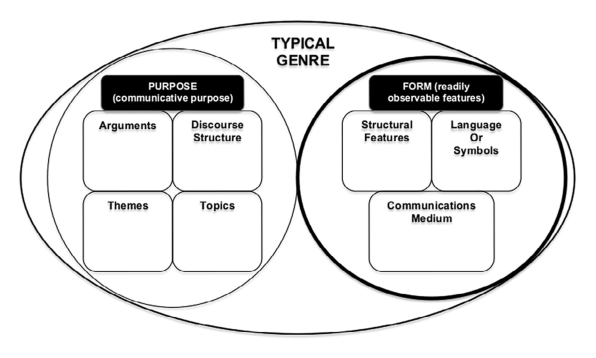
\includegraphics[scale=0.95]{Figures/Sotlen_diagram.eps}
		\caption{Stolen Imag.}
		\label{fiig:Stolen}
	\end{center}
\end{figure}

***
Genres, in textual sense, is sometimes defined as group of texts of documents that share a communicative purpose, as determined by the \textit{discourse community} which produces and/or reads them. "In \textbf{structurational}terms, genre are social institutions that are produced, reproduced, reproduced or modified when \textit{human agents} draw on genre rules to engage in organizational communication".

"Layout in organizational communities cause people to focus perceptually on key parts of the text and our \textbf{empirical research has previously demonstrated that people use layouts and other related cues to focus on key parts of the text.}"
***

A very recent research on Cross-Lingual Genre Classification showed that it is possible to get very good results when an ML model is trained with a corpus samples of one language and then testing the trained model to an other. However, the evaluation framework was closed-set and the relation of the languages seems to be of a great importance for the accuracy performance of the model. That is, in some cases it was important the language to be of the same group for example the Roman or the Slavic group of languages and for others was not. Some times oddly the performance was dropping when the language was form the same language group \parencite{nguyen2019cross}.

Web Genre Identification (WGI) concerns the association of web pages with labels that correspond to their form, communicative purpose and style rather than their content. The ability to automatically recognize the genre of web documents can enhance modern information retrieval systems by enabling genre-based grouping/filtering of search results or building intuitive hierarchies of web page collections combining topic and genre information \parencite{Braslavski2007,Rosso2008,de2009genre}. For example, a search engine can provide its users with the option to define complex queries (e.g., blogs about machine learning or eshops about sports equipment) as well as the option to navigate through results based on genre labels (e.g. social media pages, web shops, discussion forum, blogs, etc). The recognition of web genre can also enhance the effectiveness of processing the content of web pages in information extraction applications. For example, given that a set of web pages has to be part-of-speech tagged, appropriate models can be applied to each web page according to their genre \parencite{Nooralahzadeh2014}. However, research in WGI is relatively limited due to fundamental difficulties emanating from the genre notion itself.

\textbf{The most significant difficulties in the WGI domain are: (1) There is not a consensus on the exact definition of genre \parencite{crowston2011problems}; (2) There is not a common genre  palette that comprises all available genres and sub-genres \parencite{santini2011cross,mehler2010genres_on_web,mason2009n,sharoff2010web}, moreover, genres are evolving in time since new  genres are born or existing genres are modified \parencite{Boese2005}; (3) It is not clear whether a whole web page should belong to a genre or sections of the same web page can belong to  different genres \parencite{jebari2015combination,madjarov2015web}; (4) Style of documents is affected by both genre-related choices and author-related choices \parencite{petrenz2011stable,Sharroff2010}. As a result, it is hard to accurately distinguish between personal style characteristics and genre properties when style is quantified.}

As \textit{Web Search} from an extension of IR because the main subject under investigation \parencite{manning2008introduction}, \textit{Web page Genre Classification } is becoming the main subject of document classification research.

Most previous work in WGI follows a typical closed-set text categorization approach where, first, features are extracted from documents and, then, a classifier is built to distinguish between classes. Attention is paid to the appropriate definition of features that are able to capture genre characteristics and should not be affected by topic shifts or personal style choices. 

Blogs is a genre-type has attracted as special interest on its own, in differed domains such as in sociology, psychology, linguistics and mostly in computational linguistics and WGI. There are several blogs' properties of interest of the research and  also blogs having their own sub-genre taxonomy. Blog-taxonomy general genres are \textit{Filter, Personal-diary} and \textit{Notebook} and other related to the authors group of styles such as \textit{Reflective, Narrative, Emotional, Rational} and \textit{Personal , Non-Personal}. The thought research on the blog-types classification has delivered a set of special linguistic and web-page structural properties which are increasing the performance of the closed set classification. Details for this linguistic properties used for specially for blogs sub-taxonomy classification are described in section \ref{chap:relevant_work:sec:features:subsec:heuristics} \cite{virik2017blog,hoffmann2012cohesive,hoffmann2012cohesive,derczynski2014social,qu2006automated}. 

\section{Genre Definitions: The Linguistics and the Computational Linguistics}\label{chap:relevant_work:sec:linguistics_definition}

Overcoming the difficulties related to the genre taxonomy pointed out in linguistic and empirical studies, in text in \textit{text categorization} there is a great amount of work related to the automated categorization of texts based on \textit{genre taxonomy}. Although, starting from fundamentally different routes computational and linguistic studies, both ended up with the same notion of genre, which is eventually having two complimentary meanings,  i.e. \textit{Style} and \textit{Genus}\footnote{Genus in Greek means \textit{type} or \textit{class}} \parencite{sugiyanto2014term}. 

(DEFINITION DEBATE) In linguistic studies there is a great debate in defining \textit{the notion of genre} as an \textit{abstract categorization} of texts and the relation between them. Despite the methodological differences the linguistic community concluded that the idiosyncrasy of the \textit{genre taxonomy} is mutable and diverse \parencite{coutinho2009describe}. This kind of idiosyncrasy is yielded to the \textit{genre taxonomy} due to the spontaneous genesis of the genre classes. The genesis of a genre class is socio-centric interaction which is emerging from the need to describe the texts in order to accelerate the social communication procedure. Thus, genre classes are spontaneously emerging while the communication procedure is taking place.

(READERS PERCEPTION) Humans can efficiently recognize the genre-types by processing the texts intuitively. However, there is a \textit{great luck of consensus} for the genre-types, particularly naming the genres. There there was an effort of several user studies for eliciting the mechanics in the process of \textit{genre identification and tagging}. The results on user agreement were very discouraging. Also, when it come to the reporting, i.e. for humans to describe specifically the terms or/and the attributes with which they use to identify the genre-types then there is a great confusion. A convincing reasoning for that is the plethora of textual, stylistic and conceptual terms which are used where they are different per individual and/or per group (e.g. teachers, scientists, engineers) for the same (or similar) text (or web-page) \parencite{roussinov2001genre, crowston2011problems}. 

Researchers, of cognitive computing and health research disciplines, found humans are recognizing the genre type of a document (or web-page) using other cognitive processes related mostly to the form of the text. Particularly they used as well configured apparatus for tracking the eyes movement while the recognition effort. One can resemble the process like navigation where the eyes are constantly moving while they are focusing for small fragments of time in landmarks of interest. The pausing of the eyes on the text "landmarks" is called \textit{Fixation} while the "jumping" movements of the eyes is called \textit{Saccadic}. The whole process was the effort to locate information of interest such as a specific text forms, names, verbs, or phrases that are related to the abstract concept in order to decide whether the text is matches and worth farther reading. They systematically found that the process of finding the genre-type of the text is the same as to find out whether a text worth farther reading. Thus, the genre taxonomy definitely accelerates the communication procedure and helping the reader of the text find the information of interest faster \parencite{clark2014you}.

(WRITERS AWARENESS) In discipline of the \textit{English for Academic Purposes} (EAP)  it was vividly discussed the divergence in the genre taxonomies between the difference academic disciplines and reasoned the utility of the genre taxonomy for enabling the teachers and the students to improve their rhetorical and written language with the purpose of improving the teaching procedure. What is important to note for this study is the conclusion that the same genre-type can be vary differently form the communication purpose, i.e. as text identity carrier, but it can also contain the same style and other language properties when the purpose is similar, for example the article of new paper and an article form a magazine where one can claim that they are a different genre-type although they governed by the same linguistic properties. Therefore, for the witter of a text is is very important to be aware (thus to be taught) of the genre-type in order the text to be recognizable for the reader is seeking similar texts \parencite{hardy2016genre,melissourgou2017genre,al2017genre}.

(NEWS GENRE SUB-GENRES) The utility of the text genre identification (and/or classification) has been realized by the journalism historians. The technology advances and the new science innovations cased the attraction to the field. Journalism historians using a different genre-taxonomy where they mainly focusing on the purpose of the texts by analyzing the structure of the texts, where the structure consist of abstract elements. Their main genre-type are Inverted Pyramid, Martini Glass, Kabob, Narrative, Narrative and elements are \textit{Standard Lede, Body Section,  Narration, Synopsis, Image Lede}.  Similarly to the EAP domain, their sub-genre taxonomy is including genre-types like . \parencite{dai2018fine}.

(GENRE AS WRITING STYLE) The aforementioned variations of the genre taxonomy's notion is related more to the methodology and the objective of the text categorization task's specifications, rather than the philosophical difference. Particularly in author attribution domain there is a focus on identifying the \textit{style of the author} \parencite{stamatatos2009survey,koppel2011authorship,koppel2014determining}. On the other hand in the information retrieval (IR) domain, the interest is to classify the texts based on a predefined \textit{genre pallet}. Thus the interest is focused on the \textit{style of the authors group}, such as scientists, journalists, bloggers, etc.

(THE WEB GENRE) In consideration of \textit{the web genres taxonomy} it has been also eloquently analyzed the utilities and the difficulties for the web users. It has been pointed out that the genre taxonomy is summarizing the type and the style of the text in a single term as a communicative act [This conclusion cited also in \parencite{de2009genre}]. In the domain of \textit{web genre identification (WGI)}, \textit{the web genre taxonomy pallet} (which mostly used for research) has been formed in a top-down approach, where a group of experts are forming the taxonomy based on the specific objective of the task \parencite{crowston2011problems}. Moreover, in WGI research there was a very early observation that genre are organized in a hierarchical manner \parencite{wu2010fine}. Thus, most likely a web page might be multi-genre, the genre unit is considered to be the web-page \parencite{madjarov2015web,jebari2015combination}. However, in section \ref{???} there is a discussion related the web-genre units other than the web-page.

As described so far, after a significant amount of work related to the study of the \textit{Genre-Taxonomy} and the \textit{Genre-Identification}, there is an agreement for the criteria which are defining the genres and the  web-genres. That is, the \textit{Form} and the \textit{Function/Purpose}. Complimentary criterion is the \textit{Context}, for example, the genre-type of the \textit{academic home web-pages} are easily identified by their context. The computational process of a text's \textit{context} is a standard procedure for the \textit{Topic Identification}. Although text's topic is considered as orthogonal to its genre, in cases such as academic home web-pages some context indicators can be exploited for the identification, also, of the Genre \parencite{coutinho2009describe,crowston2011problems,kanaris2009learning,jebari2015combination,gollapalli2011identifying}. 

Considering the above, it is clear that the Web-Genre Taxonomy has also a relatively abstract notion where is slightly changes depending on the research framework, despite the fact that the criteria for the genre-types of the texts are more or less common. Thus, for continuing the a this study in for the computationally, particularly NLP, research approach we are defining the notion of web-genre-type as follows.   

\textbf{However, \textit{genre} itself requires different level of human reading abilities to be recognized and even with these skills different humans may disagree \parencite{mccarthy2009psychological}.}

\begin{definition} Web-Genre-Type is defined as a class where its samples are i.i.d. Thus every web-unit (usually web-page) is always derived under a unique class distribution and the class distributions are not overlapped. That is, the Genre-Taxonomy consist from a distinctive non-overlapping classes/types.
\end{definition}

\section{Machine-Learning Methodology for Web Genre Identification and Classification}\label{chap:relevant_work:sec:machine_learning_methods}

\textit{(SVM Based)} There are several studies where their perdition model was the infamous SVMin the closed set framework, either in multi-class or binary form \parencite{dai2018fine}. 

SVM, Naive Bayes, Random Forest, Decision Trees(C4.5), AdaBoost and several types of features.\parencite{lee2017text}. Where Random Forest and SVM were the top performing classification methods for the genre-classification task.

SVM closed-set classification was also used for cross-lingual closed-set classification \parencite{nguyen2019cross}. 

In \parencite{virik2017blog} SVM is compared with Naive Bayes Classifier and k-Nearest Neighbours on the classification accuracy for the Blogs' sub-genre taxonomy. Their preliminary analysis on the correlation of the linguistic features and the sub-genres of the blogs indicating that all three algorithms were expected to be successfully, however, SVM was a bit better in performance. 

It seems than SVM based algorithms are high performance learners for the genre and web-genre closed-set classification task either in the multi-class or in the binary form. However, in the case of the open-set classification the performance drops significantly as shown in several studies such as ..., where simpler ensembles based models seems to work with higher performance. 

Finally, we design news structure indicative features and train a Support Vector Machine (SVM) (Cortes and Vapnik, 1995) classifier to label each news article with one of the proposed news structures. Experimental results show that reasonable performance can be achieved for automatic structure-based news genre classification by using our structure indicative features, even though results on minority classes remain low.

Although, the traditional bag-of-words approach had better result with XABoost or other techniques been tested for over a decade on genre identification or/and particularly on WGI, distributional feature models are early showing their advantages over the TF-IDF (or TF alone) models[REF].

Additionally, other methods extending the ensembles methodology like Random Forests have been alo became popular[REF].

Concerning the classification models involved in WGI studies, when a given genre taxonomy is utilized and there is no noise, then well-known machine learning models, like SVMs, decision trees, neural networks, naive Bayes, Random Forests, etc. are used \parencite{Lim2005,santini2007automatic,kanaris2009learning,jebari2015combination,sharoff2010web}. In case of presence of  noise, in a clustering framework described in \parencite{kennedy2005automatic} one cluster is built for each predefined class and another cluster is built for the noise. However, the most  common approach to handle noise is to build binary classifiers where the positive class is based on a certain predefined category and the negative class is based on the concatenation of  all other predefined categories plus the noise \parencite{kennedy2005automatic,dong2006binary,levering2008using}. Such a combination of binary classifiers can also be seen as a multi-label  and open-set classification model where a web page can belong to different genres and it is possible for one page not to belong to any of the predefined genres. More concrete open-set  classification models for WGI were presented in \parencite{stubbe2007genre,pritsos2013open}. However, these models were only tested in noise-free corpora \parencite{pritsos2015clef}. More  recently, Asheghi \parencite{Asheghi2015} showed that it is much more challenging to perform WGI in the noisy web in comparison to noise-free corpora.

To begin with, Kanaris and Stamatatos \parencite{kanaris2009learning} recently proposed a method for extracting an \textit{variable length n-gram corpus dictionary} for training an SVM model with a sample points projected in a feature space defined by this dictionary. The dictionary composed from a mixture of 3-grams, 4-grams and 5-grams, carefully selected from a modified version of \textit{LocalMaxs }algorithm. The algorithm was using a \textit{``glue function''} for selecting the most informative n-grams and the rest of them where discarded. Their \textit{``glue''} function was based on the frequency of n-grams in the corpus and not to any other feature selection method such as \textit{information gain}, in order to be portable to other corpora for farther evaluation.  

(Distance Based)
(Neural Based)
Recently Neural Networks have been used for modeling the WGI task (and other text classification tasks), additionally or independently of the Vocabulary modeling where neural-models have widely used. 

Most notably is the used of Recurrent Neural Networks (RNN) where Lingusistc Complegoty Countours (LCC) where employeed as modeling features (LCC details are explained in section \ref{chap:relevant_work:sec:intro:subsec:heuristics}). Their model was based on 32 LLC features where feeded to 32 Gated Recurrent Units (GRU)  and the output of each GRU was also fed to the next. Then all the output GRU output was the input of a Dense Layer of the RNN where a Softmax decision function was applied on. Their model was a closed-set framework with very high performace where was reaching over $90\%$  accuracy. (\parencite{strobel2018text}

(Clustering Based)
(Open Set Classification)

\section{Web Genre Noise and the Open-set approach}\label{chap:relevant_work:sec:intro}
Most previous studies in WGI consider the case where all web pages should belong to a predefined taxonomy of genres \cite{Lim2005,santini2007automatic,kanaris2009learning,jebari2014pure_URL}. Putting this setup under the vantage point of machine learning, it is the same as assuming what is known as a closed-set problem definition. However, this naïve assumption is not appropriate for most applications related to WGI as it is not possible to construct a universal genre palette a priori nor force web pages to always fall into any of the predefined genre labels. Such web pages are considered \textit{noise} and include web documents where multiple genres co-exist~\cite{santini2011cross,levering2008using}. 

Santini~\cite{santini2011cross} defines \textit{structured noise} as the collection of web pages belonging to several genres, unknown during training. Such structured noise can be used as a negative class for training a binary classifier \cite{Vidulin2007}. However, it is highly unlikely that such a collection represents the real distribution of pages of the web at large. On the other hand, \textit{unstructured noise} is a random collection of pages \cite{santini2011cross} for which no genre labels are available. The effect of noise in WGI was first studied in \cite{shepherd2004cybergenre,kennedy2005automatic,dong2006binary,levering2008using}.

Open-set classification models for WGI were first
described in~\cite{pritsos2013open,stubbe2007genre}. However, these models were only tested in noise-free corpora \cite{pritsos2015clef}. Asheghi~\cite{Asheghi2015} showed that it is much more challenging to perform WGI
in the noisy web setup in comparison to noise-free corpora. Recently, \textit{Ensemble Methods} were shown to achieve high effectiveness in open-set WGI setups~\cite{pritsos2018open}.
φ

To handle noise in WGI there are two options. First, to adopt the closed-set classification setup having one predefined category devoted to noise. Since this category would comprise all web pages not belonging to the known genre labels, it would not be homogeneous. Moreover, this noise class would be much more greater with respect to the other genres causing class imbalance problems. The second option is to adopt the open-set classification setting where it is possible for some web pages not to be classified into any of the predefined genre categories \parencite{pritsos2013open}. This setup avoids the problem of class imbalance caused by numerous noisy pages and also avoids the problem of handling a diverse and highly heterogeneous class. On the other hand, open-set classification requires strong generalization with respect to the closed-set setup \parencite{scheirer2013toward}.

Santini \parencite{santini2011cross} defines \textit{structured noise} as the collection of web pages belonging to  several genres. Such structured noise can be used as a negative class for training a binary classifier \parencite{Vidulin2007}. However, it is highly unlikely that such a collection  represents the real distribution of pages on the web. On the other hand, \textit{unstructured noise} is a random collection of pages \parencite{santini2011cross}. The effect of noise in WGI  was first studied in \parencite{shepherd2004cybergenre,kennedy2005automatic} where predefined genres were personal, organizational, and corporate home pages while noise consisted of non-home  pages. However, the distribution of pages into these four categories was practically balanced, hence it was not realistic. Dong et al.\parencite{dong2006binary} uses noise as the majority  class in an experiment where 190 instances from personal homepage, FAQ, and e-shop categories were used in combination with 600 noise pages. Similarly, Levering et al \parencite{levering2008using} uses about 200 instances for the predefined genres of store homepages, product lists, and product descriptions in combination with about 800 other pages (noise).

The majority of previous studies in WGI disregard the presence of noise. Santini \parencite{santini2011cross} defines \textit{structured noise} as the collection of web pages belonging to several genres. Such structured noise can be used as a negative class for training a binary classifier \parencite{Vidulin2007}. However, it is highly unlikely that such a collection represents the real distribution of pages on the web. On the other hand, \textit{unstructured noise} is a random collection of pages \parencite{santini2011cross}. The effect of noise in WGI was first studied in \parencite{shepherd2004cybergenre,kennedy2005automatic} where predefined genres were personal, organizational, and corporate home pages while noise consisted of non-home pages. However, the distribution of pages into these four categories was practically balanced, hence it was not realistic. Dong et al.\parencite{dong2006binary} uses noise as the majority class in an experiment where 190 instances from personal homepage, FAQ, and e-shop categories were used in combination with 600 noise pages. Similarly, Levering et al \parencite{levering2008using} uses about 200 instances for the predefined genres of store homepages, product lists, and product descriptions in combination with about 800 other pages (noise).

Concerning the classification models involved in WGI studies, when a given genre taxonomy is utilized and there is no noise, then well-known machine learning models, like SVMs, decision trees, neural networks, naive Bayes, Random Forests, etc. are used \parencite{Lim2005,santini2007automatic,kanaris2009learning,jebari2015combination,sharoff2010web}. In case of presence of noise, in a clustering framework described in \parencite{kennedy2005automatic} one cluster is built for each predefined class and another cluster is built for the noise. However, the most common approach to handle noise is to build binary classifiers where the positive class is based on a certain predefined category and the negative class is based on the concatenation of all other predefined categories plus the noise \parencite{kennedy2005automatic,dong2006binary,levering2008using}. Such a combination of binary classifiers can also be seen as a multi-label and open-set classification model where a web page can belong to different genres and it is possible for one page not to belong to any of the predefined genres. More concrete open-set classification models for WGI were presented in \parencite{stubbe2007genre,pritsos2013open}. However, these models were only tested in noise-free corpora \parencite{pritsos2015clef}. More recently, Asheghi \parencite{Asheghi2015} showed that it is much more challenging to perform WGI in the noisy web in comparison to noise-free corpora.

One of the most recent approaches related to the open-set classification on the \textit{Text Classification} problem was suggesting the reduction of the \textit{open space risk} using an SVM based methodology. Particularly, they are comparing 8 SVM based methods (additionally with an EM Semi-supervised method) in a open-set setup compare to their SVM Center-Based Similarity Space Learning SVM methods also in a open-set setup. Their method outperformed the other methods significantly with some exceptions. 

Their main contribution is the transitions of the problem form the \textit{feature space} to the \textit{distance space}. Particularly they are using ten (10) different centroids one for each of the five (5) different distance measures proposed by (Fei and Liu 2015......) and for two (2) different document representations one for uni-grams and one for bi-grams. Their centroids are calculated using  eq \ref{eq:manning_centroids} 

\begin{equation}\label{eq:manning_centroids}
	c_{j} = \frac{\alpha}{\lvert D_{+} \rvert} \sum_{d_{i} \in D_{+}} \frac{x_{j}^{i}}{\lVert x_{j}^{i} \rVert } - \frac{\beta}{\lvert D - D_{+} \rvert} \sum_{d_{j} \in D - D_{+}} \frac{x_{i}^{j}}{\lVert x_{i}^{j} \rVert}
\end{equation}

where $D_{+}$ is the set of documents in the positive class and $\lvert . \rvert$ is the size of function. $\alpha$ and $\beta$ are parameters, which are usually set empirically.

The SVM methods under testing where 1-vs-rest multi-class SVM (Platt200...), 1-vs-set Machine SVM \cite{scheirer2013toward}, W-SVM (Scheirer2014....), $P_{1}$-SVM (Jain2014), $P_{1}$-SVM (Jain2014), Exploratory Seeded K-means (Exploratory EM) (Dalvi2013...). They have also used a kind of \textit{openness testing}, by using $25\%$ to $100\%$ of the classes and their method were mostly outperforming the other methods. The macro-F1 score range of their methods from the most open set-up to the totally closed (i.e. using the $100\%$ of the classes) was from $0.417$ to $0.873$ depending on the corpus and the special class set-up \parencite{fei2016breaking}.

\section{Features (???and Dimensions???) extraction or selection}\label{chap:relevant_work:sec:features}

 To this end, several document representation features have been proposed and are related with textual content, e.g. character n-grams, word n-grams, part-of-speech histograms etc. \parencite{kumari2014web,petrenz2011stable,mason2009n,sharoff2010web} as well as the form, structure, and visual appearance of web documents, e.g., html tags, number of images, scripts etc. \parencite{Lim2005,levering2008using}. Usually, the combination of features from different sources enhances the robustness of WGI approaches \parencite{levering2008using,kanaris2009learning}.

Great attention historically on WGI has been given to the appropriate definition of features that are capable of capturing genre characteristics --- which includes but are not limited to character n-grams or word n-grams, part-of-speech histograms, the frequency of the most discriminative words, etc.  \cite{kanaris2009learning,kumari2014web,levering2008using,Lim2005,mason2009n,onan2018ensemble,petrenz2011stable,sharoff2010web}. Additionally, some additional useful features might come from exploiting HTML structure and/or the hyperlink functionality of web pages \cite{abramson2012_URL,asheghi2014semi,jebari2014pure_URL,priyatam2013don_URL,zhu2011enhance}. Recently deep learning methods have also been tested in genre detection setups with promising results~\cite{worsham2018genre}. 

A great variety of features to quantify the stylistic choices related to genre have been proposed in previous work. These are mainly based on textual content (e.g., character and word  n-grams) \parencite{mason2009distance,Sharroff2010} and form or structure of the web page (html tags, image count, links count, etc.) \parencite{Lim2005,levering2008using}. Both sources of  information are useful and usually their combination enhances a WGI model \parencite{kanaris2009learning}. However, features extracted from textual content are more robust since they do not  depend on technology or format used to create a web page and therefore they are more likely to remain stable in time.

 Several text  representation schemes based on textual content are examined and we focus on the appropriate selection of parameter settings for each model. Using two benchmark corpora we perform a  systematic evaluation of WGI models when noise is either unstructured (the true genre of noisy pages is not available) or structured (the true genre of noisy pages is available). In order  to handle the latter case, we employ the openness test in WGI that provides a detailed view of performance for a varying number of known/unknown labels. This test has already been used in  visual object recognition \parencite{scheirer2013toward} and it perfectly fits the WGI task.

 For example, given that a set of web pages has to be part-of-speech tagged, appropriate models can be applied to each web page according to their genre \parencite{Nooralahzadeh2014}

There are several other approaches on the problem of WPGC such as the use of part-of-speech and other linguistic facents as \textit{terms types} \parencite{feldman2009classifying,santini2005linguistic}, or even studies on the use of pure structural information of a web page,i.e. the HTML tags, instead of the text of these pages {[}Philipp Scholl{]}. However, in all studies in WPGC there are some important issues related to the experimental framework used from most of these studies that so far haven not been tackles. The most important of them is the size of the corpora which is extremely small to the size of the web (obviously) but is not even a good representative sample of the genres they include. This issues raised from Santini and Serge \parencite{santini2009web} on their paper that pointing out the issues of the current corpora and a road map of what should be done. 


***************************************
This part should be added to the Open-set Classfication chapter

\section{Re-defining the open space Risk }

The open space risk in \cite{scheirer2013toward} is originally defined as in eq. \ref{eq:the_original_open_space_risk}

\begin{equation}\label{eq:the_origina_open_space_risk}
	R_{o}(f) = \frac{\int_{o} f_{y}(x) dx}{\int{S_{o}}  f_{y}(x) dx}
\end{equation}
where $R_{o}(.)$ is the open-space risk function and $f_{y}(x)  \in \{0, 1\}$ is the classification function of class $y$, where $1$ is for recognizing its class and $0$ when not. $S_{o}$ is the large hyper-sphere where all the positive training data points and the \textit{positive open space area} $O$. 
The original formulation of the eq. \ref{eq:the_original_open_space_risk} $O$ area cannot be constrained by any means. The only information we are getting is the farther form the training date we go the risk of miss-classification is increasing One method to constrain the problem is by using the center of the positively labeled training data and defining a radios $r_{o}$ where it will reduce the open space area based on the positively labeled empirically observations. Then the $O$ is defined by the equation eq. \ref{eq:openspace_spherical_constrained}

\begin{equation}\label{eq:openspace_spherical_constrained}
	O = S_{o} - B_{r_{y}}(C_{y})
\end{equation}
where $B_{r_{y}}(.)$ is the function which defines the area of radius $r_{y}$ of the $C_{y}$ class defined by its training data \parencite{fei2016breaking}.

*******************************

\subsection{Heuristics has been used with success in WGI}\label{chap:relevant_work:sec:features:subsec:heuristics}
Focusing mainly in methodologies where the Prepossessing Heuristics has been used with great success in WGI.

There are several study approaches either in computational linguistics or in linguistics statistical approaches, where several heuristics has been proved to be efficient in extracting informative indicators for recognizing ans discriminating the genres. Usually it is required a more complex or sophisticated combination of text characteristics and not just word, character on n-gram (of both characters or words) counting. Such characteristics can be grammatical, syntactical, formatting and their combinations with  with counting or superficial information such the cases explained in ref{} paragraph.

Starting with \textit{Writing Style Features} and \textit{Key Event Placement (KEP) Features} improving significantly the performance of an out-of-the-box SVM classifier \parencite{dai2018fine}.  The writing style features were features extracted as a combination of also complex features, i.e. the combination of \textit{grammar production rules (GPR} and features from a semantic category of a \textit{Linguistic Inquiry and Word count (LIWC)} dictionary. GPR was also the combination of POS and word lexical rules and LIWC was a sophisticated dictionary of occurrences of word from a word category. The KEP was a set of text formatting

features or one could say "landmarks"such as characters, time, location in specific areas of the text. In practice it was the \textit{words overlapping count} between the first paragraph and the the title of the text The combination of both these structured based complex features where improved the macro-F1 performance from $47.9\%$ to $51.60\%$. In addition the micro-F1 was reaching $71\%$. 

Another notable methodology in respect of  feature selection and document representation is the \textit{Complexity Measures (CM)}.  Particularly a sliding window of characters and words is considered over a text. Then using this window several heuristics and superficial metrics are counted and/or calculated. Particularly them there are 32 of them as depicted in table \ref{chap:relevant_work:tbl:complexity_measures}. These features can be categorized in the following four (4) classes: (1) \textit{Raw Text Features} such as the Mean Sentence Length, (2) \textit{Lexical Features} such as Type Token Ration, (3) \textit{Morpho-Syntactic Features} such as Lexical Density of say verbs, (4) \textit{Syntactic Features},such as \textit{Complex Nominals} per Term Unit \parencite{strobel2018text}.

\begin{table}[t]
	\center
	\caption {Complexity Measures table as found in \parencite{strobel2018text}.}\label{chap:relevant_work:tbl:complexity_measures}
	\begin{tabular}{lll}
		\hline
		CM Name & Definition & NLP Category \\
		\hline
		Number of Different Words / Sample & $Nw_{diff} / Nw$ & Lexical \\
		Correct Type-Token Ration & $T/\sqrt{2N}$ & Lexical \\
		Number of Different Words & $Nw_{diff}$ & Lexical \\
		Root Type-Token Ration & $T/\sqrt{N}$ & Lexical \\
		Type-Token Ration & $T/N$ & Lexical \\
		Lexical Density & $N_{lex}/N$ & Morpho-Syntactic \\
		Mean Length Clause & $N_{W}/N_{C}$ & Morpho-Syntactic \\
		Mean Length Term-Unit & $N_{W}/N_{T}$ & Morpho-Syntactic \\
		Sequence Academic Formula List & $N_{seq}/AWL$ & Raw text \\
		Lexical Sophistication (ANC) & $N_{ANC}/N_{Lex}$ & Raw text \\
		Lexical Sophistication (BNC) & $N_{BNC}/N_{Lex}$ & Raw text \\
		Kolmogorov Deflate & KS2011 & Raw text \\
		Morphological Kolmogorov Deflate & KS2011 & Raw text \\
		Syntactic Kolmogorov Deflate & KS2011 & Raw text \\
		Mean Length Sentence & $N_{W}/N_{S}$ & Raw text \\
		Mean Length of Words & $N_{C}/N_{W}$ & Raw text \\
		Words on New Academic Word List & ${N_{W^{AWL}}}$ & Raw text \\
		Words not on General Service List & $\neg{N_{W^{GSL}}}$ & Raw text \\
		Clause per Sentence & $N_{C}/N_{T}$ & Syntactic \\
		Clause per Term-Unit & $N_{C}/N_{T}$ & Syntactic \\
		Complex Nominals per Clause & $N_{CN}/C$ & Syntactic \\
		Complex Nominals per Term Unit & $N_{CN}/N_{T}$ & Syntactic \\
		Complex Terms Units per Term Unit & $N_{CT}/N_{T}$ & Syntactic \\
		Coordinate Phrase per Clause & $N_{CP}/N_{C}$ & Syntactic \\
		Coordinate Phrase per Clause & $N_{CP}/N_{T}$ & Syntactic \\
		Dependent Clause per Clause & $N_{DC}/N_{C}$ & Syntactic \\
		Dependent Clause per Terms Unit & $N_{DC}/N_{T}$ & Syntactic \\
		Mean Length of Words (syllables) & $N_{Syl}/N_{W}$ & Syntactic \\
		Noun Phrase Post-modification (words) & $N_{NP^{Post}}$ & Syntactic \\
		Noun Phrase Pre-modification (words) & $N_{NP^{Pre}}$ & Syntactic \\
		Noun Phrase Pre-modification (words) & $N_{NP^{Pre}}$ & Syntactic \\
		Term Units per Sentence & $N_{T}/N_{S}$ & Syntactic \\
		Verb Phrase per Term Unit &  $N_{VP}/N_{T}$ & Syntactic \\
		\hline
	\end{tabular}
\end{table}

 An other very interesting set of features are the superficial, such as \textit{colon frequency, document length, sentence mean length and single-sentence paragraph count}. These features were successfully used as in input to an SVM classifier for a closed-set cross-lingual genre classification task. Particularly as mentioned in section \ref{chap:relevant_work:sec:intro} superficial information related only to the formatting of the text was successfully used for genre classification where training and testing were applied on different languages\parencite{nguyen2019cross}.
 
Blogs is a genre with special interest for the research communities and there are several studies analyzing aspects of sentiment classification and sub-genre or topic (or combination of all) taxonomy classification and/or identification. Such an analysis requires special feature extraction such as from\textit{ Lexical Analysis, Morphological Analysis, Lightweight Syntactical Analysis} and \textit{Structural Analysis}. In table \ref{chap:relevant_work:tbl:blogs_special_features} all the linguistic properties used for blogs sub-genre classification are presented in detail. In \parencite{virik2017blog} there is a detailed analysis for the correlation of the linguistic features and the blog-genres such as; \textit{informative, affecting, reflective, narrative, emotional} and \textit{rational}.

\begin{table}[t]
	\center
	\caption {Blogs' special features table as found in \parencite{virik2017blog}.}\label{chap:relevant_work:tbl:blogs_special_features}
	\begin{tabular}{p{4cm}p{7cm}p{3cm}}
		\hline
		Type & Description & NLP Category \\
		\hline
		Special Character Frequency & Frequency of: @, \#, \$, \%, <WhiteSpace>,\&, -, =, +, !,  ¿, ¡, [, ], /, | & Lexical \\
		Word Count & Number of alphanumeric tokens & Lexical \\
        Unique Lemma Count & Number of unique identified tokens & Lexical \\
        Abbreviation Frequency & Ration of abbreviations to all words & Lexical \\
        Ratio of long to short words & Long words consist of three and more syllables & Lexical \\
        Misspelled words Frequency & Ration of misspelled words of all words & Lexical\\
		Noun Frequency & Ration of nouns to all words & Morphological \\
        Adjective Frequency & Ration of adjectives to all words & Morphological \\
        Pronoun Frequency & Ration of pronouns to all words & Morphological \\
        Verb Frequency & Ration of verbs to all words & Morphological \\
        Proper Noun Frequency & Ration of proper nouns to all words & Morphological \\
        Ratio of Open to Closed words Classes & Words open to Inflection which include nouns, adjectives, pronouns, numerals, and verbs  & Morphological \\
        Ratio of functional to Content words Classes & Words with only grammatical function. Content words include nouns, adjectives, numerical, non-modal verbs and adverbs  & Morphological \\
        Frequency of sequences of functional words & Five of more consecutive functional words with tolerance of one closed word & Morphological \\
		Sentence Count & Number of identified sentences & Syntactical \\
        Average Sentence Count & Average sentence length in number of words & Syntactical \\
        Ratio of Simple to Compound Sentences & Compound consist of two or more sentences & Syntactical \\
        Average Sub-sentence Count & Sub-sentence is simple sentence inside a compound sentence & Syntactical \\
        Dominant Tense of  Predicted Candidates & Present, future and past & Syntactical \\
        Dominant Person of  Predicted Candidates & First, second and third & Syntactical \\
        Dominant Number of  Predicted Candidates & Singular and plural & Syntactical \\
		Link Frequency & Ration of number of Links to number of Sections  & Structural \\
        Image Frequency & Ration of number of Images to number of Sections  & Structural \\
        Section Count & Number of Sections & Structural \\
        Standard Deviation of Section length & Deviation of the number of words in sections & Structural \\
		\hline
	\end{tabular}
\end{table}


An other set of features used for genre classification of video content based on its text subtitles and descriptions is depicted in table \ref{chap:relevant_work:tbl:videogenre_textbased_special_features}. In this study the text, mainly the subtitles, was nte only source for classifying the videos, e.g. movies or TV-series. The have used a combination of BOW, superficial and syntactical features. Superficial features in this study were called \textit{content-free} and the ones related to specific words called \textit{content-specific} \parencite{lee2017text}. In the process they found that not all these features where so important where the most important of them were token-type ration, words per minute, characters per minute, Hapax legomena, Dis legomena, Short words ratio, Rations of  (10, 4, 3, 1)-letter words. 

\begin{table}[t]
	\center
	\caption {Video content genre classification special features, based exclusively on text (subtitles etc) table as found in  \parencite{lee2017text}.}\label{chap:relevant_work:tbl:videogenre_textbased_special_features}
	\begin{tabular}{p{4cm}p{7cm}p{3cm}}
		\hline
		Type & Description & NLP Category \\
		\hline
		Average words per minute & & Textual/Superficial  \\
        Average characters per minute & & Textual/Superficial  \\
        Average word length & & Textual/Superficial  \\
        Average sentence length in terms of words & & Textual/Superficial  \\
        Type/token ratio & Ratio of different words to the total number of words & Textual/Superficial  \\
        Hapax legomena ratio & Ration of once-occurring words to the total number of words  & Textual/Superficial  \\
        Dis Legomena ratio & Ration of twice-occuring words to the total number of words  & Textual/Superficial  \\
        Short words ratio & Words less than 4 characters to the total number of words & Textual/Superficial  \\
        Long words ratio & Words more than 6 characters to the total number of words & Textual/Superficial  \\
        Words-length distribution & Ratio of words in length of 1-20 & Textual/Superficial  \\
        Function words ratio & Ratio of function words to the total number of words  & Textual/Superficial  \\
        Descriptive words to nominal words ratio & Adjectives and adverbs to the total number of nouns & Syntactical \\
        Personal pronouns ratio & Ratio of personal pronouns to the total number of words & Syntactical \\
        Question words ratio & Proportion of wh-determiners, wh-pronouns, and wh-adverbs to the total number of words & Syntactical \\
        Proportion of question marks to the total number of end sentence punctuation & & Syntactical \\
        Exclamation mark ratio & Proportion of exclamation marks to the total number of end sentence punctuation & Syntactical \\
        Part-of-speech tag n-grams & & Syntactical \\
        Word n-grams & Bag-of-words n-grams  & Textual/Content Specific \\
  		\hline
	\end{tabular}
\end{table}

Table \ref{chap:relevant_work:tbl:pop_science_features} shows the set of features used for capturing sub-genre of the  Popular Science genre of the  Web-documents (e.g. Wikipedia, Nature, New Scientist, Wikinews, etc) \parencite{lieungnapar2017genre}. They have shown that using this linguistic features 4 clusters can be formed with their centroid have as significant distance thus the documents can be separated, although their performance scores were not very high their approach seems promising. 

\begin{table}[t]
	\center
	\caption {Popular science web-documents Sub-genres special features, based exclusively on text, found in \parencite{lieungnapar2017genre}.}\label{chap:relevant_work:tbl:pop_science_features}
	\begin{tabular}{p{2cm}p{12cm}}
		\hline
		Type & Description \\
		\hline
		Average sentence length & Average number of words per sentence with the text. Longer sentences are commonly used to mark complex and elaborated structure. \\
        \hline
        Average paragraph length & Average number of sentences per paragraph with the text. Longer paragraphs are frequently used to mark information density. \\
        \hline
        Discipline-specific word density & Number of specialized vocabulary items in content-specific areas as a proportion of total number of words. Discipline-specific words are frequently used to express referential information in specific subject areas. \\
        \hline
        Phrasal verb density & Number of phrasal verbs as a proportion of total number of verbs. Since phrasal verbs manifest a degree of informality and textual spokenness, a high frequency of this feature suggests a narrative purpose. \\
        \hline
        Compound noun density & Number of open compound nouns as proportion of total number of nouns. A high frequency of compound nouns indicates greater density of information. \\
        \hline
        Modal verb density & Number of modal verbs as proportion of total number of words. Modality is used to mark explicit persuasion.  \\
        \hline
        Verb density &  Verbs indicate a verbal style that can be considered interactive or involved and are used for overt expression of attitudes, thoughts, and emotions. \\
        \hline
        Adjective density & Number of adjectives as proportion of total number of words. A high frequency of adjectives can be associated with high informative focus and careful integration of information in a text. \\
        \hline
        Adverb density & Number of adverbs as a proportion of total number of words. Adverbs are used more frequently to indicate situation-dependent reference for narrating a story. \\
        \hline
        Lexical repetition & Yule's characteristic K, the variance of the mean number of occurrences per word. The larger Yule's K, the more the lexical repetition, Greater use of repetition results from the purpose of explicitly marking cohesion in a text and informative focus.  \\
        \hline
        Coordinating conjugation density & Number of coordinating conjunctions as a proportion of total number of sentences. Coordinating conjugations are commonly used to show formality in reverentially explicit discourse.  \\
        \hline
        Content word density & Number of content words as proportion of total number of words. Content words mark precise lexical choice resulting in presentation of informative content.\\
        \hline
        Evaluation move density & Numbers of evaluation moves as portion of total number or sentences. Evaluative language in normally used to express emotions and attitudes.  \\
        \hline
        Vocabulary diversity & Sums of probabilities of encountering each word type in 35-50 tokens. A high diversity of vocabulary results from the use of many different vocabulary items. Narrative texts often have high vocabulary diversity.  \\
        \hline
        Logical connective density & Number of logical connectives per 1000 words. A high frequency of logical connectives indicates an informative relation in a text.  \\
        \hline
        Prepositional phrase density & Number of prepositional phrase per 1000 words. Prepositional phrase indicates a greater density of information.  \\
        \hline
        Negation density & Number of negation markers per 1000 words. Negation is preferred in literary narrative.  \\
        \hline
        Pronoun density & Number of pronouns refer directly to the addressor and addressee and thus are used frequently in highly interactive discourse. \\
        \hline
        Flesch Reading Ease & Flesh Reading Ease formula. Higher Flesch reading scores are easier to read.  \\
  		\hline
	\end{tabular}
\end{table}

An other aspect of their study is the text-registers correlation to the genre, thus, they are implicitly are defining an other form of, say. "abstact" features which potentially can be used for genre identification. In table \ref{} are presented the correlations of lexical features to text registers.

\begin{table}[t]
	\center
	\caption {Popular science web-documents Sub-genres registers to features correlation, found in \parencite{lieungnapar2017genre}.}\label{chap:relevant_work:tbl:pop_science_registers_features}
	\begin{tabular}{p{4cm}p{7cm}p{3cm}}
		\hline
		Pop Science Sub-Genre & Key features & Text-Registers \\
		\hline
		 Sub-genre 1 & Phrasal verb density, verb density, adverb density, vocabulary diversity, logical connective density, negation density, pronoun density, Flesch reading ease & Interpersonal, Narrative, Persuasive, Informative \\
         Sub-genre 2 & Modal verb density, Flesch reading ease & Interpersonal, Persuasive \\
         Sub-genre 3 & Average paragraph length, Lexical repetition, Evaluation move density, Prepositional phrase density & Informative\\
         Sub-genre 4 & Average sentence length, Discipline-specific word density, compound noun density, adjective density, coordinating conjunction density, content word density & Informative, Elaborated, Impersonal  \\
  		\hline
	\end{tabular}
\end{table}


\subsection{Syntactical and superficial features seem work better and lighter than BoT}

\subsection{Distributional Features is the state-of-the art in performance given the very small size when the model training overhead is not taken into account Focusing mainly in methodologies where the }



\section{Web-Genres Identification using other than textual information}\label{chap:relevant_work:sec:intro}


\section{The Hyper (URL) links significance}\label{chap:relevant_work:sec:intro}

 Another useful source of information is the URL of web documents  \parencite{abramson2012_URL,jebari2014pure_URL,priyatam2013don_URL}.

An alternative approach to WGI exploits the connection of the web pages via hyperlinks. 
Another study is based on the web-graph and the implicit genre relation among web pages assuming that neighbouring web pages are more likely to belong to the same genre, a property called \textit{homophily}. Then, the content of neighboring pages is used to enhance the representation of a given web page in a semi-supervised learning framework \parencite{asheghi2014semi}.

GenreSim is a link-based graph model which exploits \textit{link structure} to select relevant neighbouring pages in order to amplify the information required for a page to be classified to a genre taxonomy. This algorithm is improving significantly cases where the textual information is very low in a web-page such as a web page such as Movie Homepages, Photography websites etc. Particularly in their experiments GenreSim compare to RFSE was performing significantly grater in their \textit{genre-taxonomy corpus named IV-12} with such idiosyncrasy (i.e. move homepages, photography etc) and less or no improvement on corpora such as 7-Genre or KI-04 \parencite{zhu2011enhance,zhu2016exploiting}.

\begin{figure}[t]
	\begin{center}
    	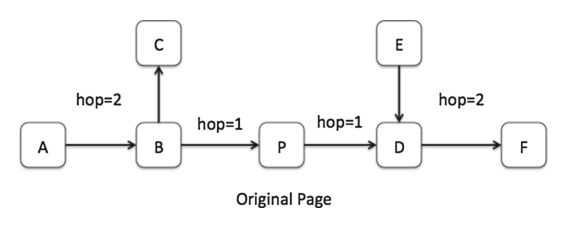
\includegraphics[scale=0.95]{Figures/GenreSim_Draw.eps}
		\caption{GenreSim page selection diagram, found in  \parencite{zhu2016exploiting}.}
		\label{fiig:GenreSim_Draw}
	\end{center}
\end{figure}

GenreSim is a ranking algorithm based on PageSim algorithm, extended to fit in the problem of genre-taxonomy. Similarly to all this kind of algorithms, is based on the assumption where the more webpages refereed to a particular webpage the more this page is related to them in class of topic and/or genre taxonomy. Respectively to the genre-taxonomy the assumption for the GenreSim algorithm this relation is expended to the level of \textit{forward} $F(p)$ and \textit{backwards} $B(p)$ related URL links. Moreover, the web-pages URL structure is also scored and the pages are characterized as \textit{Hubs} $H(p)$ ans \textit{Authorities} $A(p)$. The null hypothesis of the algorithm is than web pages of the same genre are inter-connected with their URL links, thus as small network of a few pages backwards and forwards to a specific web-page consists a "small" network of the same genre. Thus, using the textual and partially the structural information of these selected neighbour pages will amplify the information required to classify this page to the proper genre.

Particularly Hubs are pages with many outgoing URLs, whereas pages with many URLs pointing to the are called authorities. The number of incoming and outgoing URLs are increasing the respective scores as shown in equation \ref{eq:GenreSim_hub_authortities}. However, web-pages with high score but with \textit{few backward URL links} its high likely to be "spam" pages in the context of genre relation. In order to regulate this the $\omega(p)$ factor is intruded of equation \ref{eq:GenreSim_omega}, where is reducing the score for the web pages with few backward links, where is also normalizing the "few links" issue. That is the number of the backward links is correlated to the number of links the page it self is containing. 

\begin{equation}\label{eq:GenreSim_hub_authortities}
	\begin{array}{l}
		H(p) = \sum_{u \in V|p \to u} \omega(p) A(u) \\  
    	A(p) = \sum_{v \in V|v \to v} \omega(p) H(u) \\
    \end{array}
\end{equation}
\begin{equation}\label{eq:GenreSim_omega}
	\omega(p) = \frac{N}{|\log N - \log N(p) | + 1} 
\end{equation}
Therefore for a random webpage in the $G$ graph of web-pages, its score is calculated by equation \ref{eq:GenreSim_Score}. In general the \textit{genre-selection recommendation score} is propagated to the graph path $P(u,v)$ as indicated by the $Score(u, v)$ function of equation \ref{eq:GenreSim_Path}. Thus the recommended webpage's score to be selected is decreasing gradually as the recommended pages is farther (in hops) from the web-page to be classified. The $d$ factor is set to be $0.5$, i.e. the page score is decreasing by half for every hop farther from the page under evaluation. 

\begin{equation}\label{eq:GenreSim_Score}
	Score(p) = H(p) + A(p)
\end{equation}

\begin{equation}\label{eq:GenreSim_Path}
	Score(u, v) =
      \begin{cases}
      	\sum_{p \in P(u, v)} \frac{d Score(u)}{\prod_{x \in p, x  \neq v} (|F(x)| +|B(x)|)}, & v \neq u \\
        Score(u), & v = u \\ 
       \end{cases}
\end{equation}
Finally, the similarity of the candidate neighbour pages to the one under evaluation is calculated form equation \ref{eq:GenreSim_Selection_Score}, which is the ration of the min and the max paths-score sums of all the possible paths, backwards and forwards, to the page under evaluation.

\begin{equation}\label{eq:GenreSim_Selection_Score}
	Sim(u, v) = \frac{\sum_{i=1}^{n} min(Score(v_{i}, u), Score(v_{i}, v))}{\sum_{i=1}^{n} man(Score(v_{i}, u), Score(v_{i}, v))}
\end{equation}
GenreSim is combined with an ML algorithm called MCC (Multiple Classifier Combination). Particularly GenreSim utility is to select a set of webpages where their content (textual and structural) will be used in combination to the "on-page" content as an input to the MCC algorithm for classification of a random webpage to a Genre-taxonomy.

The MCC algorithm is a set of SVM classifiers where each is trained to a particular set of features from the webpage and its neighbours, well selected from the GenreSim, webpages. Then a Decision Template, shown in equation \ref{}, is build and used for the classification of random webpage. Then the Min, Max or Mid values for the classification decision from the matrix are selected for making the final decision for the Genre class of the web-page.

\begin{equation}\label{eq:GenreSim_DP}
	DP(p) = \left(
    	\begin{array}{ccc}
        	d_{11} (p) & \cdots & d_{1|G|} (p) \\
            d_{21} (p) & \cdots  & d_{2|G|} (p) \\
            & \vdots & \\
            d_{N1} (p) & \cdots  & d_{N|G|} (p) \\
         \end{array}
\right)
\end{equation}
Where $|G|$ is the number of genres in a genre taxonomy and the calcification methods is under a closed set setup with $N$ indented (one for each feature set) \textit{SVM multi-class classifier}. 

\section{Focused Crawlers for Genres}\label{chap:relevant_work:sec:intro}

\section{Genres Utility}\label{chap:relevant_work:sec:intro}
journalism historians
Genres variations on students writing...

An other study related to the utility of the genre taxonomy of the \textit{Search Engines Results (SER} is one conducted at Pittsburgh, USA, University.  The experiment measured the correlation of the website's/web-page's genre and the user's preference for completing the task of finding health care information for Multiple Sclerosis and Weight Loss. The results clearly show that the user's task would be significantly easier if the web resource were organized based on their genre and no only on their topic relation ranking \parencite{chi2018sources}.

An other TEXT-GENRE identification utility is for video (e.g. movies, TV series, etc) classification in video/cinematographic genres using the text available such as the subtitles. In this study a variety of ML algorithms has been tested such as SVM, Naive Bayes, Random Forest, Decision Trees and several types of features. Features usually called superficial here where called \textit{content-free} and the ones related to specific words called \textit{content-specific}\parencite{lee2017text}.

\section{Web Genre Temporal Property}\label{chap:relevant_work:sec:intro}
Onnan (Le Tourk de Malakas)
The temporal idiosyncrasy is also an major  

Moreover the  and the context of the text and \textit{the groups defining, forming, and using the genre tag/category}.

Related to the web genre-types, in the very early studies it has been pointed out that the users are the most important component of the research. 

An other study advocating in the temporal manner of the web-genre is the one of  \parencite{caple2017genre} where they show how News web-genre changed overtime and additionally new sub-genres potentially occurred.



\section{Deep Learning Vocabulary of Distributional Features for WGI and WGC}\label{chap:relevant_work:sec:intro}


PRIMITIVE DISTRIBUTIONAL \parencite{kim2010formulating} 


The state-of-the-art in the text-genre classification and WGI/WGC is the Vocabulary-Learning ans particularly the use of the deep-learning methods for building comprehensive-abstract-term vocabularies. This methods due to the nature of the Neural-Networks, mainly used,  the procedure for building vocabulary-models is implicitly embedding a variate of information syntactical, morphological or even structural. However there are some efforts where an explicit use of this kind of information use exploited for the classification task. 

A combination of BOW, superficial and syntactical features. \textit{Content-free} (a.ka. superficial) features in combination with specific words called \textit{content-specific} has been test for genre classification. These feature have been used as an input to a variety of learners such as SVM, Random Forests, Decision trees, Naive Bayes etc with significantly high performance. However, they found that the combination of the features was more efficient when it was combined using a meta-classifier than using a \textit{supervector} containing a sequence of all the features together. Particularly, the where training a different learning for a different set of features and then they were fiddling the results to meta-learner\parencite{lee2017text}.

Their method resembles the deep-learning method of building a DF vocabulary model where afterwords its output is fed to an other classifier. However, this methods can be characterized as Explicate Vocabulary Modeling (EVM) compare to the implicate vocabulary modeling (IVM) when deep learning methods are used.

There are some pros and cons comparing EVM methods to IVM. The main advantage of the "explicit" methods is that they enabling us to figure out which part of the information was really important thus to reduce the computational effort by removing the prepossess of information that is redundant or even causing confusing. On the other hand we have explicitly have to figure out which information to capture, while in the IVM there is no such a need. (THINK THIS STATEMENT AGAIN)

In their study compared their method to in both cases of \textit{binary} and \textit{tf (term frequency)} (Kanaris-Stamatatos)
....
....
....
The state-of-the art relate to the Word-Vectors Learning Models, i.e. the \textit{Deep Learning (Neural Based Models)} or \textit{Pointwize Mutual Information (PMI)}, is the Post-processing of the resulting modeled vectors. Such example is the \textit{unsupervised Post-processing via Conceptors (or Conceptor Negation)}. The main concept is to suppress the outages frequencies using PCA, SVD and most recently Conceptors Negation. The latest is a methodology (unsupervised) of Conceptors are a family of regularized identity maps introduced by (Jaeger 2014 ???) where a linear transformation is taking place minimizing a loss function similar to the PCA process. However, this methodology on the contrary to the PCA is a "Soft" regularization or "Soft" noise filtering, while PCA is considered "Hard". In both cases by projecting the data-point to the prediction space we are able to filter the noise or outages samples. Intuitively, these methods are post-processing the distributional feature vectors in order to enrich their semantic content. Moreover, using the "soft" noise reduction filtering (CITE Unsupervised Post-processing of Word Vectors via Conceptor Negation ).

Then \textit{n-gram term types} for WPGC problem proposed by a series of papers by Manson et al.\parencite{mason2009n,mason2009classifying,mason2009distance}. In their studies were comparing their method to previous studies on WPGC based on n-grams and they have tested their approach on the range of 2-grams to 10-grams. The learning models under comparison was SVM, k-Nearest Neighbors, and a distance based method they proposed. Their approach uses a distance measure from the domain of \textit{Author Identification} and they used this measure with three different representation of the genre classes. In oder to form the a prediction class, using this their method, were getting the vectors of the training sample and forming a centroid(characteristic) vector. Then an arbitrary web page vector were compared to the characteristic vector with the distance measure in order to be classified. Their approach was comparable to other methods, however, SVM had shown better performance. In their work studied two methods of selecting the genre features for discriminating the pages, one by keeping an $z$ number of the most frequent features within the genre training corpus. The second feature approach was the use of the \textit{chi-square statistic} ($\chi^{2}$), which performed \textit{statistical significantly} better than \textit{frequency based selection}. It is important to note that their series of works was extensively examined the influence of n-grams size to the performance of the prediction models and they have shown that there is a statistical
significantly difference between the different sizes.

There is an other study from Dong et al.\parencite{dong2006binary} focusing on the measures that could potentially used for feature selection in the context of WPGC. The have tested\textit{ chi-square statistic} ($\chi^{2}$), Information Gain and Mutual Information over three samples sets of three different genres. Each of the evaluation data sets for every genre, was composed from pages related to the genre and random pages. Their experiments were binary classification tasks using Naive Bayes, SVM, and Neural network classifiers. Irrespectivelly of the classifiers all the statistical measures used for feature selection had similarly good performance. The feature size they used was 5, 20 and 100 features, where for 20 and 100 the results had no statistically significant difference. The term vectors or the web pages where binary formatted.


""Examples of word vectors include Word2Vec (Mikolov et al. 2013), GloVe (Pennington, Socher, and Manning 2014), Eigenwords (Dhillon, Foster,and Ungar 2015), and Fasttext (Bojanowski et al. 2017). These word vectors are usually referred to as distributional word vectors, as their training methods rely on the distributional hypothesis of semantics (Firth 1957)."""


\section{Using the Web as a Corpus - The Genre Approach}\label{chap:relevant_work:sec:intro}

\section{Genre Research outside pure CS (???)}\label{chap:relevant_work:sec:intro}


\section{The Web Genre units: Section, Page, Site}

In all studies it was pointed out that in most cases in a webpages or in a text usually there are multiple genres.... \parencite{lee2017text} (also Ashegi, Santini, and other old citations).


\section{Web Genre Corpora: An unfinished work in progress}\label{chap:relevant_work:sec:intro}

The constitution process for the rules required to be followed for composing a text corpus is still a research problem in \textit{linguistics studies}, while the utility of the genre-taxonomy is vividly pointed out. A collection of texts cannot be assumed to be a corpus by default due to several issues should be considered starting with the taxonomy definition where mostly is an overlapping problem, then the texts should have several properties linguistically and statistically defined. The homogeneity in temporal manner, whether are from multiple languages and the way have been collected; \textit{speech, spoken or written corpus}. Particularly speech corpus implies voice recording while spoken means to be transcribed from speech samples. Particularly for the genre-taxonomy the homogeneity related to the time samples has been collected is very critical since the genres are changing over time until a new genre occurs replacing or dividing from an older \parencite{dash2018history}. Blogs, for example, was the evolution of "personal/memory diaries" when they became public on the web and named "web-logs" then in a second time evolution renamed to "blogs" where their content also changed now is mostly like an \textit{informal journalism} rather than a diary.

The NLP community has overcome, by ignoring mostly, the problem of a non-well established corpus of the WGI, and in general for the \textit{Text Genre Identification}. There are at least tree publication on the effort on \textit{corpus building methodologies} with vividly different approaches, yet the problem is remaining open due to several issues described in detail in section
\ref{chap:relevant_work:sec:linguistics_definition} and in \parencite{melissourgou2017genre,asheghi2014semi (Ashegi,2018_Book_HistoryFeaturesAndTypologyOfLa_WEB_TEXT_CORPUS.pdf). 

All the approaches are focusing on the genre's main principals, i.e. the function, form and communicative purpose. While in \cite{asheghi2014semi} the focus was on the semi-automated evaluation procedure in the categorization of the texts, in \parencite{melissourgou2017genre} the process is focusing on the systematic manual process.  This process is based on a well established theory of  the Systemic Functional Linguistic (STL) framework where as a shortcut in the process can help on building and evaluating a genre taxonomy corpus. 

There is no drought for the significant contribution of the above studies where all three can be used as the solid framework for building \textit{web-genre-taxonomy corpora} and web-text corpora in general. The utility of the each work can be used as multi-layer filtering process:  1) starting with the automated crawling of the web using focused crawling as explained above \ref{}, 2) Using non-experts crowd-sourcing semi-automated procedures form first level filtering, 3) using the methodology of manual STL based evaluation for fast qualitative analysis and categorization of the post-crowdsourcing-filtered corpus. 

Starting form the final step \parencite{melissourgou2017genre} work firstly is resolving the ambiguity on the notions related to genre. As they explained the terms "genre", "register", and "text type" are used interchangeably, complimentary and even contradictory, plus to the debate related to the terms usage. However, in general there terms it turns out to be subsets and super-sets of one to the other. Particularly \textit{text's register, communicative purpose, form} are all components of the \textit{text's genre}, while \textit{text type} is mainly defined by the \textit{text's form}. Alternatively, register is used to describe very general concepts of writing styles such as \textit{formal/informal} while genre mostly includes also the purpose such as \textit{news/blog}, where news' style is mostly formal and blog's infomal. Moreover, text's form is also one of the three components of the \textit{register} where then is called "mode". One could attempt to describe the connection of these terms in a mathematical equations such as in eq.  

\begin{equation}\label{eq:genre_notion_in_math}
	G  \subseteq P \uplus F \uplus T \uplus M
\end{equation}
where $G$ is the genre, $P$ is the communicative purpose and $F, T, M$ are the "register's" components. $F$ is the \textit{field} which answers to the question of \textit{Why?} the text was composed. $T$ is the \textit{tenor} which answers the question of \textit{Who?} or/and to \textit{Whom?} the text was written. $M$ is the \textit{mode} which is the text's form. Note, that G is not exactly equal to their sum of these components of the text, because, as it has also mentioned before in this thesis although the text's context we would like to be orthogonal to the genre - since is mostly related to the topic - yet there are some contextual text peaces that are critical for the genre identification, exactly as it was happening in the cognitive experiments on genre identification of \parencite{clark2014you, lieungnapar2017genre} (briefly explained in section \ref{chap:relevant_work:sec:linguistics_definition}).

An other interesting path towards to the process automating the building of Genre-Taxonomy corpora is the one found in \parencite{lieungnapar2017genre}. They are using a simple K-means clustering method for finding an automated procedure for capturing the possible correlation of \textit{logistic features} and the \textit{Popular Science Sub-Genres}. In their methodology they are using set of manually extracted linguistic features as presented in table \ref{chap:relevant_work:tbl:pop_science_features} and then they are correlating the z-scores of these features to the possible 4 clusters found to be in the Popular Science \textit{web documents}. Following the same strategy they have managed to show the correlation of the sub-genres to the science disciplines and document sources. Finally they have managed to correlate manually identified genre's function to the linguistic features. Showing that it is possible by using a short of \textit{Funnel like Filter} is possible to gradually extract higher and more abstract levels of information starting with the linguistic features, conginuing with function features (or text-registers) (e.g. Impersonal, Narrative, Persuasive, Informative, Elaborated, Impersonal) and finally classifying the genres. Finally, they have shown that their final evaluation to their, obviously, semi-automated process was as good as the experts agreement on the same task after they have manged to form a "golden standard" manually. 




\section{Discussion}

AGI/AGC and particularly WGI is a complex problem for NLP ( and in computational linguistics in general) where several approaches has been proposed in the effort to tackle this task. All the above faceted survey giving us a fruitfully information set where we should put it into an order and derive a conclusion where it could help the AGI research to go several steps forward. Particularly here it is assumed that eventually the linguistic research will converge to the NLP in the direction of creating rich genre-taxonomy corpora by using semi-automated methods and most importantly a well defined methodology to assess and constitute them properly. Thus by overcoming this bottle neck here it is discussed the potential directions for the AGI task.

Feature selection and document representation independently or combined with the classification/identification ML method seem to be the main problem most of the researchers are primarily trying to tackle. In section \ref{chap:relevant_work:sec:features} there is a great amount of work on heuristic methods for capturing the amount of information for enabling any out-of-the box ML method (or special version of it) to identify the genres of a genre-taxonomy. The whole effort of more than a decade on the feature selection leading as in two main conclusions. The \textit{power of words} and the \textit{language dependency}.

The power of words, in the sense that in all the cases of (see tables .....) it seems than there are words with a great "informative energy" and they can even define the genre when they are present on the URL of the web page (see work of identify web-genre using URL). In addition there are cases where this words although they are tightly connected to the context they are indicators also for genre-identification (see study for POP-Science sub-genres). Finally, using DF features it seems again that words are good enough for returning all the information required for the AGI task. 

On the other hand sine the words are so powerful they are tightly connected to the language where the text is written. Thus all these ML automated proposals are potentially canceled when the language is written. Moreover, superficial text information, such as colon frequency, document length, sentence mean length, and single-sentence paragraph count, seems to work fine in cases of cross-lingual genre classification such as in the case of \parencite{nguyen2019cross}. 

To this end in feature selection and document representation the research seem to be  required to focusing in generalized representations not necessarily superficial based but mostly in feature selection methods where they can be used in any language and ideally cross-lingual. Again DF features seems one of the research paths one could be follow for the AGI.

Based on the DF features paradigm \textit{sampling in several text properties} in character, word, paragraph, text level seems to be a path to follow especially in a case where an ML algorithm could do that as a part of the its whole optimization procedure, from the raw text.

The ML methods experimental framework in respect of closed-set and open-set is an other very import aspect for the AGI....


























%!TeX spellcheck = en-US

\chapter{Open-set and Closed-Set Classification for WGI}

\label{chap:relevant_work}

%----------------------------------------------------------------------------------------

% Define some commands to keep the formatting separated from the content
\newcommand{\keyword}[1]{\textbf{#1}}
\newcommand{\tabhead}[1]{\textbf{#1}}
\newcommand{\code}[1]{\texttt{#1}}
\newcommand{\file}[1]{\texttt{\bfseries#1}}
\newcommand{\option}[1]{\texttt{\itshape#1}}

%----------------------------------------------------------------------------------------

\section{Introduction}\label{chap:relevant_work:sec:intro}

\subsection{One-Class Classification\label{subsec:One-Class-Classification}}

The main difference of the One Class Classification problem (OCC) with respect to the conventional multi-class or binary classification problem is that in OCC there are only available positive examples of a class and none or very few negative examples. There are several approaches towards the solution of this problem. A compact survey on OCC is provided by Khan et al.\cite{khan2010survey}. In this section, we present a brief review of the OCC methods used for Document Classification (DC) and Information Retrieval (IR). We mainly consider SVM-based OCC methods.

To begin with there are several references to the well known Scholkopf et al.\cite{scholkopf1999estimating} \textit{which actually presents an alternative solution to the problem of the overlapping distributions of samples, known as }$\nu$-SVM \cite{bishop2006}. The nature of $\nu$-SVM is allowing us to use it effortless in Binary Classification problems as long as to OCC problems. This is owing to parameter $\nu$ which is both controlling the fraction of SVs and the \textit{margin errors, i.e. point of the positive sample considered as outliers. }In the case of One-Class SVM (OC-SVM) the optimization process begins with considering, as the only negative example, \textit{the origin }of the vector space\textit{, }defined from the \textit{data space. }Some more details for OC-SVM is given into the section \ref{subsec:One-Class-SVM-Model}.

OC-SVM model has been used in DC, where only positive example were available. Building upon OC-SVM concept Manevitz and Yousef \cite{manevitz2002one,khan2010survey}have been build an OCC SVM model, called Outliers-SVM, that takes into account a few more points, other that \textit{the origin}, from the positive sample as outliers for achieving a similar model to the one of Scholkopf et al. The idea of outliers-SVM is to define a model of measurement for measuring the distance of some points, in the positive sample space, where it will treated as \textit{Outliers,} additional to the origin of the data space. In their outliers-SVM they have used \textit{Hamming distance} as the model of measurement. However, while comparing their model (Outliers-SVM) to One-Class SVM, One Class Neural Networks, One Class Naive Bayes Classifier, One Class Nearest Neighbor, and Rocchio Prototype, One-Class SVM has higher or at least comparable performance to all the others. In addition they have pointed out that One-Class SVM it seems to be sensitive to the Term-Vector formats - i.e. \textit{binary, tf, tf-id, etc.} - and sensitive to the amount of features (i.e. dimensions) that have been kept.

The Prototype or Rocchio's algorithm was used for IR problems because of its simplicity and consistency \cite{joachims1997probabilistic}. The learning process for this method is just to add all the vectors of the training set in to one \textit{prototype vector}. An arbitrary vector is classified as positive or negative using the angular distance from the prototype vector and a threshold. In this method term-vectors are having tf-idf format. 

Datta (cited in \cite{manevitz2002one}) proposed Naive Bayes Classifier modification for OCC problems and use only positive samples in the learning process. The prediction model induced in this case is a \textit{probability density function} of a class $E$. Classifying the a document $d$ involves calculating the probability of the document $p(d|E)$ which is equal to the product of its features $w_{n}$ probabilities $p(w|E)$, where $n$ is the number of document's feature/term-vector. To decide weather of not the document is classified as positive its required
a threshold. 

In OC-SVM and few other OCC method the process of model optimization requires only \textit{positive sample} points and no \textit{negative} or \textit{unlabeled examples}. Thus building process it is not taking into account information that might be useful from even a poor negative sample (if any available) or a set of unlabeled data, vastly available. However, there are some OCC methods exploiting the availability of \textit{unlabeled data} for building an classification models, where some of them have been evaluated in the context of IR and DC. 

Yu proposed two OCC algorithms that use positive and unlabeled data for building a classification model that describes the \textit{single class boundary} \cite{yu2005single}. Their \textit{Mapping Convergence }(MC) algorithm is incrementally labeling negative data from an \textit{unlabeled data set} using the margin maximization property of SVM, while \textit{Support Vector Mapping Convergence} (SVMC) was their second proposed algorithm which optimizes the MC algorithm for fast training. Both of their algorithms had been compared into a real world text classification, letter recognition, and diagnosis of breast cancer. Additionally MC and SVMC had been compared to OC-SVM, Spy Expectation Maximization (S-EM), SVM-NN (i.e. C-SVM using unlabeled data point as negative ones) and Naive Bayes with Noisy Negatives. Above all models SVMC (and MC) performance was significantly better to all the other models, while OC-SVM was the second best in performance. In Yu's paper there are pointed out the difficulties of OCC which are referred briefly in section \ref{subsec:One-Class-SVM-Model}.

Spy EM (Spy EM) is an other method using unlabeled data in the training procedure and it had been tested in DC domain. The procedure proposed in Liu et al.\cite{liu2002partially}, involves the \textit{Naive Bayesian Classification} with \textit{Expectation maximization algorithm}. This method has several limitations such as the assumption of attribute independence which results in linear separation, and the requirement to estimate the proper prior probabilities which is difficult task \cite{yu2005single}.

An alternative \textit{two-step} method like S-EM proposed by Li and Liu \cite{li2003learning}. Again they have pointed out that their `OCC method, like the other OCC methos, need a large positive data `sample and negative samples derived from unlabeled data to induce `a ``good'' classifier.

To conclued, in all OCC publication cited in this paper it had been point out that the problems encountered when using conventional classificaiton models such as the curse of dimensionality, the generalization of the method, etc., it seems to be amplified when in OCC methods. In all the OCC models it has been reported that the problem is the difficulty to decide how tightly should be the boundary that contours the positive data, additional to the problem of the attribute selection which will be used for finding the outliers or the automated formation of a \textit{negative body of samples}. Hence, the performance of OC-SVM should be expected to be poorer comparing to \textit{binary }or \textit{multi-class} classification SVM\cite{khan2010survey,manevitz2002one,yu2005single,scholkopf1999estimating,li2003learning}.

%!TeX spellcheck = en-US

%\chapter{Evaluation Methodology for WGI and Computational Text Categorization}
\chapter{Evaluation framework for open-set WGI}

\label{chap:eval_methods}

%----------------------------------------------------------------------------------------

% Define some commands to keep the formatting separated from the content
\newcommand{\keyword}[1]{\textbf{#1}}
\newcommand{\tabhead}[1]{\textbf{#1}}
\newcommand{\code}[1]{\texttt{#1}}
\newcommand{\file}[1]{\texttt{\bfseries#1}}
\newcommand{\option}[1]{\texttt{\itshape#1}}

%----------------------------------------------------------------------------------------

\section{Introduction}\label{chap:eval_methods:sec:intro}

This chapter is describing the evaluation metrics required for the open-set WGI task. Particularly it is shown with simple examples the effect of the a measurement methods to the evaluation results and the misleading conclusions on can have when the wrong measurement method is adopted. Moreover some evaluation measures are presented specialized for the open-set framework where recently have been discover and adopted for several domains inside and outside the \tetxit{text minminng} domain.

The standard evaluation approach is to use a previously well tested evaluation methodology and measures. However, the closed-set measures is later shown that they are not proper for the open-set framework in their standard form. 

To reason it in few words the problem is that these measures are based on the \tetxit{Confusion Matrix} which can capture only two condition per variable. However, in the case of open-set framework there is one say "global" condition where all the variables of the table drops. This condition is occurring when the \tetxit{rejection condition of the open-set algorithm is trigered. That is when an open-set algorithm responds "I don't know" for an arbitrary sample. 

As expled in chapter \ref{chap:openset} there are some effortes to crate open-set algorithms than could model the \tetxit{unkown} or \textit{unstructured noise} samples. In this case it could be possible the out-of-the-box closed-set evaluation methods be sufficent,however, in most ML algorithms where a rejection critirion is considered this is nearly imposible as it will be presented later.

\section{Closed-set vs Open-set Measures}\label{chap:eval_methods:sec:measures} 

In this section it is presented how the text mining evaluation measures are affected by the type of the by the type of the task's approach scenario. That is, whether i
t is an open-set of closed-set classification framework.

Starting with the \textit{Confusion matrix} where the basic closed-set evaluation measures are based it is shown the diffence in measure of the Precision and Macro-Precision diffence (also for Recall) in the open-set framework. Moreover, it is shown how these measures are affected by he openness score which is the score for evaluating the difficulty level of an open-set problem.

Finally, the \tetxit{Open Space Risck} is presented which is the measure helping an open-set algorithm to regulate the potentially error in the presense of \tetxit{noise} in the testing or/and \tetxit{outages} in the training phase.


\subsection{Confusion Matrix and $F$ Score}\label{chap:eval_methods:sec:prf_micro}

In Machine Learning (and Statistical) Classification, a \textit{Confusion Matrix} is a table that depicts the performance of an algorithm. It is a special case of a \textit{Contingency Table}, with two dimensions, actual and predicted classes. Thus, in the a binary case such as in the table \ref{chap:eval_methods:tbl:bin_confusion}, there are for cases occuring. True Positive (TP), True Negative (TN), False Postive (FP), False Negative (FN).

In the case of binary classification the sampels under the class distribution A are desired, i.e. positive, and all the other samples outside the distribution are considered negative, classified in say class B. Then TP and TN are the counts of samples predicted corectly under the a class A (positive) or class B (negative). Therefore, the FP and FN are the samples a binary algorithm missleaded and predicted the wrong class. 

\begin{table}[H]
	\center
	\caption{Confusion matric of binary classification}\label{chap:eval_methods:tbl:bin_confusion}
	\begin{tabular}{c c c c c}
		& & \multicolumn{2}{c}{Actual} & \\
		\cline{3-4}
		\multirow{3}{*}{\rotatebox[origin=r]{90}{Predicted}} & & \multicolumn{1}{|c}{A} & \multicolumn{1}{c|}{B} & \\
		\cline{2-4}
		& \multicolumn{1}{|c}{A} & \multicolumn{1}{|c}{\textbf{50}} & \multicolumn{1}{c|}{25} & 75 \\
		& \multicolumn{1}{|c}{B} & \multicolumn{1}{|c}{20} & \multicolumn{1}{c|}{\textbf{45}} & 65 \\
		\cline{2-4}
		&  & 70 & 70 & \textbf{95}\\
	\end{tabular}
\end{table}

In order to measure the performance a binary classification algorithm the \tetxit{Accuracy} is a common measure which is actually the ration of all the correct prediction overall the predictions (which is equivalent to the number of the samples of the whole data set). Formally, it is shown in the equation \ref{chap:eval_methods:eq:accuracy} and for the example of the table \ref{chap:eval_methods:tbl:bin_confusion} its value is $A = 95/140 = 0.68$

\begin{equation}\label{chap:eval_methods:eq:accuracy}
A = \frac {TP + TN} {TP +  TN + FP + FN}
\end{equation}

However, one can get a better insight when it is measured the algorithms ability distinguishing the samples which they are under the distribution it has been trained for. Moreover, to be measured its ability of recognizing the samples of this distribution. The former is called \tetxit{Precision} and the second it is called \tetxit{Recall} and their formal expressions are in equation \ref{chap:eval_methods:eq:precision} and \ref{chap:eval_methods:eq:recall} respectively. 

\begin{equation}\label{chap:eval_methods:eq:precision}
	P = \frac {TP} {TP + FP}
\end{equation}

\begin{equation}\label{chap:eval_methods:eq:recall}
	R = \frac {TP} {TP + FN}
\end{equation}

\tetxit{Precision} is also known as \tetxit{Positive Predictive Value (PPV)}. \textit{Recall} is also known as \textit{Sensitivity, Hit Rate and True Positive Rate (TPR)}. 

Second multiclass with 7 var closed set

third multiclass open set 





\subsection{Macro-Precision and Macro-Recall}\label{chap:eval_methods:sec:prf_macro}



\subsection{PRC and ROC Curves}\label{chap:eval_methods:sec:roc_prc}



\section{Area Under the Curve (AUC)}\label{chap:eval_methods:sec:closed_set_classification} 

Precision-Recall curve is a standard method to visualize the performance of classifiers. In this paper, the Precision-Recall curve is calculated in 11-standard recall levels $[0,0.1,...,1.0]$. Precision values are interpolated based on the following formula:

\begin{equation}
	P(r_j)=max_{r_j \leqslant r \leqslant r_{j+1}}(P(r))
\end{equation}

\noindent
where $P(r_j)$ is the precision at $r_j$ standard recall level.


To compensate the potentially unbalanced distribution of web pages over the genres, we are using the macro-averaged precision and recall measures. In more detail, we use the modified version of precision and recall for open-set classification tasks proposed by \parencite{mendesjunior2016}. This modification calculates precision and recall only for the known classes (available in the training phase) while the unknown samples (belonging to classes not available during training) affect false positives and false negatives. To find parameter settings that obtain optimal evaluation performances we use 2 scalar measures, the Area Under the Precision-Recall Curve (AUC)and $F_{1}$. We will show that the appropriate selection of the optimization measure is highly significant in the presence of noise.


\section{Re-defining the Open Space Risk}\label{chap:eval_methods:sec:open_space_risk} 

The open space risk in \parencite{scheirer2013toward} is originally defined as in eq. \ref{chap:eval_methods:eq:the_original_open_space_risk}

\begin{equation}\label{chap:eval_methods:eq:the_original_open_space_risk}
	R_{o}(f) = \frac{\int_{o} f_{y}(x) dx}{\int{S_{o}}  f_{y}(x) dx}

\end{equation}

\noindent
where $R_{o}(.)$ is the open-space risk function and $f_{y}(x)  \in \{0, 1\}$ is the classification function of class $y$, where $1$ is for recognizing its class and $0$ when not. $S_{o}$ is the large hyper-sphere where all the positive training data points and the \textit{positive open space area} $O$. 

The original formulation of the eq. \ref{chap:eval_methods:eq:the_original_open_space_risk} $O$ area cannot be constrained by any means. The only information we are getting is the farther form the training date we go the risk of miss-classification is increasing One method to constrain the problem is by using the center of the positively labeled training data and defining a radios $r_{o}$ where it will reduce the open space area based on the positively labeled empirically observations. Then the $O$ is defined by the equation eq. \ref{chap:eval_methods:eq:openspace_spherical_constrained}

\begin{equation}\label{chap:eval_methods:eq:openspace_spherical_constrained}
	O = S_{o} - B_{r_{y}}(C_{y})
\end{equation}

\noindent
where $B_{r_{y}}(.)$ is the function which defines the area of radius $r_{y}$ of the $C_{y}$ class defined by its training data \parencite{fei2016breaking}.

\section{Openness test}\label{chap:eval_methods:sec:open_space_risk}

In \parencite{scheirer2013toward} work in image processing, the \textit{openness measure} is introduced, as shown in eq. \ref{chap:eval_methods:eq:openness}. The openness measure indicates properties of an open-set classification task by taking into account the number of \textit{training classes}, i.e. the known labels used in the training phase and the number of \textit{testing classes}, i.e., the labels, both known and unknown, used in the testing phase.

\begin{equation}\label{chap:eval_methods:eq:openness}
	openness=1-\sqrt{\frac{ | Training Classes | }{ |Testing Classes | }}
\end{equation}

When openness is $0.0$, it is essentially a closed-set task, that is the training and testing classes are the same or there is no noise. When openness reaches $1.0$ this means that the known classes are far less than the unknown classes, that is the amount of noise is especially high. Therefore, by varying the openness level we can study the performance of WGI models in different conditions.

Note that the openness measure can only be applied to corpora where all available documents have been labeled with genre information. In other words, we have to know the genre labels of the pages that form the noise (i.e. structured noise). Thus, it cannot be applied to SANTINIS corpus where the web pages taken from the SPIRIT collection are unclassified (i.e., unstructured noise). On the other hand, the SANTINIS corpus provides the opportunity to examine WGI performance when all documents not belonging to the known labels are grouped into one single (highly heterogeneous) class.



\section{Domain Transfer Measure}\label{chap:eval_methods:sec:domain_transfer_measure}

A practical methodology for evaluating a classification/identification ML model in a text-categorization task is the \textit{Domain Transfer Evaluation}. The goal of this evaluation methodology is to measure the generalization of the model when training corpus is rather small and to evaluate how the model would perform in an unknown domain for the same task. 

Particularly for the AGI/WGI with this measure we can evaluate a ML algorithm when for example the model has been trained to identify \textit{News} and \textit{Wiki} genres, however, the available corpus would be only from \textit{Technology products Topics}. Then by testing it on {Sports Topics} we could evaluate the model in such a case when very small corpus is available for training. In addition using this methodology we can evaluate the models behavior depending on the \textit{Features} have been selected for the training, e.g. BOW, POS, Term N-grams etc. 

One can measure the performance, say Accuracy, F1-statistic, Precision-Recall Curve,  Receiver Operating Characteristic (ROC) Curve etc, and then compare the two measures pairwise for every domain combination (e.g. $\{Mobile Phones, Football\}$, etc). However, it would be easier to have measure for all possible combinations training/testing of different domain combinations. 

The measure proposed from \parencite{finn2006learning} and shown in equation \ref{eq:gnr_dom_transit_general} in its generalized form. Originally, this measure was designed for Accuracy measure in mind. However, it can be used for any measure say $F_{1}$-statistic in order to fit in open-set framework and not respected to the closed-set also (Να ελέγξω αν το Accuracy μπορεί να χρησιμοποιηθεί για Open-set). 

\begin{equation} \label{chap:eval_methods:eq:office_doc_ensemble}
	T^{C,F} = \frac{1}{N(N-1)} \sum_{A=1}^{N} \sum_{B, \forall B \neq A}^{N} \left(  \frac{M^{C,F}_{A,B}}{M^{C,F}_{A,A}} \right)
	\end{equation}

	\noindent	
where T is the \textit{Transfer Measure Score}, M is the measure of choice (Accuracy, $F_1$, Precision, Recall, etc), F is the \textit{Feature Set}, and C is the \textit{Genre Class}. 

























%!TeX spellcheck = en-US

\chapter{Handling the Noise of the Web-Genres}

\label{chap:noise}

%----------------------------------------------------------------------------------------

% Define some commands to keep the formatting separated from the content
\newcommand{\keyword}[1]{\textbf{#1}}
\newcommand{\tabhead}[1]{\textbf{#1}}
\newcommand{\code}[1]{\texttt{#1}}
\newcommand{\file}[1]{\texttt{\bfseries#1}}
\newcommand{\option}[1]{\texttt{\itshape#1}}

%----------------------------------------------------------------------------------------

\section{Introduction}\label{chap:noise:sec:intro}

\section{Noise vs Outages on Open-set Classification}\label{chap:noise:sec:noise_vs_outages}

\section{Open-set Framework Evaluation on Noise}\label{chap:noise:sec:openset_evaluation}

%\section{Open-set Ensembles for WGI with Noise}\label{chap:noise:sec:openset_ensembles}

\section{Open-set WGI Methods}\label{sec:Ensembles_Description}



\section{Experimental Setup}\label{sec:experimental_setup}
\subsection{Corpora}\label{sec:corpora}
In this paper we study the performance of the open-set classification models on the WGI task. In particular, the two open-set algorithms described above are analytically tested on benchmark corpora. In particular, our experiments are based on the following corpora already used in previous work in WGI \citep{meyer2004genre,santini2007automatic,kanaris2009learning}:

\begin{enumerate}
\item \textit{SANTINIS} \citep{mehler2010genres_on_web}: This is a corpus comprising 1,400 English web pages evenly distributed into 7 genres as well as 80 BBC web pages evenly categorized into 4 additional genres. In addition, it comprises a random selection of 1,000 English web pages taken from the SPIRIT corpus \citep{joho2004spirit}. The latter can be viewed as noise in this corpus. Details are given in table \ref{tbl:genre_tags}.
\item \textit{KI-04} \citep{meyer2004genre}: This is a collection of 1,205 English web pages unevenly categorized into 8 genres. Details can be seen in table \ref{tbl:genre_tags}.
\end{enumerate}


Our text representation features are based exclusively on textual information from web pages excluding any structural information, URLs, etc. Based on the good results reported in \citep{sharoff2010web,pritsos2013open,Asheghi2015} as well as some preliminary experiments, the following document representation schemes are examined: Character 4-grams (C4G), Word unigrams (W1G), and Word 3-grams (W3G). We use the Term-Frequency (TF) weighting scheme  and the feature space is defined by a \textit{Vocabulary} which is extracted based on the terms appearing at training set only.

As concerns OCSVM model, two parameters have to be tuned: the number of features $F$ and $\nu$. For the former, we used $F=$\textit{\{1k, 5k, 10k, 50k, 90k\}}, of most frequent terms of the vocabulary. Following the reports of previous studies \citep{scholkopf1999estimating} and some preliminary experiments, we examined $\nu$\textit{=\{0.05, 0.07, 0.1, 0.15, 0.17, 0.3, 0.5, 0.7, 0.9\}}. In comparison to \citep{pritsos2013open}, this set of parameter values is more extended. With respect to RFSE, four parameters should be set: the vocabulary size $F$, the number of features used in each iteration $fs$, the number of iterations \textit{I}, and the threshold $\sigma$. We examined $F$\textit{=\{5k, 10k, 50k, 100k\}}, $fs$=\textit{\{1k, 5k, 10k, 50k, 90k\}}, \textit{I}=\textit{\{10, 50, 100\}} (following the suggestion in \citep{koppel2011authorship} that more than 100 iterations does not improve significantly the results) and $\sigma$\textit{=\{0.5, 0.7, 0.9\}} (based on some preliminary tests). Additionally, in this work we are testing three document similarity measures: cosine similarity, MinMax similarity,  and combined cosine similarity and MinMax. Finally, to extract the best possible parameter settings for each classification method we apply grid-search over the space of all parameter value combinations.

\begin{table}
\center
\begin{tabular}{|l|l|l|l|}
\hline
\multicolumn{2}{|c|}{SANTINIS} & \multicolumn{2}{c|}{KI-04}\tabularnewline
\hline
\multicolumn{1}{|c|}{Genre} & \multicolumn{1}{c|}{Pages} & \multicolumn{1}{c|}{Genre} & \multicolumn{1}{c|}{Pages}\tabularnewline
\hline
\multicolumn{1}{|l|}{Blog} & \multicolumn{1}{c|}{200} & \multicolumn{1}{l|}{Article} & \multicolumn{1}{c|}{127}\tabularnewline
\multicolumn{1}{|l|}{Eshop} & \multicolumn{1}{c|}{200} & \multicolumn{1}{l|}{Discussion} & \multicolumn{1}{c|}{127}\tabularnewline
\multicolumn{1}{|l|}{FAQ} & \multicolumn{1}{c|}{200} & \multicolumn{1}{l|}{Download} & \multicolumn{1}{c|}{152}\tabularnewline
\multicolumn{1}{|l|}{Frontpage} & \multicolumn{1}{c|}{200} & \multicolumn{1}{l|}{Help} & \multicolumn{1}{c|}{140}\tabularnewline
\multicolumn{1}{|l|}{Listing} & \multicolumn{1}{c|}{200} & \multicolumn{1}{l|}{Link Collection} & \multicolumn{1}{c|}{208}\tabularnewline
\multicolumn{1}{|l|}{Personal Home Page} & \multicolumn{1}{c|}{200} & \multicolumn{1}{l|}{Portrayal-Non Private} & \multicolumn{1}{c|}{179}\tabularnewline
\multicolumn{1}{|l|}{Search Page} & \multicolumn{1}{c|}{200} & \multicolumn{1}{l|}{Portrayal- Private} & \multicolumn{1}{c|}{131}\tabularnewline
\multicolumn{1}{|l|}{DIY Mini Guide (BBC)} & \multicolumn{1}{c|}{20} & \multicolumn{1}{l|}{Shop} & \multicolumn{1}{c|}{175}\tabularnewline
\multicolumn{1}{|l|}{Editorial (BBC)} & \multicolumn{1}{c|}{20} &  & \tabularnewline
\multicolumn{1}{|l|}{Features (BBC)} & \multicolumn{1}{c|}{20} &  & \tabularnewline
\multicolumn{1}{|l|}{Short Bio (BBC)} & \multicolumn{1}{c|}{20} &  & \tabularnewline
\multicolumn{1}{|l|}{Noise (Spirit1000)} & \multicolumn{1}{c|}{1000} &  & \tabularnewline
\hline
\end{tabular}
\caption {Corpora descriptions and amount of pages per genre.}
\label{tbl:genre_tags}
\end{table}


\section{Experiments}\label{sec:Experiments_Results}
\subsection{WGI with Unstructured Noise}\label{sec:WGI_noise}

We initially examine the performance of OCSVM and RFSE models based on SANTINIS corpus. In the training phase, only the 11 known genres are considered. In the testing phase, the noise pages coming from the SPIRIT corpus are also used. Note that information about the true genre of these pages is not available. Therefore, we have to deal with unstructured noise. We perform  10-fold cross validation and in each fold we include the full set of 1,000 pages of noise. This evaluation strategy is giving a more realistic evaluation framework since the size of the noise is much greater than the size of any genre included in the given palette.

Figures \ref{fig:MacroPRC_OCSVME_W3G_W1G_C4G_OPTIMAL_SANTINIS} and \ref{fig:MacroPRC_RFSE_W3G_W1G_C4G_OPTIMAL_SANTINIS} depict the Precision-Recall curves (PRC) of OCSVM and RFSE models, respectively. For each model and each one of the three document representations, the parameters that maximize performance with respect to the $F_{1}$-measure are used. Note that when recall does not reach 1.0 this means that some pages belonging to known classes were classified as unknown. In all cases, RFSE outperforms OCSVM. Moreover, for both methods, W3G seems to be the best feature type for this corpus, followed by C4G. OCSVM performance is only comparable with RFSE when W3G is used.

\hfill \break


\begin{figure}[H]
\begin{center}
    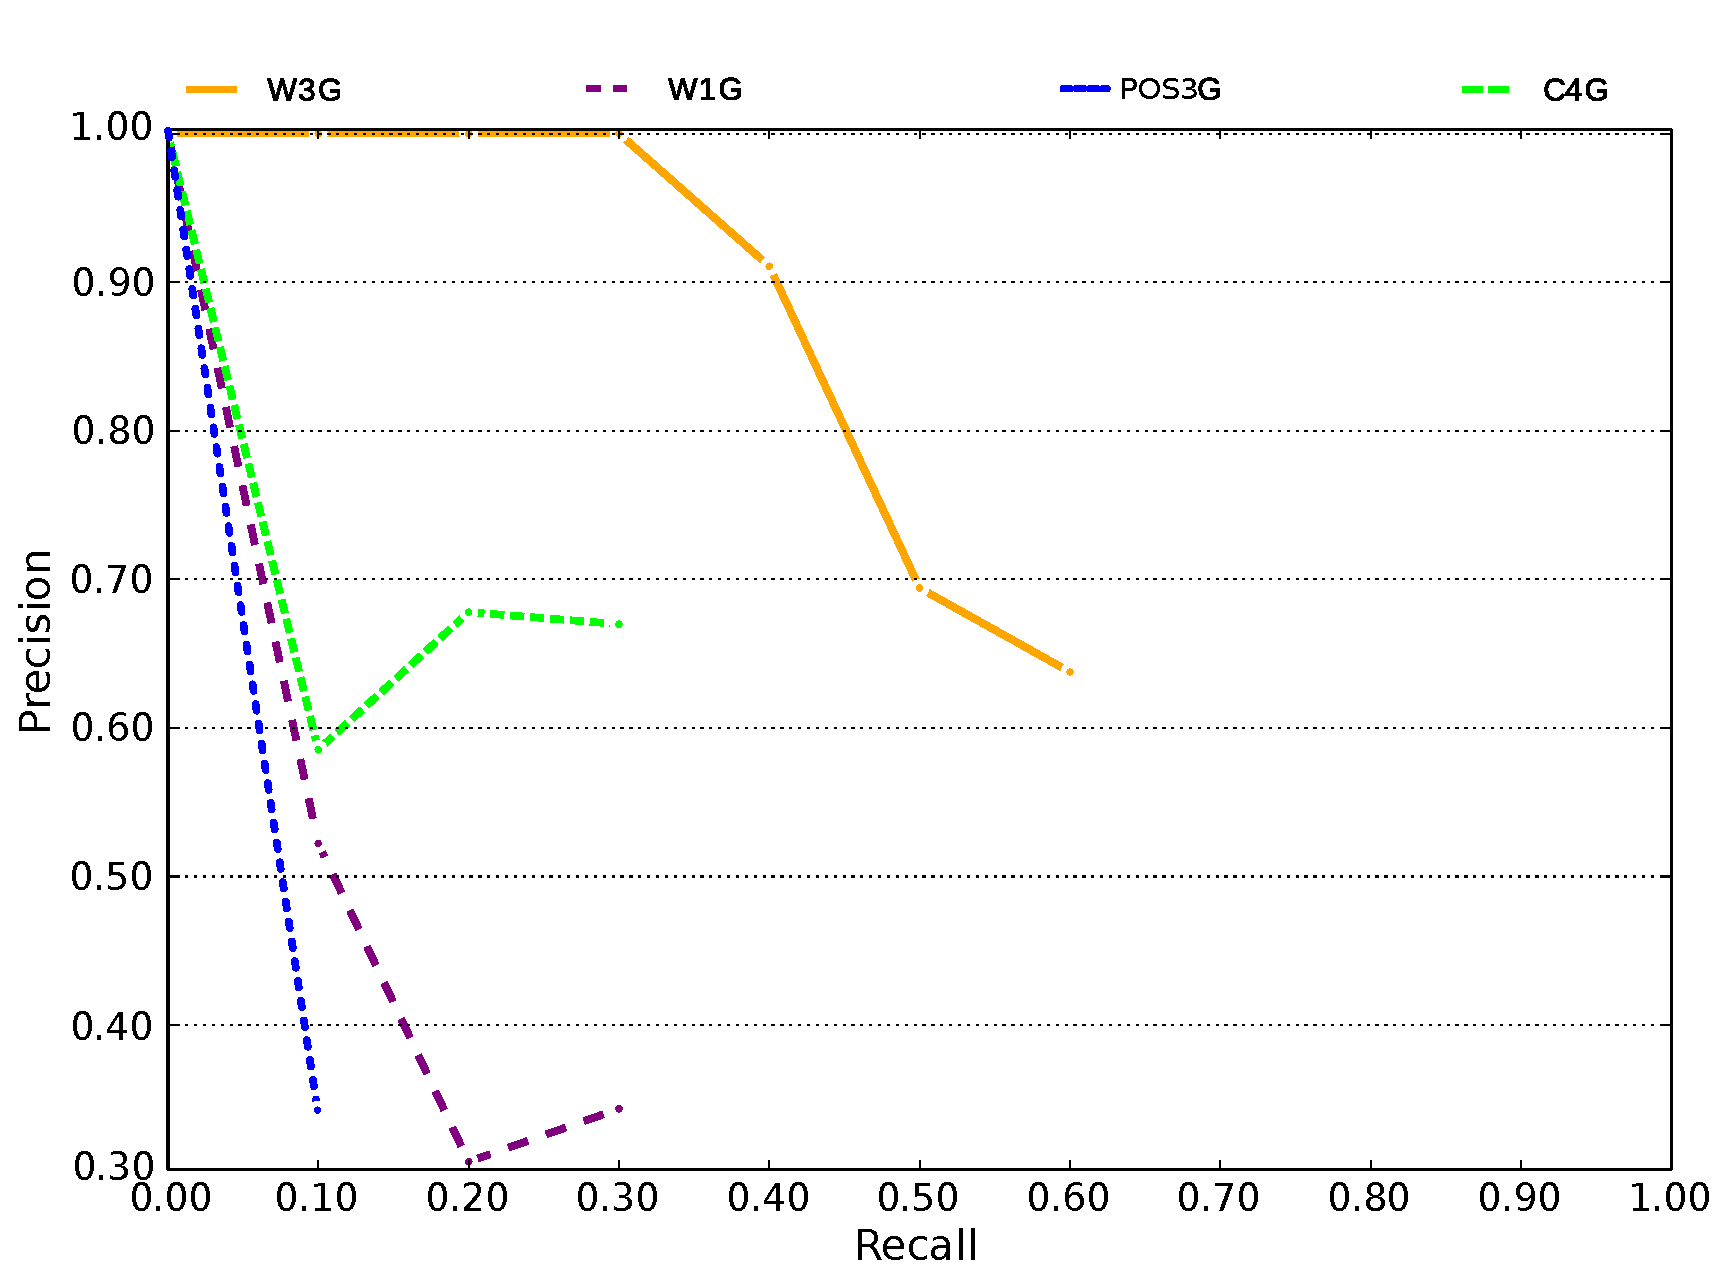
\includegraphics[scale=0.38]{diagrams/OCSME_Best_per_DocRep.eps}
	\caption{Precision-Recall Curves of OCSVM models on SANTINIS corpus using W1G, W3G, and C4G features.}
	\label{fig:MacroPRC_OCSVME_W3G_W1G_C4G_OPTIMAL_SANTINIS}
	\end{center}
\end{figure}

\begin{figure}[H]
\begin{center}
    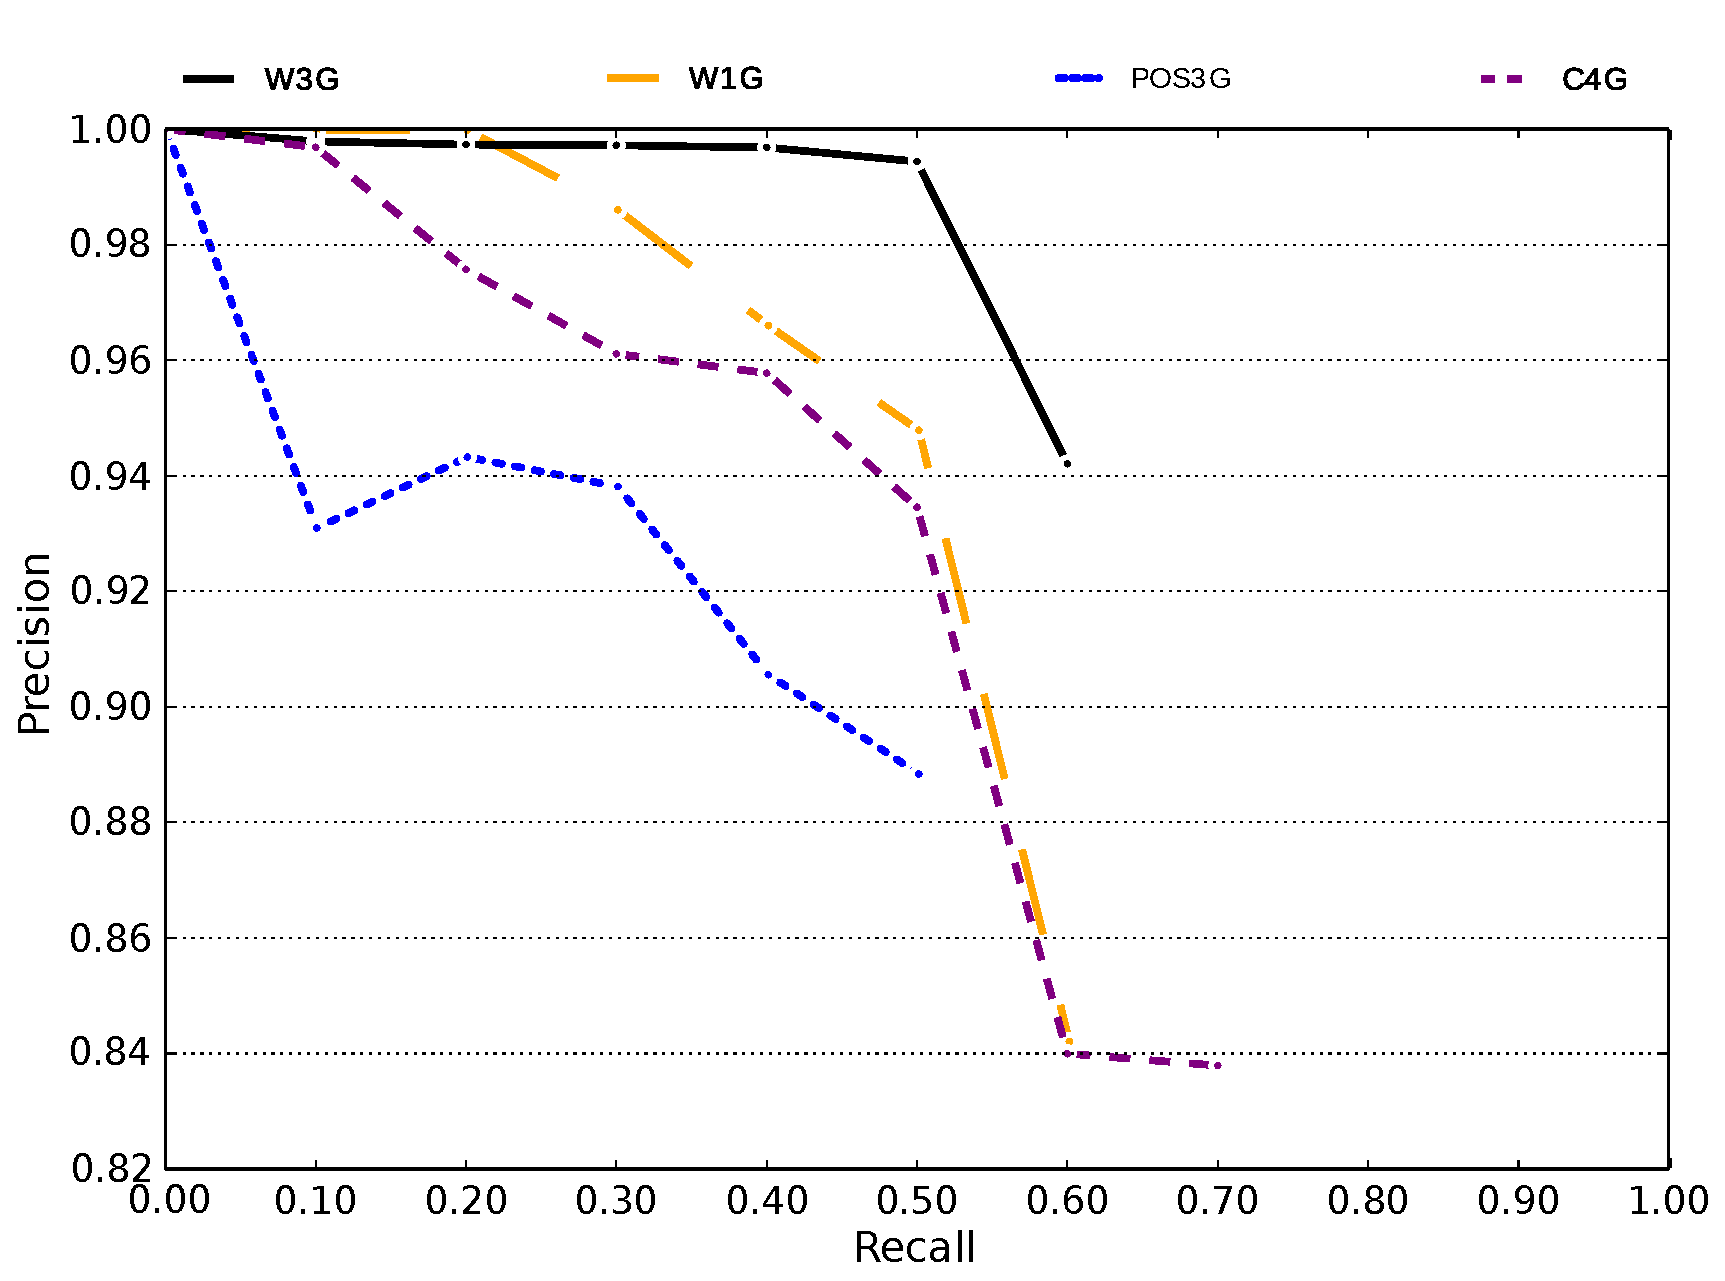
\includegraphics[scale=0.38]{diagrams/RFSE_Best_per_DocRep.eps}
	\caption{Precision-Recall Curves of RFSE models on SANTINIS corpus using W1G, W3G, and C4G features.}
	\label{fig:MacroPRC_RFSE_W3G_W1G_C4G_OPTIMAL_SANTINIS}
	\end{center}
\end{figure}

We further explore the performance of the open-set WGI methods by selecting parameter settings with different optimization criteria. Tables \ref{tbl:OCSVME_SANTINIS} and \ref{tbl:RFSE_SANTINIS} show the combination of parameters that optimize performance of OCSVM and RFSE based on AUC, $F_{1}$ and $F_{0.5}$. Moreover, in the tables we show the values of all three performance measures where one of them is maximized. It is clear that the performance in all cases is maximized when W3G document representation is used. In previous studies based on a closed-set framework, C4G was the document type of features to maximize performance \citep{Sharroff2010}. This indicates that contextual and content information is important for this corpus \citep{Asheghi2015}.

In addition, in almost all cases, RFSE models are far more effective than OCSVM. Another important conclusion is that the optimization criterion plays a crucial role for the properties of the model especially for RFSE. When AUC is maximized, recall is favoured. On the other hand, while $F_{1}$ is maximized, precision is substantially increased. Fig.  \ref{fig:MacroPRC_RFSE_OCSVME_SANTINIS} shows the performance of OCSVM and RFSE models when AUC and $F_{1}$ criteria are used to select parameter settings. As can be seen, the RFSE model based on $F_{1}$ maximization avoids to make wrong decisions and leaves a large number of web pages unclassified. On the other hand, the model optimized by AUC prefers to make a lot of errors in order to recognize more web pages of known genres. OCSVM models seem not significantly affected. Note that choosing between WGI models that prefers precision over recall and vice versa is an application-specific task.

\begin{figure}[H]
\begin{center}
    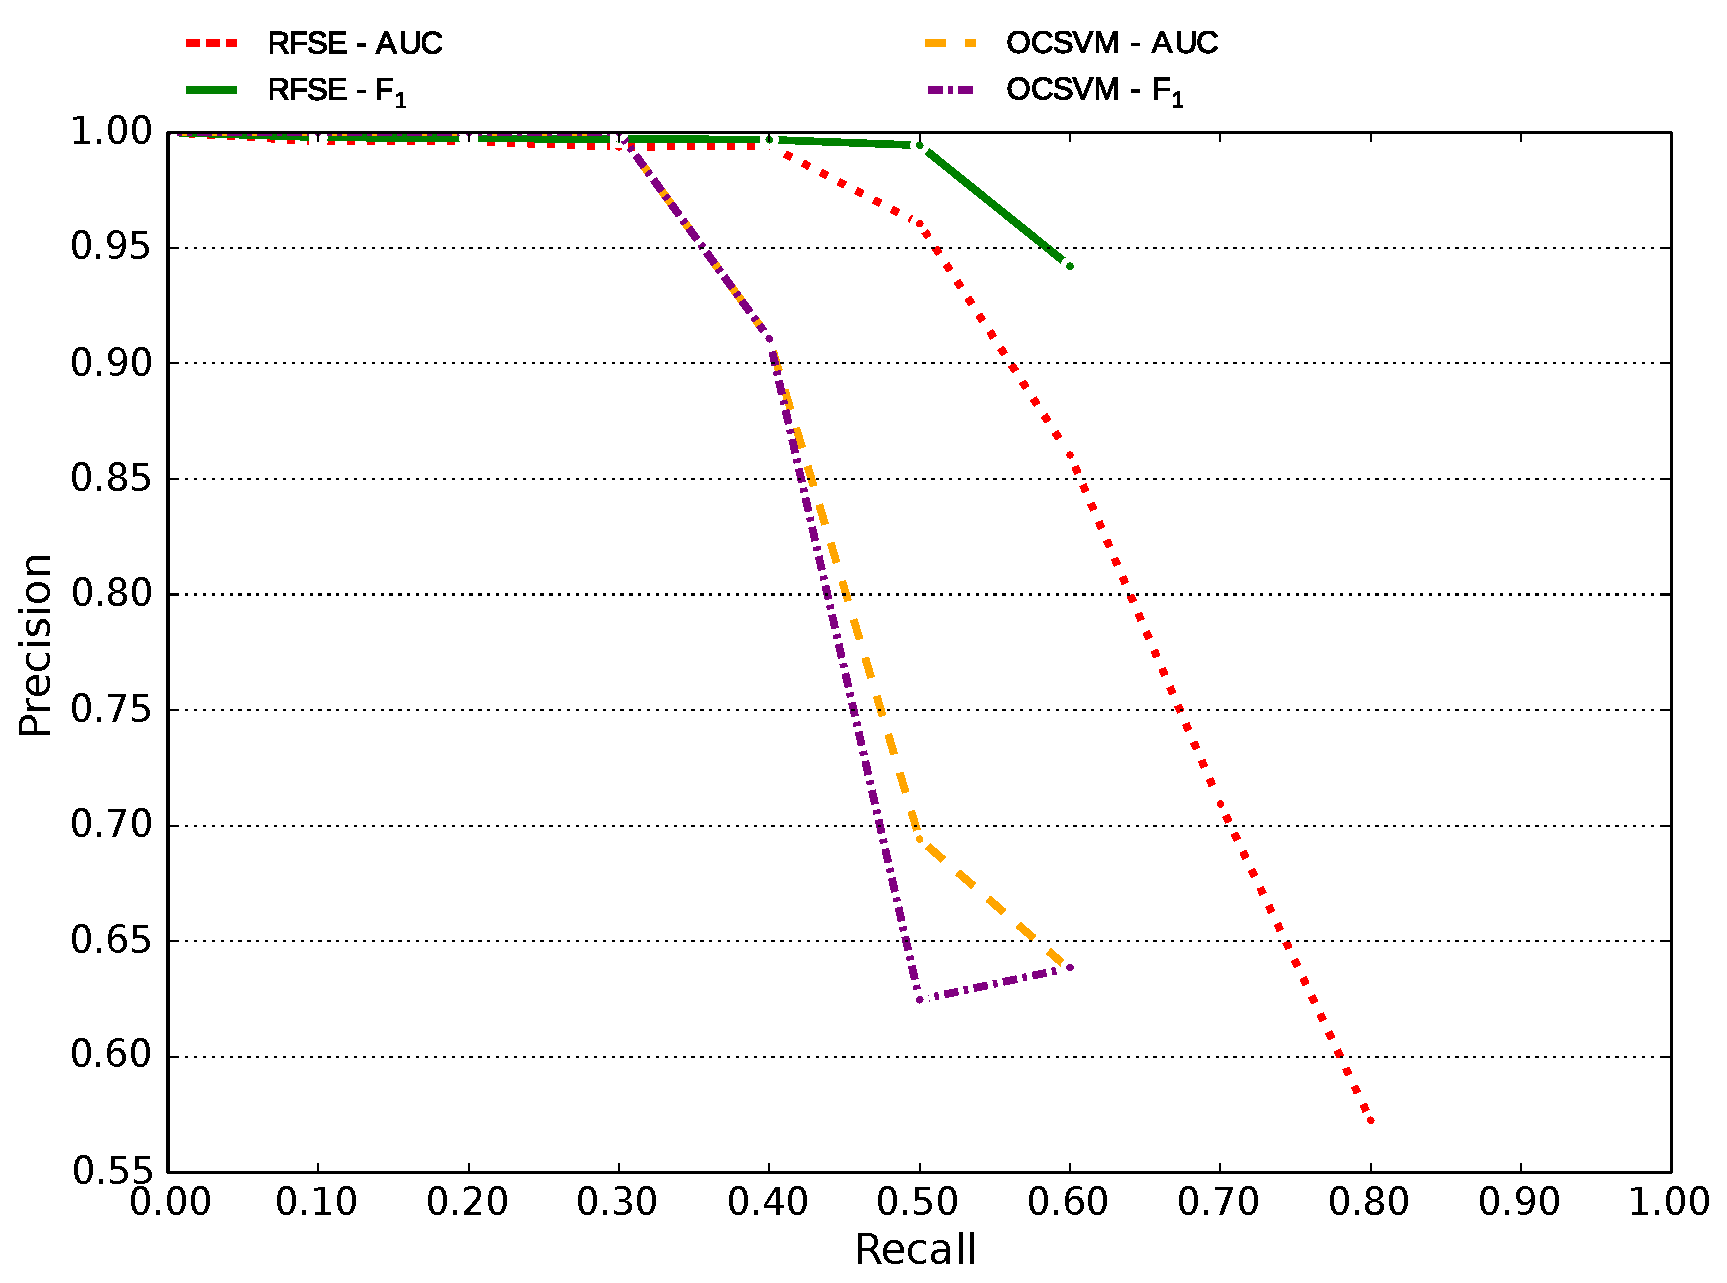
\includegraphics[scale=0.38]{diagrams/MacroPRC11AVG_RFSE_OCSVME_SANTINIS_2.eps}
	\caption{Precision-Recall Curves of OCSVM and RFSE models on SANTINIS corpus optimized either by AUC or $F_{1}$.}
	\label{fig:MacroPRC_RFSE_OCSVME_SANTINIS}
	\end{center}
\end{figure}

% 7Genres
%
\begin{table}[H]
\centering

\pgfplotstableset{
    create on use/Criterion/.style={ create col/set list={AUC, $F_{1}$, $F_{0.5}$} },
	columns/DocRep/.style={string type},
	create on use/DocRep/.style={ create col/set list={W3G, W3G, W3G} },
	columns/DocRep/.style={string type}
}

\pgfplotstabletypeset[
		fixed,
		precision=3,
		col sep=comma,
		every head row/.style={
			before row = \toprule,
			after row=\midrule,
		},
		every last row/.style={after row=\bottomrule \\},
		columns={Criterion, DocRep, 0, 1, 2, 3, 4, 5, 6, 7},
		columns/Criterion/.style ={string type,column type=c, column name=Optim.},
        columns/DocRep/.style ={string type,column type=c, column name=Features},
		columns/0/.style ={column type=c, column name=Voc.},
		columns/1/.style ={column type=c, column name=\textit{f}},
		columns/2/.style ={column type=c, column name=$\nu$},
		columns/3/.style ={column type=c, column name=Prec.},
		columns/4/.style ={column type=c, column name=Rec.},
		columns/5/.style ={column type=c, column name=AUC},
        columns/6/.style ={column type=c, column name=$F_{0.5}$},
        columns/7/.style ={column type=c, column name=$F_{1}$},
		]{tables_data/AUC_FStatistics_tables/OCSVME_SANTINIS_Best.csv}
\caption{Best performing models for OCSVM on SANTINIS corpus.}
\label{tbl:OCSVME_SANTINIS}
\end{table}

\begin{table}[H]
\centering

\pgfplotstableset{
    create on use/Criterion/.style={ create col/set list={AUC,$F_{1}$,$F_{0.5}$} },
    columns/DocRep/.style={string type},
	create on use/DocRep/.style={ create col/set list={W3G,W3G,W3G} },
	columns/DocRep/.style={string type},
    create on use/SimMeas/.style={ create col/set list={Combo,MinMax,MinMax} },
	columns/SimMeas/.style={string type}
}

\pgfplotstabletypeset[
		fixed,
		precision=3,
		col sep=comma,
		every head row/.style={
			before row = \toprule,
			after row=\midrule,
		},
		every last row/.style={after row=\bottomrule \\},
		columns={Criterion, DocRep, SimMeas, 0, 1, 2, 3, 4, 5, 6, 7, 8},
        columns/Criterion/.style ={string type,column type=c, column name=Optim.},
		columns/DocRep/.style ={string type,column type=c, column name=Features},
        columns/SimMeas/.style ={string type,column type=c, column name=Similarity},
		columns/0/.style ={column type=c, column name=Voc.},
		columns/1/.style ={column type=c, column name=\textit{f}},
		columns/2/.style ={column type=c, column name=$\sigma$},
        columns/3/.style ={column type=c, column name=\textit{I}},
		columns/4/.style ={column type=c, column name=Prec.},
		columns/5/.style ={column type=c, column name=Rec.},
		columns/6/.style ={column type=c, column name=AUC},
        columns/7/.style ={column type=c, column name=$F_{0.5}$},
        columns/8/.style ={column type=c, column name=$F_{1}$},
		]{tables_data/AUC_FStatistics_tables/RFSE_SANTINIS_Best.csv}
\caption{Best performing models for RFSE on SANTINIS corpus.}
\label{tbl:RFSE_SANTINIS}
\end{table}


\subsection{WGI with Structured Noise}
\label{sec:openness_evaluation}

In this section we describe experiments using a corpus with structured noise, i.e., when the true genre of pages not included in the training genre palette is available. In more detail, we use the KI-04 corpus and adopt the openness measure varying the number of training classes from 7 to 1 while keeping the number of testing classes always the same, at maximum 8. As a result, the openness measure varies from 0.065 to 0.646, one extreme refers to the case where only one genre class is unknown while in the other extreme only one genre class is known. For each openness level, we randomly select the known classes and repeat the experiment 8 times, each time performing 10-fold cross-validation. Moreover, to avoid any biased selection of parameter values, we use the parameter settings found to be optimal for the SANTINIS corpus in section \ref{sec:WGI_noise}.

Figures \ref{fig:OCSVME_openness_test} and \ref{fig:RFSE_openness_test} show the performance ($F_{1}$) of OCSVE and RFSE models using different text representation features for varying openness levels. Standard error bars are also depicted to show the variance of performance for each model. Surprisingly, the performance of OCSVM seems to improve by increasing openness and this pattern is consistent in all three feature types while C4G seem to be the most effective type. On the other hand, RFSE models based on C4G and W1G gradually get worse while openness increasing while W3G models seems to be relatively stable.

\begin{figure}[H]
\begin{center}
    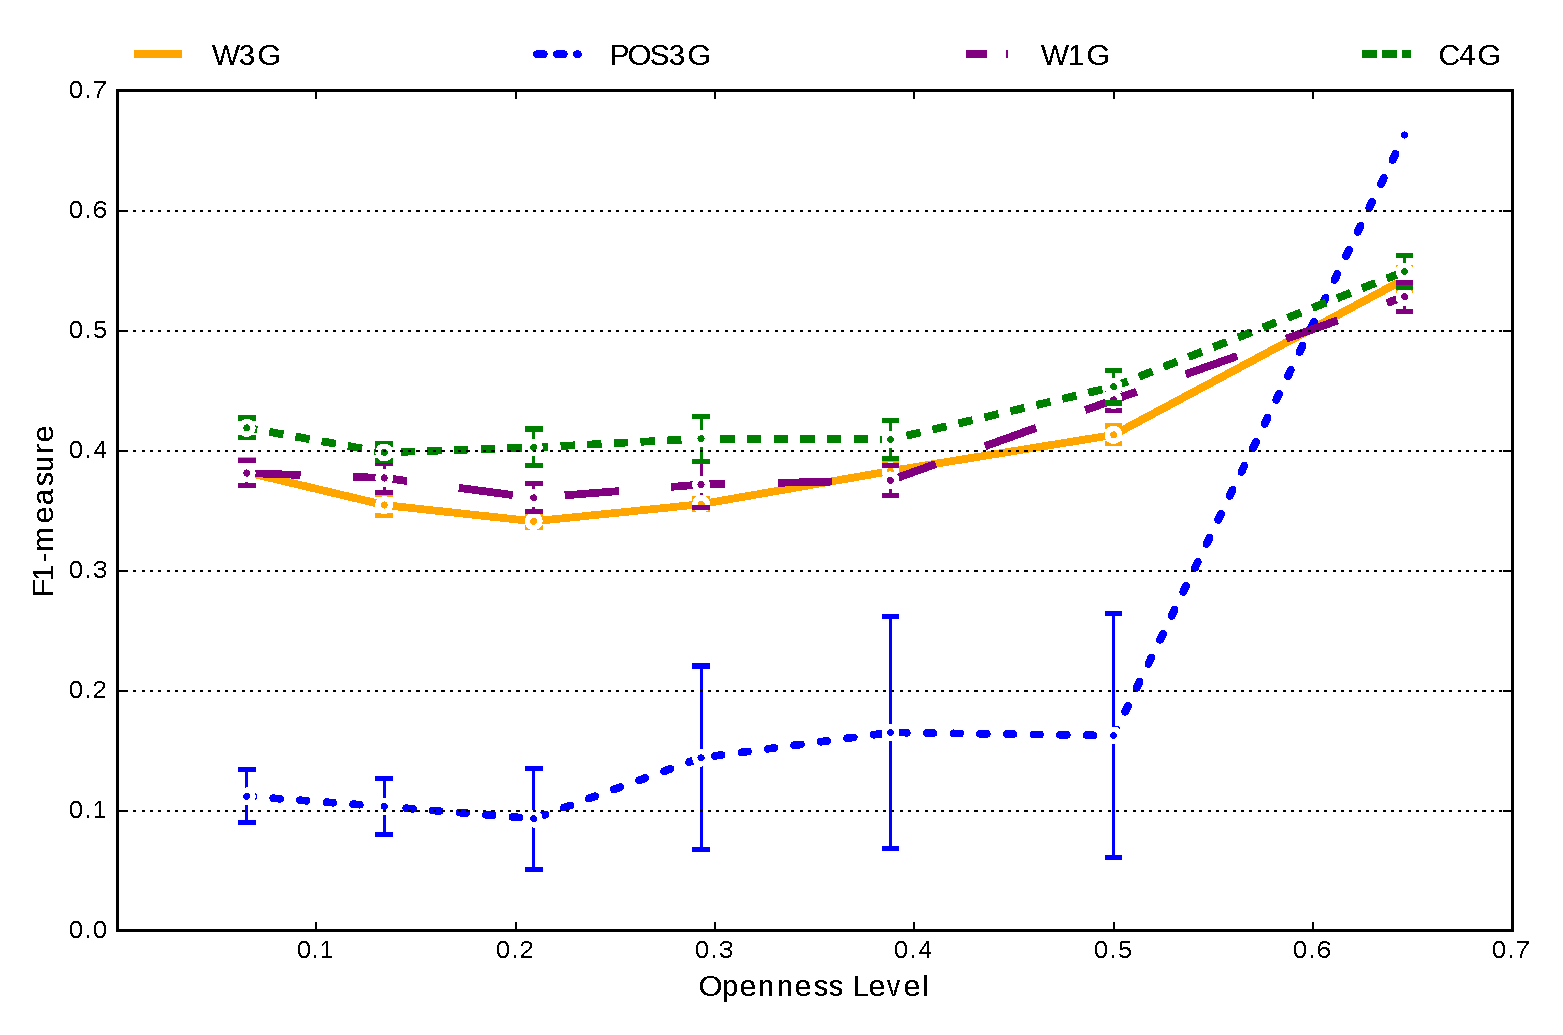
\includegraphics[scale=0.38]{diagrams/OCSVME_openness_test_graph.eps}
	\caption{OCSVM performance in varying openness level.}
	\label{fig:OCSVME_openness_test}
\end{center}
\end{figure}

\begin{figure}[H]
\begin{center}
    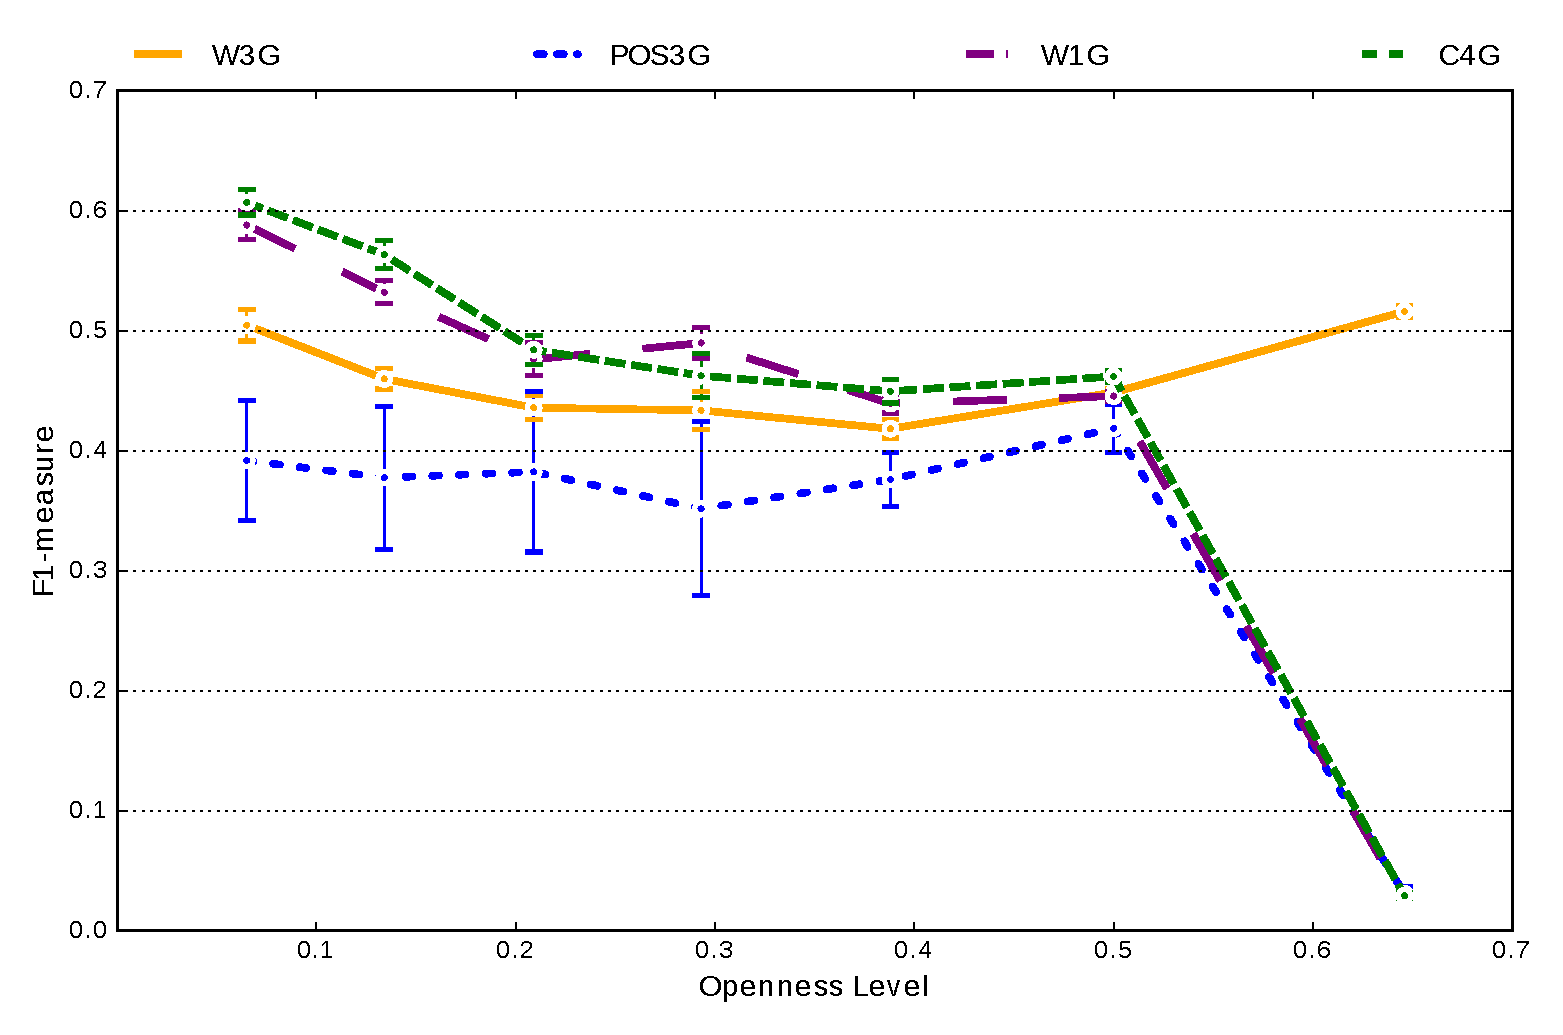
\includegraphics[scale=0.38]{diagrams/RFSE_MIX_openness_test_graph.eps}
	\caption{RFSE performance in varying openness level.}
	\label{fig:RFSE_openness_test}
\end{center}
\end{figure}
%
%
% APPEND by Dp - Start

As it was highlighted in the previous section, according to the properties of the application in which WGI is involved, precision may be more important than recall or vice-versa. In figure \ref{fig:RFSE_precision_focus_openness_test} the macro-precision of RFSE is depicted for W3G, W1G and C4G features. MinMax similarity is used since it increases significantly the performance of RFSE in respect with precision. As concerns text representation, W1G is the best choice when precision is at more importance than recall. On the other hand, W3G features seem to be more stable because the standard error is lower than that of the other features and also the W3G model is not affected too much when openness surpasses $0.5$ (actually it improves).

\begin{figure}[H]
\begin{center}
    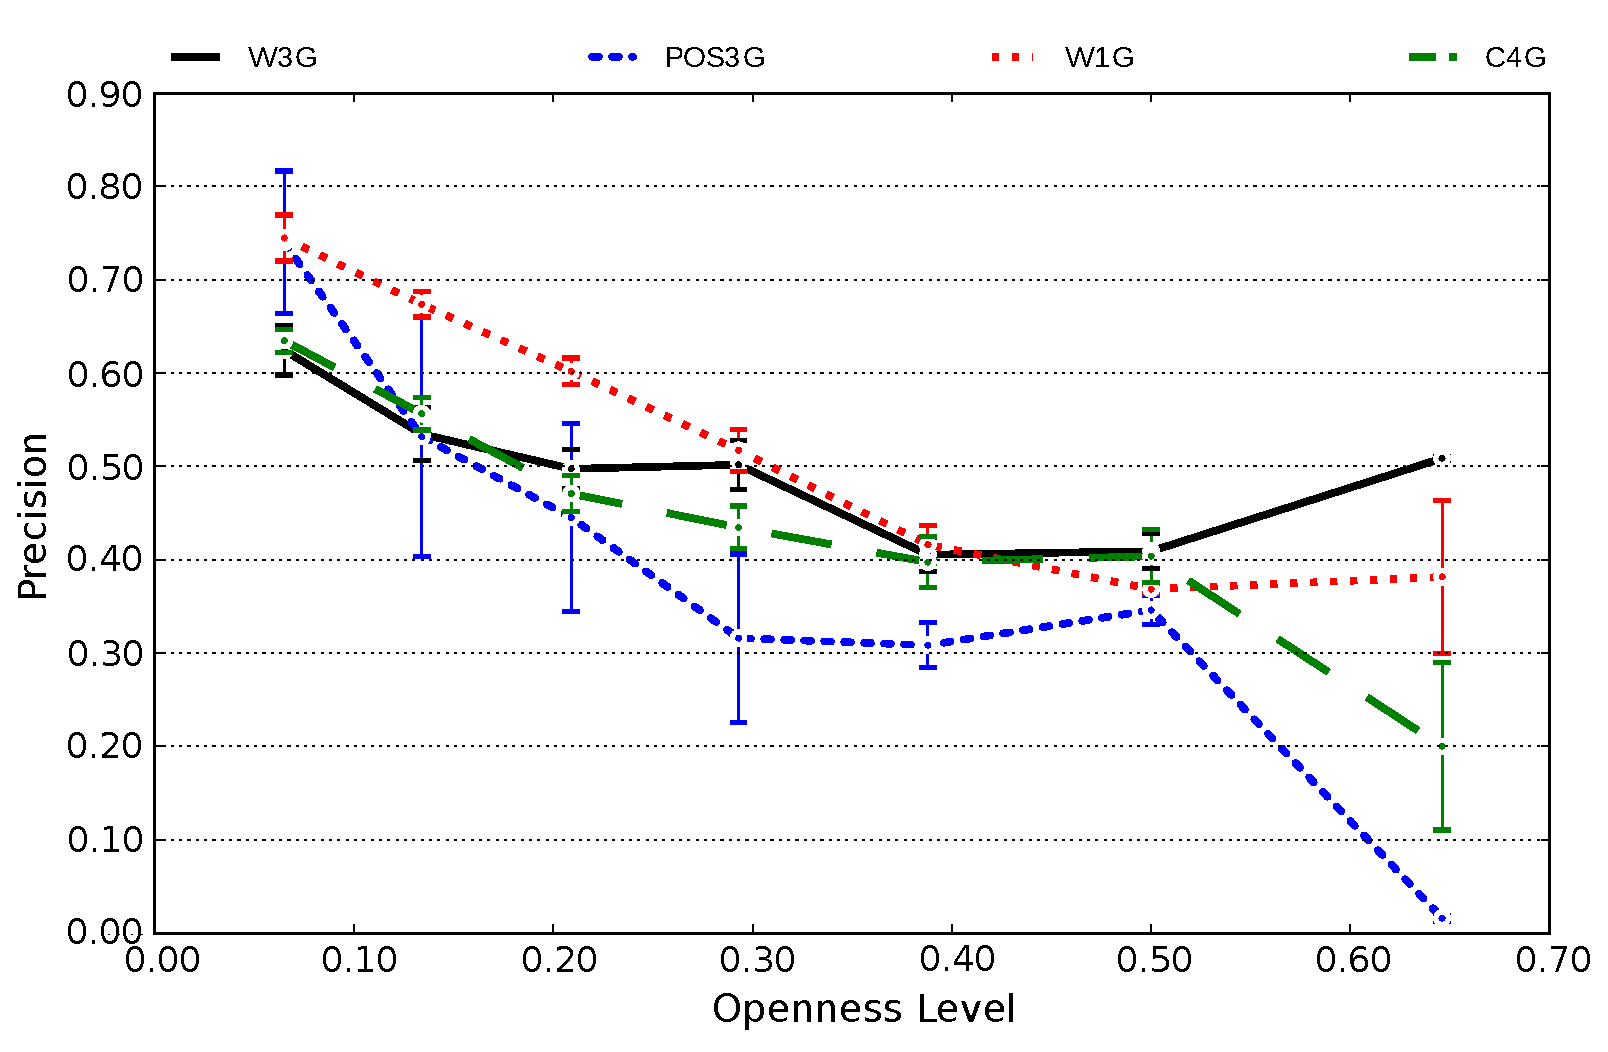
\includegraphics[scale=0.38]{diagrams/RFSE_Precision_Focus_openness_test_graph.eps}
	\caption{RFSE precision in varying openness level.}
	\label{fig:RFSE_precision_focus_openness_test}
\end{center}
\end{figure}

In the case of C4G and W1G where the openness level is $0.646$ the standard error in both case is very hight. Since, we observe this problem only in the case where the problems has been reduced to binary, we are interested to see whether it is caused by choice of the document representation or by the choice of the similarity measure.

%In figures \ref{fig:RFSE_MIXvsMinMax_W3GvsC4G_openness_test} the $F_{1}$ measure performance in %the openness test of the RFSE is depicted. In all three cases we see the only with MinMax %similarity the standard error is significantly high especially in the case of $0.646$ openness %level.

Despite OCSVM's improvement when structured noise is used, it can only be competitive to RFSE on a high openness level, where all genre labels but one are considered unknown. This can be better viewed in figure \ref{fig:RFSE_vs_OCSVME_W1G_openness_test} where OCSVM is compared with RFSE models based on MinMax and Combo similarity measures for a varying openness level. These curves correspond to W1G features, so they are not the optimal models. However, they provide a fair comparison between examined methods. As standard error bars indicate, the performance of RFSE models with respect to the $F_{1}$ measure is significantly better than that of OCSVM while openness is less than $0.5$. Beyond that level, OCSVM is significantly better than RFSE models. Note also Combo measure helps RFSE in while openness is relatively low and MinMax seems to be a better choice when openness increases.

\begin{figure}[H]
\begin{center}
    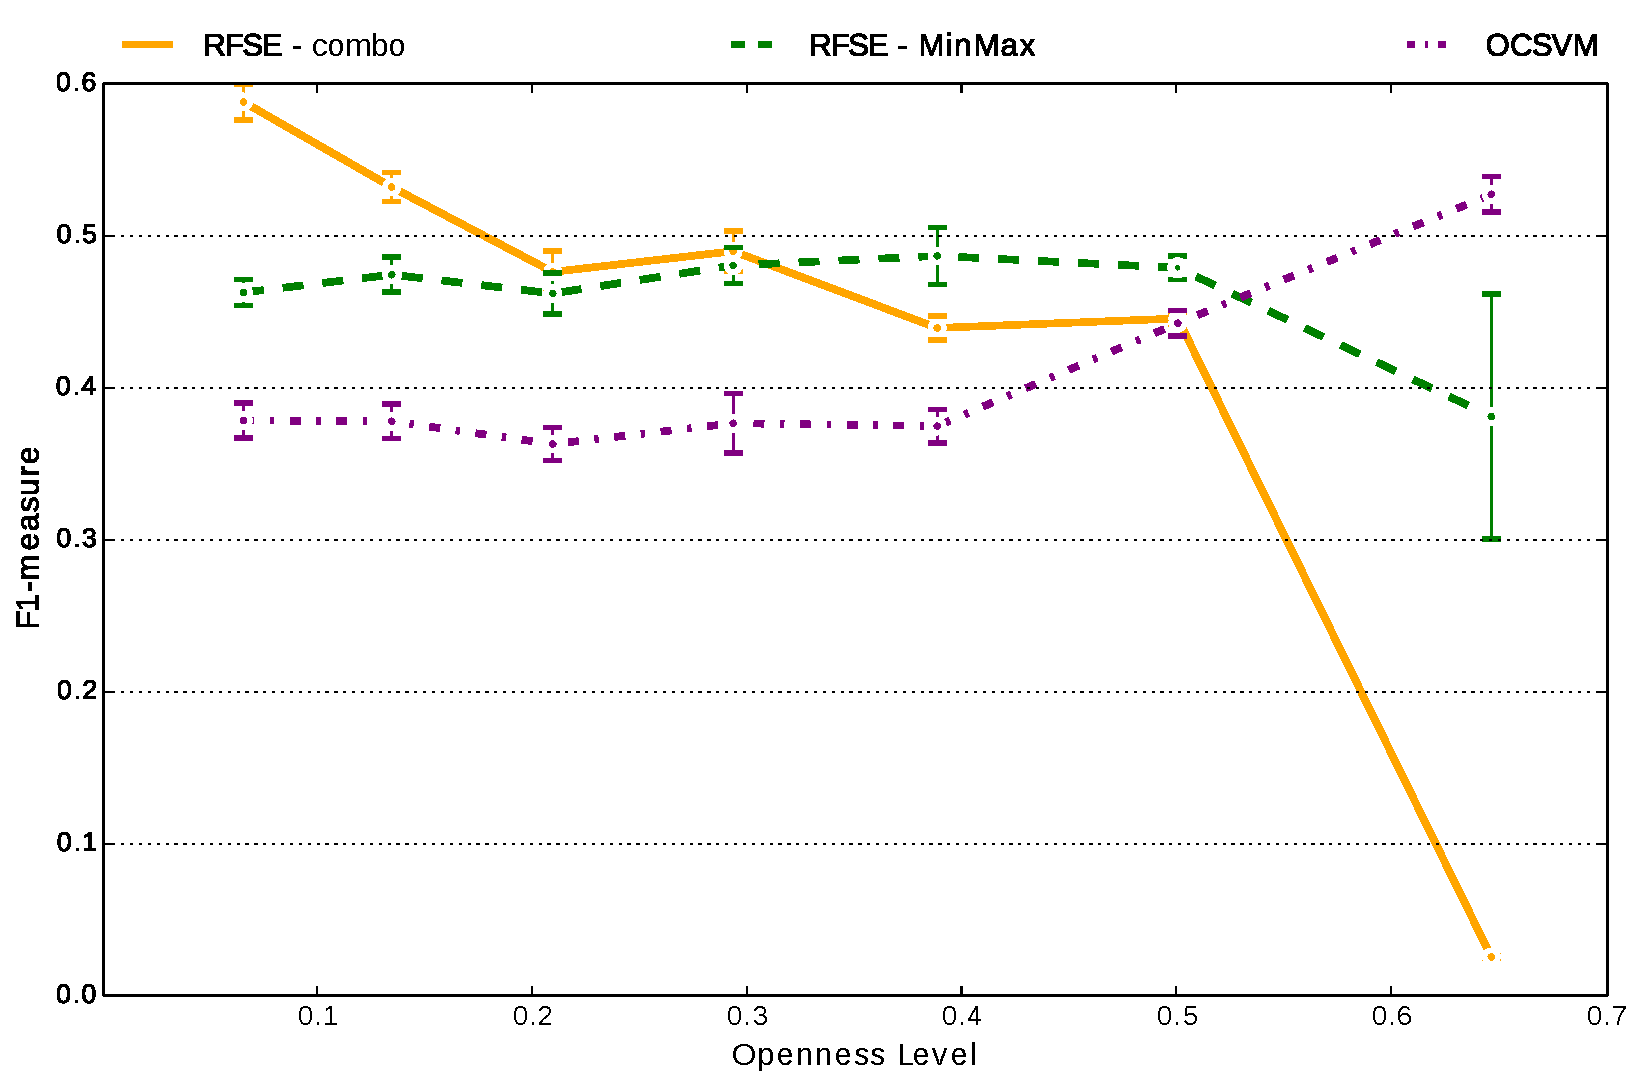
\includegraphics[scale=0.38]{diagrams/RFSE_vs_OCSVME_W1G.eps}
	\caption{Comparison of OCSVM and RFSE models based on W1G features in varying Openness levels.}
	\label{fig:RFSE_vs_OCSVME_W1G_openness_test}
\end{center}
\end{figure}

\section{Conclusions}\label{sec:conclusions}

In this paper we presented an experimental study on WGI focusing on open-set evaluation for this task. In contrast to vast majority of previous work in this area, we adopt the open-set scenario that is more realistic for WGI since it is not feasible to construct a genre palette with all available genres and appropriate samples for each one of them. Moreover, we examined two open-set classification methods and several feature types and similarity measures. To the best of our knowledge, this is the first time the performance of WGI models is evaluated using performance measures and tests specifically designed for open-set classification tasks.

The presented evaluation of open-set WGI covers two basic scenarios. The first is when noise is unstructured, i.e., information about the true genre of pages not belonging to the known genre palette is not available. The second scenario applies when noise is structured, i.e., we actually know the true genre of pages not included in the training classes. For both cases, we propose appropriate evaluation methodologies and present comparative results for the tested models.

In almost all examined cases, RFSE models outperformed the corresponding OCSVM models. This verifies previous work findings about the appropriateness of RFSE for WGI \citep{pritsos2013open}. RFSE is able to provide effective models and additionally it is possible to manage preference on recall or precision, an application-dependent choice, by focusing on optimizing AUC or $F_1$ respectively. On the other hand, OCSVM proved to be the best-performing method in extreme cases when openness is high. Actually, the restrictions of the available corpora did not allow us to examine cases where openness approaches $1.0$. However, it seems that when openness is more than $0.5$ OCSVM outperforms RFSE.

As concerns the feature types, in most of the cases W3G and C4G provided the best results. However, the selection of text representation features is a crucial choice that affects performance and it seems to be corpus-dependent. Another crucial parameter of RFSE is the similarity measure. Among the examined measures, MinMax and its combination with cosine similarity provide the most robust results. The choice of similarity measure correlates with feature types. It seems that the combo measure is more effective than MinMax in low openness conditions.

To enhance the evaluation of WGI models in open-set conditions, we need larger corpora including multiple genre labels. New enhanced open-set WGI methods are needed and they should be evaluated using the proposed paradigm. Otherwise, using an evaluation paradigm more appropriate for closed-set tasks, the performance may be over-estimated.
\include{Chapters/Document_representation}

%!TeX spellcheck = en-US
%\chapter{Word Embedding and Distributional Features of the web-pages and texts}
\chapter{The Usefulness of Distributed Representation in WGI}

\label{chap:word_embeddings}


%----------------------------------------------------------------------------------------

% Define some commands to keep the formatting separated from the content
\newcommand{\keyword}[1]{\textbf{#1}}
\newcommand{\tabhead}[1]{\textbf{#1}}
\newcommand{\code}[1]{\texttt{#1}}
\newcommand{\file}[1]{\texttt{\bfseries#1}}
\newcommand{\option}[1]{\texttt{\itshape#1}}

%----------------------------------------------------------------------------------------

\section{Introduction}\label{chap:word_embeddings:sec:intro}
 
The most traditional text representation scheme in text mining tasks is the Bag of Words (BOW) model which is based on individual tokens as features. It is a simplistic approach to quantify information documents assuming independence of the occurrence of individual tokens in documents. The result is a document vector of high dimensionality (i.e., in the order of thousands of features) and sparseness (i.e., only a few non-zero values per document). The BOW model is not able to capture information about the grammar of documents and completely ignores word order. In addition, it is confused by synonym terms since it assumes they are independent. Nevertheless, it provides an easy and quite competitive approach to represent documents (the W1G scheme used in Chapter \ref{chap:noise} is actually based on BOW).

A more elaborate text representation scheme is to consider n-gram of words. This would capture information about word sequences, like phrases. This can improve the ablity of the model to represent syntactic information since the context of words is partially taken into account (e.g., the W3G model used in Chapter \ref{chap:noise}). Nevertheless, the dimensionality of representation is considerably increased when the order of the model ($n$) is high. In addition, the sparseness of the vectors is increased. It is also possible to apply the n-gram approach on the character level or on POS-tag level, as shown in the experiments of Chapter \ref{chap:noise} (i.e., C4G, POS3G). The main assumption that each feature (n-gram) is independent of the other features is still valid in such models.

An alternative approach is to use \textit{distributed representations} that attempt to introduce some kind of dependence of each word (or n-gram) on the other words (or n-grams). For example, the words usually encountered in the context of a specific word are more dependent on that word. In addition, different words found in similar context get a higher share of dependence. Distributed representations can be obtained by applying language modeling methods. Especially, the use of neural network language models and the popular word and document \textit{embeddings} introduced in \parentcite{mikolov2013distributed}. 

One main advantage of distributed representations is that they provide compact (i.e., low-dimensional) and dense vectors to quantify syntactic and semantic information in documents. In comparison to regular BOW or n-gram models, distributed features are much less redundant and irrelevant since each such feature captures a combination of information that cannot be specifically determined. Therefore, it seems that open-set WGI methods that are not able to easily handle high-dimensional, sparse vectors with many irrelevant and redundant features would be highly improved by using distributed representations. As already explained in Chapter \ref{chap:openset}, NNDR is an algorithm that, in theory, is vulnerable when it is not combined with appropriate feature sets. The main goal of this Chapter is to examine how the performance of NNDR in WGI tasks can be improved when distributed features are used. 

The rest of this chapter is organized as follows. First, the main ideas of distributed representation are presented. Then, the specific distributed features used in this thesis are described. Next, we compare the performance of NNDR using traditional sparse representation schemes with the case dense vectors are used. We also compare these versions of NNDR with OCSVM and RFSE methods and discuss the main conclusions of this study.

\section{Obtaining Distributed Representations}

%The SLM model is defined as the \textit{joint conditional probability distribution} of the next word given the probabilities of previous ones as shown in equation \ref{chap:word_embeddings:eq:slm}

%\begin{equation} \label{chap:word_embeddings:eq:slm}
%	P(w = i) = \prod_{i=1}^{|V|} P(w_{i}|w_{i-k}, ... , w_{i+k})
%\end{equation}
%\noindent
%where $w_{i}$ is the i-th word, and $k$ is for the number of words before or/and and after, writing sub-sequence $w_{i} = (w_{i-k}, w_{i-1}, ... ,w_{i+1}, w_{i+k})$. Note that this model returns a singleton value for a word on the condition of previews or/and next word. This model also can be expanded to have few more words in the conditional probability, usually from 2 up to 4. 

%With this model it can be captured the semantic proximity but it will return zero in the case a sequence have never been met before in the samples. A solution to this problem is the interpolation or smoothness factor that can be applied such as in the \textit{back-off}  model (Katz, 1980 see in bengio2003neural). 

%The model of equation \ref{chap:word_embeddings:eq:slm} can capture the joint probability of word-sequences in terms of feature vectors, however, it cannot capture the correlation of the words in terms of semantics. Models like LSI or LDA are methodologies also been tested in IR and NLP for capturing the semantics in the context of the n-gram based SLM. 

One way to obtain a low-dimensional and dense representation of documents is the use of topic modeling. Topic modeling methods attempt to group terms according to their co-occurrence in documents. They provide a new feature space (composed by latent topics) of pre-defined dimensionality. One popular topic modeling approach is \textit{Latent Semantic Analysis}, a linear algebraic method that transforms a high-dimensional and sparse representation to a low-dimensional and dense one applying \textit{singular value decomposition} \parentcite{Kontostathis:2006}. Another popular approach is \textit{Latent Dirichlet Allocation}, a generative probabilistic where each documents is represented as a mixture over a set of latent topics. Each topic is in turn defined as a distribution over words \parentcite{Blei:2003}.

Another main direction that gained huge popularity during the last years is the use of neural probabilistic language models \parencite{bengio2003neural}. We first describe how words can be represented in a coninuous space and then we focus on documents.

\subsection{Word Embeddings}

The main idea is that words can be represented by real vectors (word embeddings) that are learned by a neural network \parentcite{mikolov2013efficient}. This is unsupervised learning since documents need not be labeled. The neural network is trained to recognize words that occur in similar context. Then, each word is represented in continuous vector space and similar words tend to cluster in the same area. In addition, the distance between related words is affected by semantic similarity (e.g., the difference between terms "king" and "man" is close to the difference between "queen" and "woman") \parentcite{mikolov2013efficient}. 

In practice the distributed features is the mapping of the vocabulary words $V = \{w_{i}, i \in [1, |V|] \}$ to a real vector $\vec{t}_i \in \mathbb{R}^{m}$.

%Then the semantic distance can be approximated by a NNet algorithm given the distribution of the words. The words are initially are having a vector 1-of-V representation, a.k.a. \textit{One-hot representation}. Then the probability of the a word $w_{i}$ in equation \ref{chap:word_embeddings:eq:slm} can be replaced by the real continues vector $t{i}$ and the conditional probability $P(.|.)$ to be approximated my a NNet function $\hat{p}(.)$. The $\hat{}$ (hat) is for symbolizing a special condition where the probability is approximated given a sequence with a specific order, say preceding words or succeeding words or both. 

%Now the DF neural model can be calculated with several architectures where the $\vec{t}$ and the $\hat{p}$ continues distribution can feed separate layers of joint layers, and also the learning strategy can have variant implementations such as Continues Bag-of-Words, Skip-grams etc. The strategy of learning and the NNet architecture are very close related and the results are \textit{continues probability functions with substantially different meaning}, where they can either encode word similarities, word semantics or even paragraph and documents encoding and similarities. 

One basic architecture is the Continuous Bag-of-Words (CBOW) model which attempts to predict a word given its context. This is a \textit{Feedforward Neural Network} with an input layer, a projection layer, and an output layer as shown in figure \ref{chap:word_embeddingss:fig:CBOW_diagram}. The input layer is composed by the context of a word (i.e., the few words immediately to its right and left). Every word in the vocabulary is assigned to a \textit{one-hot} vector $\hat{t}_{i}$ (i.e., a vector of size $|V|$ with all but one values equal to zero). The sequence of context word vectors are added and form the input vector $\hat{t}_{i*}$. Since the order of words is not important in this setting, the model bears similarities to Bag-of-Words \parencite{mitra2018introduction}.

%W_{in}$ is the weight matrix of the projection layer with regularization parameters $\theta$. Now the $\vec{t}$ is the input to a hidden layer $\vec{h}=\vec{t}H$, which is usually the \textit{hyperbolic tangent hidden layer}, where $H$ is the weights of the hidden layer. Then, the output $\hat{p}=\vec{h}W_{out}$ is the last layer of the NNet.

\begin{figure}[t]
	\begin{center}
    	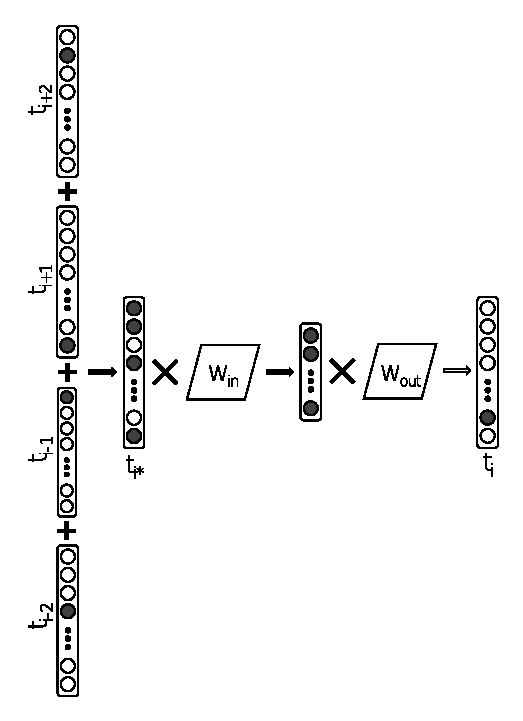
\includegraphics[scale=0.99]{Figures/CBOW_diagram.eps}
		\caption{Diagram for C-BOW and General NLM architecture. Depending whether the $t_{i*}$ is part of the projection and the hidden layer or the layers are different. In practice the weighting matrices are either shared or diff rent between the word projection and the hidden layer or it is the same matrix, which is equivalent to the words been projected to the same position as their vectors are averaged and not concatenated.}
		\label{chap:word_embeddingss:fig:CBOW_diagram}
	\end{center}
\end{figure}

%The generic architecture of the final output of the NLM described above is the equation \ref{chap:word_embeddingss:nlm_generic}. Note that the output vector $\vec{y}$ has size $|V|$ due to the input $\hat{w}$ and is the inference model of a \textit{continues distribution} of both the proximity of the words in the sentences (captured by the hidden layer) and the distribution over the vocabulary, which is the continues similarity of the words in this vocabulary. The output layer then is as described in equation \ref{chap:word_embeddings:eq:NLM}

%\begin{equation} \label{chap:word_embeddings:eq:NLM}
%	\vec{y} = \vec{t} + W_{out}(\vec{t}H + b_{h}) + b_{o}
%\end{equation}

%\noindent
%where $b_{o}$ and $b_{h}$ are the output and hidden layers biases. Usually the Hidden layer typically has a size of 500 to 1000 neurons while the projection layer might be 500 to 2000. Due to the multiple layers and the feeding of both the projection and the hidden to the output layer there is great complexity and the process is very computationally demanding. 

%A more efficient method is suggested in \parencite{mikolov2013efficient} where the non-linear hidden layer is removed and the projection layer is shared to all words, geometrically this is equivalent to the projection of the words to the same position. Then the algorithm is reformed and the $\hat{w}$ vectors are replaced by the $t^{*}$ which is the sum of the \textit{one-hot word vectors} \parencite{mitra2018introduction}. 

%Now the equation \ref{chap:word_embeddings:eq:NLM} is becoming \ref{chap:word_embeddings:eq:CBOW}. Due to the new form of the NNet where the tangent hidden layer is absent, there is no constraint in the presenting sequence of the words order. Moreover, the succeeding words also can also be taken in to account in a given \textit{window} say for $k_{w}$ number of words around the specific one. 

The weight matrix $W_{in}$ is of size $|V| \times m$ while $W_{out}$ is of size $m \times |V|$, where $m$ is the size of the hidden layer ($m << |V|$) and it also corresponds to the dimensionality of the extracted distributed representation. The size of the output vector is equal to the vocabulary size. 
%
%\begin{equation} \label{chap:word_embeddings:eq:CBOW}
%	\vec{y} = \hat{t}_{i*} \times W_{out} + b_{o}
%\end{equation}

During training, CBOW attempts to learn weight matrices $W_{in}$ and $W_{out}$. The loss function of CBOW is the following conditional log probability: 

\begin{equation} \label{chap:word_embeddings:eq:CBOW_log_likelihood}
	 \mathcal{L}_{CBOW} = -\frac{1}{|S|} \sum_{i=1}^{|S|}{\log{p(t_{i}|t_{i-k}, ... ,t_{i+k})}}
\end{equation}

\noindent
where $k$ is the size of context words, $S$ is the amount of possible context windows. \textit{Stochastic Gradient Decent} and \textit{Backpropagation} are used to train that network. CBOW is actually a encoder-decoder model and applies a \textit{SoftMax} function in its output: 

\begin{equation} \label{chap:word_embeddings:eq:CBOW_softmax}
	p(t_{i}|t_{i-k},...,t_{i+k}) = \frac{e^{y_{t_{i}}}}{\sum^{|V|}_{i}{e^{y_{t_i}}}}
\end{equation}

\nointdent where $y_{t_i}$ is the output vector for term $t_i$.

Another architecture is the \textit{skip-gram} model, that attempts to predict the context of a word. This is depicted in figure \ref{chap:word_embeddingss:fig:skipgram_diagram}. Again, input and output are one-hot vectors while the hidden layer is of dimensionality $m$ ($<<|V|$). The objective is to learn weight matrices $W_{in}$ and $W_{out}$ and the loss function is as follows:

\begin{equation} \label{chap:word_embeddings:eq:skipgram_log_likelihood}
	 \mathcal{L}_{SkipGram} = -\frac{1}{|S|} \sum_{i=1}^{|S|}{ \sum_{-k \leq j \leq +k}{ \log {p(t_{i+j}|t_{i})}  } }
\end{equation}

\nointend where $k$ is the number of context words to be predicted, $S$ the number of all windows in training set, and $p(t_{i+j}|t_{i})$ is obtained as follows:

\begin{equation} \label{chap:word_embeddings:eq:skipgram_softmax}
	p(t_{i+j}|t_{i}) = \frac{ e^{(W_{out}  \times  t_{i+j})^{T} (W_{in} \times  t_{i})}}{\sum^{|V|}_{k=1}{ e^{(W_{out}  \times  t_{k})^{T} (W_{in} \times  t_{i})}}} 
\end{equation}

\begin{figure}[t]
	\begin{center} 
    	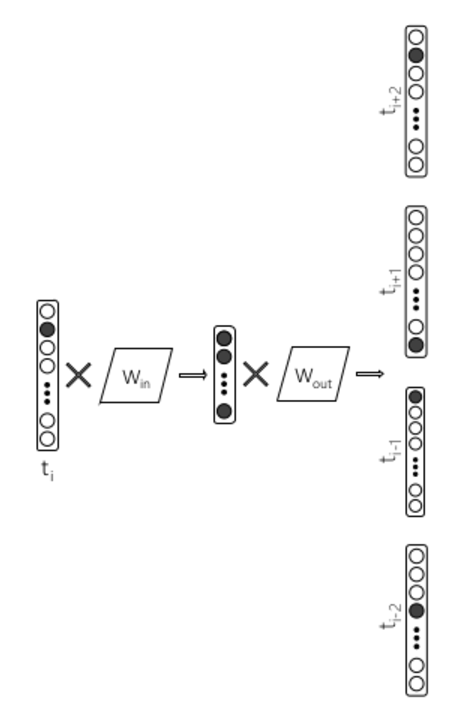
\includegraphics[scale=0.99]{Figures/skip_gram.eps}
		\caption{Diagram for Skip-Gram.}
		\label{chap:word_embeddingss:fig:skipgram_diagram}
	\end{center}
\end{figure}

Finally, the above neural models, either CBOW or skip-grams, since they are approximating the continuous distribution probability function of words over the the Vocabulary $V$ they also satify the following constraint:

\begin{equation} \label{chap:word_embeddings:eq:nnet_condtraint}
	\sum_{i=1}^{|V|}{p(t_{i}|t_{i-k}, ... ,t_{i+k})} = 1
\end{equation}

Note that in both CBOW and skip-gram models the two weight matrices $W_{in}$ and $W_{out}$ can be used to provide the word embeddings\footnote{An implementation of these methods is provided in https://github.com/tmikolov/word2vec}. Usually $W_{in}$ plays this role and $W_{out}$ is discarded.

\textcolor{red}{THIS IS NOT CLEAR: A very important difference between the CBOW and skip-grams is the NNet architecture usually their implementation is based. Particularly, there are some internal detail occurring because of the objective of the task. \parencite{boden2002guide}}

To summarize, the above models are very effective \textit{Language Modeling} approaches having the ability to quantify simultaneously syntanctic and semantic information of words. They provide a \textit{distributed representation} for words (i.e., each word is represented with a dense vector which is a point in a space of relatively low dimensionality). The sequence of words in texts is now considered and can also be applied in cases input texts are composed of seguences of characters or POS tags.

Finally, the training of the CBOW and the skip-gram models can be expensive despite the fact of limiting the number of hidden layers. However, there are several engineering solution that are accelerating the training time, such as \textit{Huffman binary Tree encoding} of words and \textit{hierarchical soft-max}. The latter is a solution that enables us to use multi-processing power and update the weight parameters concurrently. The parallel asynchronous updating of the parameter matrices is not conforming to the mathematical constraints however in practice the negative effect is minor. Huffman binary tree is a method for compressing the encoding of terms where the ones with the higher frequency are accessed faster. In addition to this, \textit{negative sampling}, \textit{sub-sampling}, or \textit{ramdom sampling} are also used where in the range of $k$ window for surrounding words only a few are selected during training with minor effect in  performance and significant acceleration in training \parentcite{mikolov2013efficient,mitra2018introduction}. 

\subsection{Document Embeddings} \label{chap:word_embeddings:sec:PVBOW} 
 
There are several approaches to tranform word embeddings to document embeddings \parencite{mitra2018introduction,mikolov2013distributed}. The most simple method produces a vector for a given document by averaging the word embeddings of the words in a document. It is also possible is to modify the network architecture and work on the sentence level. For example, word embeddings per sentence are averaged and the goal is to predict a sentence given its context sentences \parentcite{Kenter:2016}. Another idea, the \textit{Sent2Vec} method, is to compose sentence embeddingsby extending CBOW to include word vectors and word n-gram embeddings \footnote{An implementation of this method can be found in https://github.com/epfml/sent2vec}.

In this thesis, we use the \textit{Doc2Vec} approach introduced in \parentcite{le2014distributed}. that attempts to generalize the word embeddings methods to work with sequences of words. 


In this study, the Paragraph Vector Bag-of-Words (PV-BOW) model is used for the WGI task in the open-set framework evaluation. The PV-BOW is a DF modeling of the documents as an extension of the Skip-Grams modeling. The PV-BOW extends the idea of the \textit{Continues Distribution of the Words} over the Vocabulary and the Context defined by a Corpus of documents. A \textit{Continues Distribution of the Paragraphs (CDP} is defined where this method considers the concatenation of the paragraph vector with the word vectors to predict the next word in a text window. 
 
The CDP can be derived with two methods, one is based on CBOW and the other on Skip-Grams, which is used in this study. The CBOW extension is called Distributed Memory Paragraph Vector (PV-DM) because the Paragraph Vector is given as an input together with the word vectors, and it is considered as memory of the words distribution.
 
Another way is to ignore the context words in the input, and make a model for predicting words randomly sampled from the paragraph in the output. That is the Skip-gram model but instead of a words the whole paragraph vector is given as an input as shown in figure \ref{chap:word_embeddingss:fig:PVBOW_diagram}. In practice, at each iteration of stochastic gradient descent, text window of $k$ size is sampled. Then a random word sampled from the text window and form a classification task given the Paragraph Vector and  this is the PV-DBOW. This model requires to store less data, because only the softmax weights are stored as opposed to both softmax weights and word vectors in the PV-DM. 

\begin{figure}[t]
	\begin{center} 
      	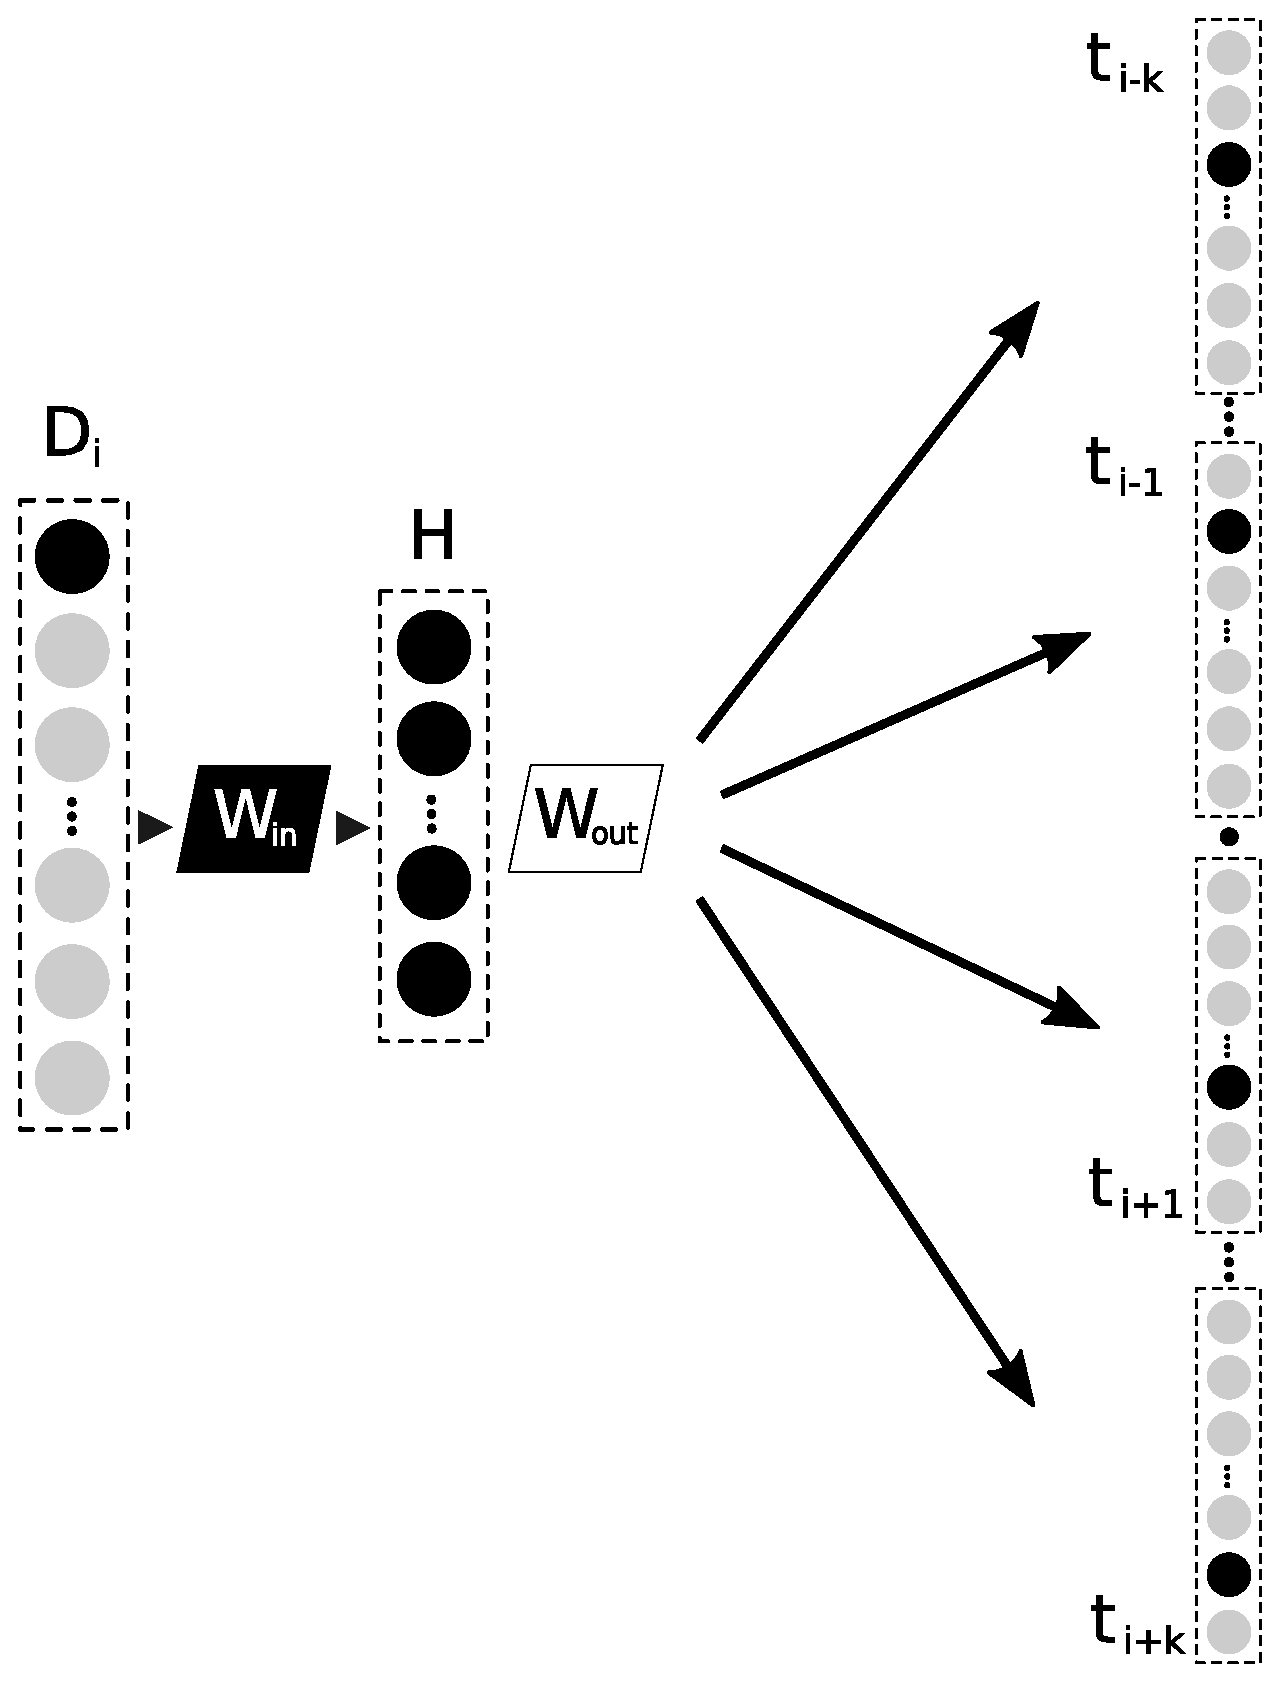
\includegraphics[scale=0.50]{Figures/pvbow.eps}
    		\caption{Diagram for PV-BOW}
		\label{chap:word_embeddingss:fig:PVBOW_diagram}
	\end{center}
\end{figure}


It should be noted that the Paragraph Vectors can be a text paragraph, a sentence, or the whole document. In this study, the whole web-pages is considered as shown in the first vector at the left in figure \ref{chap:word_embeddingss:fig:PVBOW_diagram}. There are several implementation for the PV-BOW modeling and a late evolution proposal for making the model more appreciate for IR problems. Including, \textit{Document frequency based Negative Sampling} and \textit{Document Length Regularization} \parencite{le2014distributed,posadas2017application}.

The PV-BOW objective log likelihood of Skip-gram models described in equation \ref{chap:word_embeddings:eq:skipgram_log_likelihood} is changing to the equation \ref{chap:word_embeddings:eq:pvbow_log_likelihood}  

\begin{equation} \label{chap:word_embeddings:eq:pvbow_log_likelihood}
	 \mathcal{L}_{SkipGram} = \frac{1}{|S|} \sum_{i=1}^{|S|}{ \sum_{-k \leq j \leq +k}{ \log {p(t_{i+j}|D_{i};\theta)}  } }
\end{equation}
\noindent
where $D_{i}$ is the Document Vector or Document ID, $S$ is the prediction windows over the training text and $k$ is the number of the words to be predicted surrounding the input word $\theta$ set of parameters to be optimized. Consequently,  the Softmax function is becoming as shown in equation \ref{chap:word_embeddings:eq:pvbow_softmax}.

\begin{equation} \label{chap:word_embeddings:eq:pvbow_softmax}
	p(t_{i+k}|t_{i}) = \frac{ e^{(W_{out}  \times  t_{i+j})^{T} (W_{in} \times  D_{i})}}{\sum^{|V|}_{i}{ e^{(W_{out}  \times  t_{k})^{T} (W_{in} \times  D_{i})}}} 
\end{equation}
Paragraph Vectors address some of the key weaknesses of bag-of-words (remember words can be any terms characters, words or POS) models. First, they capture the semantics of the terms. Therefore, words like “strong”  and "powerful" are closer together both and far from "Athens". Secondly, paragraph vectors take into consideration the word order, at least in sentence or paragraph level, in the same way that an Word n-Gram model would do in the size of n-Terms. As we will see experimentally the n-gram model also preserves a lot of information of the paragraph such as the word order. However, even if in some cases like in the experiments below, the n-grams perform equally to the PV-BOW DF models, the DF models can generalize better. They encoding more information with much denser and continuous dimemnsionality or at least the information they capture is not sparse and maybe "broken" in the small ranges of n-terms.

In practice a library for HTML reprocessing and and Vector Representation of the web-pages has been created for this work, named  \textit{Html2Vec}\footnote{\url{https://github.com/dpritsos/html2vec}}. There as special module for PV-BOW modeling has been build, where it is based on the the algorithm can be found at \textit{Gensim package} \footnote{\url{https://github.com/RaRe-Technologies/gensim}}. 


In this study a PVBOW Distributional Feature model for the whole corpus is trained. The corpus initially is split to a set of paragraphs, as required from PVBOW. To be more specific the paragraphs are sentences split from all the document of the whole corpus. Then several models PVBOW feature models are trained for a variety of parameters and vector dimensions, explained in the experiments section below. After the model has been fitted then one vector for each web-document was inferred from the PVBOW. The final document vectors derived from \tetxit{Distributional Feature Model} are given to the open-set learning model explained below. 


\section{Experimental Setup}\label{chap:word_embeddings:sec:experiments_setup}

%\subsection{Corpus}\label{chap:word_embeddings:sec:experiments_corpora}

The experiments of this chapter, are based on \textit{SANTINIS}, a benchmark corpus already used in previous work in WGI \parencite{mehler2010genres_on_web,pritsos2018open,santini2007automatic}. Briefly, this dataset comprises 1,400 English web-pages evenly distributed into seven genres (blog, eshop, FAQ, frontpage, listing, personal home page, search page) as well as 80 BBC web-pages evenly categorized into four additional genres (DIY mini-guide, editorial, features, short-bio). In addition, the dataset comprises a random selection of 1,000 English web-pages taken from the SPIRIT corpus \parencite{joho2004spirit}. The latter can be viewed as \textit{unstructured noise} since genre labels are missing. More details for SATNINIS corpus are discussed in section \ref{}. 


%\subsection{Open-set Models Parameters Setup}\label{chap:word_embeddings:sec:experiments_params}

To represent web-pages again the features are exclusively related to textual information, excluding any structural information, URLs, etc. The following representation schemes are examined: Character 4-grams (C4G), Word unigrams (W1G), and Word 3-grams (W3G). For each of these schemes, we use either Term-Frequency (TF) weights or DF features. The feature space for TF is defined by a vocabulary $V_{TF}$, which is extracted based on the most frequent terms of the training set --- we consider $V_{TF}=\{5k,10k,50k,100k\}$. The DF space is pre-defined in the PV-BOW model --- we consider $DF_{dim}=\{50,100,250,500,1000\}$.

In PV-BOW, the terms with very low-frequency in the training set are discarded. In this study, we examine $TF_{min}=\{3,10\}$ as cutoff frequency threshold. The text window size is selected from $W_{size}=\{3,8,20\}$. The remaining parameters of PV-BOW are set as follows: $\alpha=0.025$, $epochs=\{1, 3, 10\}$ and $decay=\{0.002, 0.02\}$. The PV-BOW creation process is also driven by an internal terms \textit{vocabulary} which is used for eliminating the terms with lower than a preferred frequency and then discards the terms from the text window for the PV-BOW (see section \ref{}).


Regarding the NNRD open-set classifier, there are two parameters, $lambda$ and DRT, and their considered values are: $\lambda =\{0.2, 0.5, 0.7\}$, $DRT\textit{=\{0.4, 0.6, 0.8, 0.9\}}$. All aforementioned parameters are adjusted based on grid-search using only the training part of the corpus.

For a proper comparison with prior art, the Random Feature Subset Ensemble (RFSE) and one-class SVM (OCSVM) \parencite{pritsos2013open,pritsos2018open} are used as baseline, the two open-set WGI approaches with good results presented in chapter \ref{chap:noise}. All parameters of these methods have been been adjusted as suggested in this section (for the same corpus).

The open-set evaluation framework is followed with \tetxit{unstructured noise} introduced in the preview section \ref{}. In particular, the open-set F1 score \parencite{mendesjunior2016} is calculated over the known classes (the noisy class is excluded). The reported evaluation results are obtained by performing 10-fold cross-validation and, in each fold, the full set of 1,000 \tetxit{noise pages} was included. 

This evaluation strategy is giving a more realistic evaluation. Since the noise size is greater than the size of any genre included in the given genres collection.

To compensate the unbalanced distribution of web pages over the genres because of the noise part, the macro-averaged precision and recall measures is used as explained in section \ref{} and also used in \parencite{mendesjunior2016}. Note again than this special modified method calculates precision and recall only for the known classes (available in the training phase) while the unknown samples (belonging to classes not available during training) affect false positives and false negatives. 

Finally, for selection parameter settings that obtain optimal evaluation performances the two scalar measures are used where their usage is reasoned in section \ref{}. Firstly, the \textit{Area Under the Precision-Recall Curve} (AUC) to the  standard \textit{11 Recall Levels} and particularly the Macro-AUC (MAUC). Secondly, the $F_{1}$ and specifically the Macro-F1 (MF1) score.


\section{Experimental Results}\label{chap:word_embeddings:sec:results}

\subsection{NNDR with DF or TF Features}\label{chap:word_embeddings:sec:NNDR_PVBOW_vs_BOW}

NNDR, analytically described in \ref{}, is an open-set formation of the NN algorithm. On the contrary to the previously discussed open-set algorithms such as the RFSE, it has the ability to explicitly parameterized for regulating the \textit{open space risk}. In this paragraph the NNRD performance is evaluated in the open-set with \textit{unstructured noise} conditions, using the SANTINIS corpus.

Additionally, since the noise-class is marked the algorithm is evaluated in both false-positive and the false-negative classifications of the marked-unknown-classes. The Macro-F1 and Macro-PRC are capturing the this error an penalizing the performance of the algorithm when this happens, as also explained in section\ref{} chapter 4.

Initially NNDR is evaluated in the BOW features with TF weighting schema vocabulary as shown in table \ref{chap:word_embeddings:tbl:NNDR_TF}. The overall performance is poor, however, better to the OCSVM's performance in table \ref{}, of section \ref{}. Constantly, to the experiments of chapter \ref{} the W3G is the \textit{terms type} where NNDR can have MAUC and MF1 over $0.66$. The algorithms parameters are also slightly affected for STP and SUP, while DRT in all cases is $0.8$. The $\lambda$ parameter has no effect, i.e. can be any value of the available set of these experiments. In should also be noted that the MF1 and the MAUC are both maximized for the same document representation, i.e. W3, the same vocabulary size, i.e. 10000, and the same algorithm parameters.

\begin{table}
\center
\begin{tabular}{cccclrrrrr}
\hline
STP & SUP & DRT & $\lambda$ & T.TYPE & DIMs & M\emph{P} & M\emph{R} & M\emph{AUC} & M\emph{F1} \\
\hline
0.7 & 0.3 & 0.8 & any & C4G & 5000 & 0.664 & 0.403 & 0.291 & 0.502 \\
0.7 & 0.5 & 0.8 & any & W1G & 5000 & 0.691 & 0.439 & 0.348 & 0.537 \\
0.5 & 0.5 & 0.8 & any & W3G & 10000 & 0.720 & 0.664 & 0.486 & 0.691 \\
\hline
\end{tabular}
\caption {Maximum performance of NNDR on TF Features of SANTINIS coprus. STP is the Spliting Training Percentage. SUP is the Splitting Unknown Percentage. DRT is the Distance Ration Threshold. $\lambda$ is the weigthing balance regulation parameters for the Normalized Accuracy. T.TYPE is the Terms Type. DIMs is the features model's dimensions. MP is the Macro Precision. MR is the Macro Recall. MAUC is the Area Under the Macro PR Curve. MF1 is the F1 score of the Macro Precision and Macro Recall.}
\label{chap:word_embeddings:tbl:NNDR_TF}
\end{table}



\begin{table}
\center
\begin{tabular}{cccclrrrrr}
\hline
STP & SUP & DRT & $\lambda$ & T.TYPE & DIMs & M\emph{P} & M\emph{R} & M\emph{AUC} & M\emph{F1} \\
\hline
any & any & 0.8 & any & C4G & 50 & \textbf{0.829} & 0.600 & 0.455 & 0.696 \\
any & any & 0.8 & any & W1G & 50 & 0.733 & 0.670 & 0.541 & 0.700 \\
any & any & 0.8 & any & W3G & 100 & 0.827 & 0.615 & 0.564 & \textbf{0.706} \\
\hline
\end{tabular}
\caption {Maximum performance of NNDR on Distributional Features of SANTINIS corpus. STP, SUP, DRT, $\lambda$, T.TYPE, DIMs are the same as in table \ref{tbl:NNDR_TF}. MTF is the Minimum Threshold Fequency of the Distributional models Vocabulary. WS is the Windows Size of the text sentence. $\alpha$ is the NNet parameter. EP is the epochs number of the NNet model. DEC is the decay parameter of the NNet model. MP is the Macro Precision. MR is the Macro Recall. MAUC is the Area Under the Macro PR Curve. MF1 is the F1 score of the Macro Precision and Macro Recall.}
\label{chap:word_embeddings:tbl:NNDR_PVBOW}
\end{table}

In the next evaluation step the NNDR has been tested using the PVBOW \textit{distributional features neural model }as described in section \ref{chap:word_embeddings:sec:PVBOW}. As shown in table \ref{chap:word_embeddings:tbl:NNDR_PVBOW} the performance of the algorithm has a significant improvement since the  MF1 from $0.691$ climbs to $0.706$ with the lowest performance at $0.696$ for C4G. It also should be noted that the is also maximized for the same parameters. 

The NNRD consistently returns is highest performance with the W3G for PVBOW model and for BOW TF vectors. The PVBOW seems to improve the $MP$ significantly by reaching the score of $0.829$ comparing to the initial maximum of $0.720$, with BOW. On the contrary to the BOW the maximum precision is returned with C4G while the maximum MF1 is returned for W3G. However, the precision score returned for W3G is very close to the one of C4G.

The PRC diagram is shown in figure  \ref{chap:word_embeddings:fig:NNDR_W3G} for having a better insight of the NNDR algorithm's improvement with the PVBOW neural language model compare to the BOW with TF weighting scheme. In particular, the W3G document representation is used for both diagrams of the NNDR because in both cases the $MACU$ and the MF1 are both maximized for either BOW or PVBOW.

\begin{figure}[H]

\begin{center}
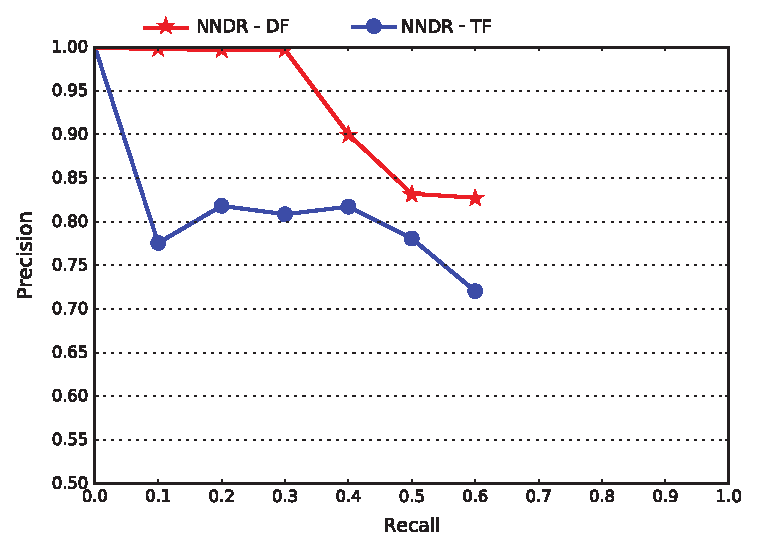
\includegraphics[scale=0.99]{Figures/NNDR_W3G.eps}
\caption{Precision-Recall Curves of NNDR on SANTINIS corpus. The curves are for W3G terms-type and for AUC optimization criterion. The 11-recall-levels are shown for each evaluation experiment. The lines are stopping before the 11th recall level due to the open-set framework, i.e. the remaining part after the last mark of each curve it the percentage of the corpus tha has been classified as Unknown from the algorithms.}
\label{chap:word_embeddings:fig:NNDR_W3G}
\end{center}

\end{figure}

The NNDR-DF is starting higher than NNDR-TF and it remains to $0.99$ precision for the $30\%$ of the corpus. Then it drops rgradualy and remains over $0.80$ up to $60\%$ of the corpus. The the rest of the corpus is classified as unknown. RFSE manages to recognize correctly part of the corpus up to $80\%$ with the precision to drop to $0.70$ and then to $0.65$. 

Considering the NNDR-TF is significantly lower in performance and for the first $10\%$ of the corpus is just above $0.75$. Given that the curves are calculated based on the ranked scores from the best performance to the lowest performance it seems that the algorithm significantly affected by the \textit{unstructured noise}. That is, the algorithm makes very confident decision for some part of the corpus confusing them with other classes. Its overall performance is over $0.7$ precision and also recognize the $60\%$ of the corpus, just like with the DF.

To conclude it seems that NNDR with distributional features is returning a significantly better performance than the BOW with TF weighting scheme. Although the $ΜR$ for PVBOW is slightly lower comparing the last row of both tables \ref{chap:word_embeddings:tbl:NNDR_TF} and \ref{chap:word_embeddings:tbl:NNDR_PVBOW}, the $MP$ is significantly higher. This is more important especially for the task o WGI in an open-set framework with noise, as explained in detail previously (see section \ref{}) in this thesis. 

In the next section the NNDR is compared to the RFSE and OCSVME open-set algorithms both described in \textit{chapter \ref{chap:openset}} and their evaluation experiments presented in \textit{chapter \ref{chap:noise}}.


\subsection{Comparison of Open-set WGI Methods}\label{chap:word_embeddings:sec:experiments_setup}

In this section the objective is to find out  how far the improvement of an open-set algorithm can go with the PVBOW neural language model compare to the RFSE and OCSVME as baselines. The baselines and NNDR are applied in the SANTINIS corpus. 

In the training phase, only the 11 known genre classes are use, while in test phase an additional class of the \textit{unstructured noise} is considered. Table\ref{chap:word_embeddings:tbl:NNDR_RFSE_OCSVME_final} shows the performance of tested methods when either TF or DF representation schemes, based on C4G, W1G, or W4G features, are used. 

\begin{table}[t]
\center
\caption {Performance of baselines and NNDR on the SANTINIS coprus. All evaluation scores are macro-averaged.}
\label{chap:word_embeddings:tbl:NNDR_RFSE_OCSVME_final}
\begin{tabular}{ccccccc}
\hline
Model & Features & Dim. & Precision & Recall & AUC & F1 \\
\hline
RFSE & TF-C4G & 50k & 0.739 & \textbf{0.780} & 0.652 & 0.759 \\
RFSE & TF-W1G & 50k & 0.776 & 0.758 & \textbf{0.657} & \textbf{0.767} \\
RFSE & TF-W3G & 50k & 0.797 & 0.722 & 0.615 & 0.758 \\
OCSVM & TF-C4G & 5k & 0.662 & 0.367 & 0.210 & 0.472\\
OCSVM & TF-W1G & 5k & 0.332 & 0.344 & 0.150 & 0.338\\
OCSVM & TF-W3G & 10k & 0.631 & 0.654 & 0.536 & 0.643\\
NNDR & TF-C4G & 5k & 0.664 & 0.403 & 0.291 & 0.502 \\
NNDR & TF-W1G & 5k & 0.691 & 0.439 & 0.348 & 0.537 \\
NNDR & TF-W3G & 10k & 0.720 & 0.664 & 0.486 & 0.691 \\
NNDR & DF-C4G & 50 & \textbf{0.829} & 0.600 & 0.455 & 0.696 \\
NNDR & DF-W1G & 50 & 0.733 & 0.670 & 0.541 & 0.700 \\
NNDR & DF-W3G & 100 & 0.827 & 0.615 & 0.564 & \textbf{0.706} \\
\hline
\end{tabular}
\end{table}

First, NNDR is compared with the baselines using TF features. In this case, NNDR outperforms OCSVM. On the other hand, RFSE performed better than NNDR for MF1 and MAUC. This is consistent for any kind of features (C4G, W1G, or W3G). There is notable difference in the dimensionality of representation used by the examined approaches though. RFSE relies upon a 50k-D manifold while NNDR and OCSVM are based on much lower dimensional spaces. 

The RFSE is the top performer while both OCSVME and NNDR are significantly low in respect of MAUC, MF1 and also MP.  Only, NNDR with TF scheme for W3G is competitive.

Next, NNDR with DF is compared with the same baselines and it self with BOW TF features. As shown in section \ref{chap:word_embeddings:sec:NNDR_PVBOW_vs_BOW} above there is a notable improvement for NNDR with DF features and now is comparable with RFSE baseline. 

However, still RFSE outperforms NNDR although the MF1 is comparable for all cases of features, i.e. W3G, W1G, C4G. On the other hand NNDR returns an notably higher performance from RFSE in respect of MP for C4G and W3G. It also to be noted that in all cases the selected value of parameter DRT is 0.8. This indicates that NNDR is a very robust algorithm.

The dimensionality of DF is much lower than TF and this seems to be crucial to improve the performance of NNDR. This is consistent for all three feature types (C4G, W1G, and W3G). It has to be noted that RFSE builds an ensemble by iteratively and \textit{randomly selecting} a subset of the available features. That way, it internally reduces the dimensionality for each constituent base classifier. RFSE is using about 1000 \textit{randomly selected features} from the 50,000 most frequent features. This observations together with the improvement of the NNDR performance with DF is a strong indication where the genre information is pervasive in several features of the texts and the magnitude of the features frequency is not enough. 

Finally, the proposed approach using NNDR and DF outperforms OCSVM but, as said above, it is outperformed by the strong baseline RFSE in both MAUC and MF1. However, when precision is concerned, NNDR is much better. A closer look at  the comparison of the two methods is provided in Fig. \ref{chap:word_embeddings:fig:NNDR_W3G_Best_RFSE_Baseline}, where MPRCs are depicted. 

The NNDR-DF model maintains very high precision scores for low levels of recall. Particularly, for W3G the difference between NNDR-DF and RFSE at that point is clearer. NNDR-TF is clearly worse than both NNDR-DF and RFSE. In addition, OCSVM is competitive in terms of precision only when W3G features are used but its performance drops abruptly in comparison to that of NNDR-DF. 

RFSE with W1G performs significantly better in terms of MP than NNDR (with DF). It also manages to recognize correctly larger part of the corpus, more than $70\%$ either for W3G or for W1G, compare to NNDR-DF that reaches $60\%$ in both left and right diagrams of figure \ref{chap:word_embeddings:fig:NNDR_W3G_Best_RFSE_Baseline}. Note that the point where the curves end indicates the percentage of corpus that is left unclassified because it is left unclassified as \tetxit{unknown class}.

\begin{figure}[t]
\begin{center}
    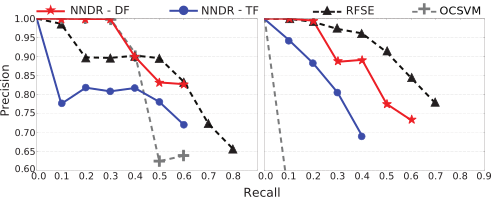
\includegraphics[scale=0.95]{Figures/NNDR_W3G-W1G_Best_RFSE-OCSVM-Baselines.eps}
	\caption{Precision curves in 11-standard recall levels of the examined open-set classifiers using either W3G features (left) or W1G features (right).}
	\label{chap:word_embeddings:fig:NNDR_W3G_Best_RFSE_Baseline}
	\end{center}
\end{figure}

%, i.e. the remaining part after the last mark of each curve it the percentage of the corpus tha has been classified as Unknown from the algorithms.

\section{Conclusions}\label{chap:word_embeddings:sec:conclusions}

In this chapter is presented an experimental study focused on WGI and the use of distributional features in combination with an open-set classifier that obtained promising results in other domains. Our experiments are based on a benchmark corpus already used in prior art and a strong baseline. Particularly it is evaluated the possible performance improvement of an open-set algorithm when distributional features are employed, using the SANTINIS corpus (i.e. a corpus with an unstructured noise).

It seems that distributional features provide a significant enhancement to the NNDR open-set method. The low-dimensionality of DF is crucial to boost the performance of NNDR. Yet, RFSE proves to be a hard-to-beat baseline at the expense of relying upon a much higher representation space (usually in the thousands of features). However, with respect to precision, the NNDR with PVBOW neural model input, is much more conservative and it prefers to leave web-pages unclassified rather than guessing an inaccurate genre label. Depending on the application of WGI, precision can be considered much more important than recall and this is where the proposed approach shines, i.e an open-set algorithm combined with \tetxit{neural language model}.

The open-set algorithm NNDR have been evaluated with distributional features which have been described in detail in chapter \ref{chap:openset}. A \textDistance Ration threshold is calculated while the training procedure for maximizing the \textit{Normalized Accuracy} of the known and the unknown classes.

The evaluation methodology previews shown to be proper for evaluation open-set scenarios. The natural focus in an open-set evaluation framework is the macro-precision, because always there is a part of the corpus will be classified as unknown. Either in the case of structured and unstructured or it is considered as outage while training.

Further research could focus on more appropriate distance measures within NNDR specially with recent data-driven features obtained with powerful NLP convolutional and recurrent deep networks. Moreover, alternative types of distributional features could be used (e.g., topic modeling). Finally, a combination of NNDR with RFSE models could be studied as they seem to exploit complementary views of the same problem.


\include{Chapters/Clustering}


%----------------------------------------------------------------------------------------
%	BIBLIOGRAPHY
%----------------------------------------------------------------------------------------
\printbibliography[heading=bibintoc]


\end{document}
